% Build from reports/: latexmk -pdf -interaction=nonstopmode final_thesis.tex
\documentclass[12pt,a4paper]{report}

\usepackage[vmargin=2.5cm,hmargin=3cm]{geometry}
\usepackage[T1]{fontenc}
\usepackage[utf8]{inputenc}
\usepackage[english]{babel}
\usepackage{microtype}
\usepackage{amsmath,amssymb}
\usepackage{txfonts}
\usepackage{booktabs}
\usepackage{tabularx}
\usepackage{multirow}
\usepackage[table]{xcolor}
\usepackage{graphicx}
\usepackage{tikz}
\usetikzlibrary{arrows.meta,positioning,calc,fit,backgrounds,shapes.geometric}
\usepackage{pgfplots}
\pgfplotsset{compat=1.18}
\usepackage{float}
\usepackage{caption}
\usepackage{subcaption}
\usepackage{fancyhdr}
\usepackage{titlesec}
\usepackage{titletoc}
\usepackage{enumitem}
\usepackage{needspace}
\usepackage{longtable}
\usepackage{listings}
\usepackage{seqsplit}
\usepackage[numbers,sort&compress]{natbib}
\usepackage{hyperref}

\definecolor{azulUC3M}{RGB}{0,0,102}
\definecolor{safety}{HTML}{A8322D}
\definecolor{block}{HTML}{255F85}
\definecolor{good}{HTML}{2D7D46}
\definecolor{warn}{HTML}{D88324}
\definecolor{line}{HTML}{D7DED8}
\definecolor{softblue}{HTML}{E8F0F8}
\definecolor{softgreen}{HTML}{E8F3EB}
\definecolor{softorange}{HTML}{FAEEDD}
\definecolor{softpurple}{HTML}{EEE8F4}
\definecolor{pidP}{HTML}{2F6DB0}
\definecolor{pidI}{HTML}{D88324}
\definecolor{pidD}{HTML}{7A4FA3}
\definecolor{pidFuse}{HTML}{2D7D46}

\newcommand{\MasterDegree}{Master in Connected Industry 4.0}
\newcommand{\ThesisAuthor}{Samer Awad}
\newcommand{\ThesisTutor}{Alberto Jiménez Hormeño}
\newcommand{\AcademicYear}{2025--2026}
\newcommand{\SubmissionPlaceDate}{Madrid, July 2026}
\newcommand{\ThesisTitle}{Learning Binary Traversability from Monocular RGB for Off-Road Navigation}
\newcommand{\FSR}{\mathrm{FSR}}
\newcommand{\FBR}{\mathrm{FBR}}

\hypersetup{
  colorlinks=true,
  linkcolor=black,
  citecolor=black,
  urlcolor=blue,
  pdftitle={\ThesisTitle},
  pdfauthor={\ThesisAuthor},
  pdfsubject={Master Thesis, Universidad Carlos III de Madrid},
  pdfkeywords={traversability, semantic segmentation, PIDNet, ROD, CaT, asymmetric error metrics, real-time inference, reproducibility}
}

\pagestyle{fancy}
\fancyhf{}
\renewcommand{\headrulewidth}{0pt}
\rfoot{\thepage}
\fancypagestyle{plain}{
  \fancyhf{}
  \renewcommand{\headrulewidth}{0pt}
  \rfoot{\thepage}
}

\titleformat{\chapter}[block]{\large\bfseries\filcenter}{\thechapter.}{5pt}{}
\titlespacing{\chapter}{0pt}{0pt}{*3}
\titleformat{\section}{\bfseries}{\thesection.}{5pt}{}
\titleformat{\subsection}{\normalsize\bfseries}{\thesubsection.}{5pt}{}
\titlecontents{chapter}[0pt]{}
  {\contentsmargin{0pt}\thecontentslabel.\enspace}
  {\contentsmargin{0pt}}
  {\titlerule*[.7pc]{.}\contentspage}
\titlecontents{section}[5pt]{}
  {\contentsmargin{0pt}\thecontentslabel.\enspace}
  {\contentsmargin{0pt}}
  {\titlerule*[.7pc]{.}\contentspage}

\setcounter{tocdepth}{2}
\setcounter{secnumdepth}{2}
\setlength{\parskip}{6pt}
\setlength{\emergencystretch}{1.5em}
\renewcommand{\baselinestretch}{1.15}
\setlist{itemsep=2pt,topsep=3pt}

\captionsetup[table]{
  name=TABLE,
  justification=centering,
  labelsep=period,
  labelfont=small,
  font=small
}
\captionsetup[figure]{
  name=Fig.,
  format=hang,
  singlelinecheck=off,
  labelsep=period,
  labelfont=small,
  font=small
}

\lstset{
  basicstyle=\ttfamily\footnotesize,
  breaklines=true,
  columns=fullflexible,
  frame=single,
  rulecolor=\color{line},
  showstringspaces=false
}

\begin{document}
\hypersetup{pageanchor=false}
\pagenumbering{roman}

\begin{titlepage}
  \begin{sffamily}
  \color{azulUC3M}
  \begin{center}
    \makebox[\textwidth][c]{%
      
\includegraphics[width=16cm]{figures/uc3m_logo.png}%
    }

    \vspace{1cm}
    {\Large
      \MasterDegree\\
      \AcademicYear\\[1cm]
      \textsl{Master Thesis}
    }

    \bigskip
    \begin{minipage}{0.96\textwidth}
      \centering
      {\Huge ``\ThesisTitle''\par}
    \end{minipage}

    \vspace{0.5cm}
    \rule{10.5cm}{0.1mm}\\[0.9cm]
    {\LARGE \ThesisAuthor}\\[1cm]
    {\Large
      Tutor\\
      \ThesisTutor\\[0.18cm]
      \SubmissionPlaceDate
    }
  \end{center}

  \vfill
  \end{sffamily}
\end{titlepage}

% Blank courtesy verso required by the UC3M library template.
\setcounter{page}{2}
\clearpage
\thispagestyle{empty}
\null
\clearpage

% Optional author-specific front matter, as seen in the reference thesis:
% \clearpage
% \chapter*{Acknowledgements}
% \addcontentsline{toc}{chapter}{Acknowledgements}
% Replace this comment with the author's own acknowledgement text.

\hypersetup{pageanchor=true}

\chapter*{Abstract}
\addcontentsline{toc}{chapter}{Abstract}

Traversability perception estimates which parts of a visible scene a specific
vehicle can negotiate. This thesis formulates that task as binary semantic
segmentation from one RGB image using the vehicle-capability annotations of
the CaT dataset. The released labels are converted into two documented
policies. The principal blue+green policy treats the sedan and pickup regions
as traversable while retaining background and off-road-only terrain as
blocked. A deterministic split of the official training partition provides
validation data, and all 544 released test images are reserved for evaluation.

PIDNet-S is first used to establish the data and evaluation pipeline and to
test loss design, augmentation, class weighting, resolution, and decision
threshold. Its separately retained reference checkpoint achieves 0.8939 mean
Intersection over Union (mIoU), a 4.32\% False-Safe Rate (FSR), and a 7.04\%
False-Block Rate (FBR). A separate CPU evaluation reproduces all four confusion
counts over 133,693,440 pixel decisions. The model processes 21.16 frames per
second (FPS) on an AMD Ryzen~5~5500 when the model forward pass and prediction
are timed, and 106.43 FPS after TensorRT conversion on an NVIDIA RTX~5060 when
preprocessing, inference, and mask return are timed.

The architecture study compares PIDNet-S with frozen-encoder ROD and seven
other compact systems. An initial 15-epoch matrix supplies a matched
fixed-budget comparison under blue-only and blue+green policies. Because the
validation histories were still improving, a three-seed blue+green follow-up
uses a 300-epoch ceiling, 60-epoch cosine decay, and validation-based early
stopping. All nine models achieve higher mean test mIoU than under the fixed
15-epoch budget. FPN/EfficientNet-B0 obtains the largest mean
test mIoU ($0.9423\pm0.0005$), followed by U-Net/EfficientNet-B0
($0.9409\pm0.0004$); validation selects checkpoints between epochs 50 and 141.
Runtime rankings differ: PIDNet-S leads the H100 measurements, while
DDRNet-23-Slim leads the compiled CPU comparison.

Examples selected at several error percentiles, together with cases ranked by
false-safe, false-block, and boundary error, connect the aggregate scores to
the spatial form of the mistakes. Unlabelled ALICE sequences illustrate
cross-domain output behaviour but provide no accuracy measurement. These
findings support real-time pixel-level perception, but they do not certify that
vehicle motion is safe: a single RGB image hides relevant physical properties,
capability boundaries may be uncertain, and neither planning nor vehicle-level
behaviour is evaluated.

\noindent\textbf{Keywords:} traversability estimation; semantic segmentation;
PIDNet; ROD; CaT dataset; safety-oriented evaluation; real-time inference;
TensorRT; reproducibility.

\clearpage
\chapter*{Resumen}
\addcontentsline{toc}{chapter}{Resumen}

La percepción de transitabilidad estima qué regiones visibles puede recorrer
un vehículo determinado. Esta tesis formula la tarea como segmentación
semántica binaria de una imagen RGB mediante las anotaciones de capacidad
vehicular de CaT. Las etiquetas se convierten en dos políticas explícitas. La
política principal azul+verde considera transitables las regiones anotadas como
aptas para turismos o camionetas, y mantiene como no transitables el fondo y
las regiones reservadas a vehículos todoterreno. Una división determinista de
la partición oficial de entrenamiento proporciona los datos de validación,
mientras que las 544 imágenes oficiales de prueba se reservan para la
evaluación.

PIDNet-S establece el flujo experimental y permite estudiar la pérdida, el
aumento de datos, la ponderación, la resolución y el umbral. El modelo
seleccionado alcanza un mIoU de 0,8939, una
tasa de falso seguro del 4,32\% y una tasa de falso bloqueo del 7,04\%. Una
evaluación independiente en CPU reproduce los cuatro recuentos de la matriz de
confusión sobre 133.693.440 decisiones de píxel. El modelo procesa 21,16
imágenes por segundo en un AMD Ryzen~5~5500 cuando se cronometran el pase hacia
delante y la predicción, y 106,43 imágenes por segundo tras la conversión a
TensorRT en una NVIDIA RTX~5060 cuando se cronometran el preprocesamiento, la
inferencia y la devolución de la máscara.

El estudio compara PIDNet-S con ROD, cuyo codificador permanece congelado, y
otros siete sistemas compactos. Una primera matriz de 15 épocas proporciona
un presupuesto idéntico para las políticas azul y azul+verde. Como la
validación seguía mejorando, un segundo experimento azul+verde con tres
semillas utiliza un máximo de 300 épocas, decaimiento cosenoidal durante 60 épocas
y parada temprana. Los nueve modelos obtienen un mIoU medio de prueba superior
al alcanzado con el presupuesto fijo de 15 épocas. FPN/EfficientNet-B0 obtiene
el mayor mIoU medio ($0{,}9423\pm0{,}0005$), seguido de U-Net/EfficientNet-B0
($0{,}9409\pm0{,}0004$). Los puntos de control seleccionados mediante
validación corresponden a épocas comprendidas entre 50 y 141. En cuanto a la
velocidad, PIDNet-S alcanza el mayor rendimiento en la H100 y
DDRNet-23-Slim encabeza la comparación compilada en CPU.

Los ejemplos seleccionados por percentiles de error y los casos ordenados por
falso seguro, falso bloqueo y error de frontera relacionan las métricas
agregadas con la forma espacial de los errores. Las secuencias de ALICE, al no
estar anotadas, solo ilustran el comportamiento del modelo fuera del dominio de
CaT. Los resultados muestran una percepción por píxel útil en tiempo real, pero
no certifican que el movimiento del vehículo sea seguro.

\noindent\textbf{Palabras clave:} transitabilidad; segmentación semántica;
PIDNet; ROD; CaT; métricas de error asimétricas; inferencia en tiempo real;
reproducibilidad.

\clearpage
\chapter*{Notation and Acronyms}
\addcontentsline{toc}{chapter}{Notation and Acronyms}
\begin{longtable}{@{}p{0.18\textwidth}p{0.76\textwidth}@{}}
\toprule
\textbf{Term} & \textbf{Meaning in this thesis} \\
\midrule
ALICE & Unlabelled external mobile-robot sequences used only for qualitative transfer. \\
CaT & CAVS Traversability dataset. \\
CNN & Convolutional neural network. \\
CPU / GPU & Central processing unit / graphics processing unit. \\
FBR & False-Block Rate: fraction of truly traversable pixels predicted blocked. \\
FPN & Feature Pyramid Network. \\
FP, FN, TP, TN & False positive, false negative, true positive, and true negative, with traversable defined as positive. \\
FPS & Frames per second, always tied to a declared timing scope. \\
FSR & False-Safe Rate: fraction of truly untraversable pixels predicted traversable. \\
H100 MIG & The NVIDIA H100 NVL 3g.47GB multi-instance GPU partition used for common server timing. \\
IoU / mIoU & Intersection over Union for one class / unweighted mean across the two binary classes. \\
PIDNet-S & Small PIDNet variant used as the main lightweight baseline. \\
ROD & RGB-Only Fast and Efficient Off-road Freespace Detection model adapted to CaT. \\
RGB & Red, green, and blue image channels. \\
SMP & \texttt{segmentation-models-pytorch}, used for FPN, U-Net, and SegFormer implementations. \\
TensorRT & NVIDIA inference compiler/runtime used for the optimised RTX~5060 deployment measurements. \\
ViT-S & Small Vision Transformer encoder variant. \\
\bottomrule
\end{longtable}

\clearpage
\tableofcontents
\clearpage
\phantomsection
\addcontentsline{toc}{chapter}{List of Figures}
\listoffigures
\clearpage
\phantomsection
\addcontentsline{toc}{chapter}{List of Tables}
\listoftables
\clearpage
\pagenumbering{arabic}

% ============================================================
\chapter{Introduction}
\label{ch:introduction}
% ============================================================

\section{Motivation}

Autonomous driving on a paved road is supported by a set of regularities:
lanes have conventional widths, curbs provide visible boundaries, signs encode
rules, and the road surface is designed for ordinary vehicles. An off-road
vehicle encounters none of these guarantees. A pale strip in an image may be
compacted gravel, loose soil, shallow water, or a patch of dry vegetation.
The border between a track and its surroundings can be gradual, interrupted,
or hidden by shadow. Even if the surface category were recognised perfectly,
the answer to ``can the vehicle cross it?'' would still depend on clearance,
traction, wheelbase, mass, slope, and current conditions.

Traversability is therefore an \emph{affordance}: it describes what a particular
platform can do in a scene. The same region may be accessible to a pickup,
outside a sedan's capability, and trivial for a dedicated off-road vehicle. This
vehicle dependence makes traversability more operational than ordinary
terrain classification. It also creates a demanding perception problem,
because some of the relevant physical properties are not directly observable
from one RGB frame~\cite{islam2022review,sevastopoulos2022survey}.

The practical output considered in this thesis is a dense binary mask. Every
image pixel is labelled either traversable or untraversable for a declared
vehicle-capability policy. A mask is convenient for downstream processing: a
planner can intersect it with a projected footprint, inflate blocked regions,
or combine it with geometric and temporal estimates. Dense prediction also
exposes the spatial structure of errors. A connected false-safe region directly
in front of the vehicle has a different operational meaning from a handful of
isolated pixels at the top of the image, even if both contribute the same
number of errors to a global score.

Two competing engineering requirements motivate the study. First, the mask
must be accurate enough to represent narrow corridors and irregular
boundaries. Second, it must be produced fast enough for an onboard navigation
loop. A large pretrained transformer may supply strong visual features, while
a purpose-built real-time network may offer far lower latency. The thesis
therefore studies accuracy, asymmetric error rates, reproducibility, and
hardware speed together rather than treating any one of them as a complete
measure of success.

\Needspace{0.42\textheight}
\section{Problem Definition and Research Questions}

For an RGB image
\begin{equation}
  x\in\mathbb{R}^{H\times W\times3},
\end{equation}
where $x$ is the input tensor, $H$ and $W$ are its height and width in pixels,
the final dimension contains the red, green, and blue channels, and
$\mathbb{R}$ denotes real-valued samples. The system estimates a traversable
probability for each pixel and produces
\begin{equation}
  \hat y_{ij} =
  \mathbb{1}\!\left[p(y_{ij}=1\mid x)\geq \tau\right],
  \qquad
  \hat y\in\{0,1\}^{H\times W},
  \label{eq:intro_decision}
\end{equation}
Here, $i\in\{1,\ldots,H\}$ and $j\in\{1,\ldots,W\}$ index the pixel row and
column; $y_{ij}$ is its target class; $p(y_{ij}=1\mid x)$ is the model's
conditional probability of the traversable class; $\mathbb{1}[\cdot]$ is one
when its condition is true and zero otherwise; and $\hat y_{ij}$ is the
resulting binary prediction. Class 1 is traversable, class 0 is
untraversable, and $\tau$ is the fixed decision threshold. The complete
predicted mask $\hat y$ therefore has the same $H\times W$ spatial dimensions
as the image. The main PIDNet-S development uses $\tau=0.50$ and the
CaT blue+green policy: sedan- and pickup-traversable pixels are positive,
while background and off-road-vehicle-only pixels are negative. The
architecture experiment also evaluates the more conservative blue-only policy.

This definition makes the two error directions explicit. A false positive
opens a pixel that the annotation declares blocked; it is called a
\emph{false safe}. A false negative rejects a pixel that the annotation
declares traversable; it is called a \emph{false block}. The first can expose a
planner to terrain outside the selected capability envelope. The second can
remove a feasible route or cause unnecessary stopping. The costs are
asymmetric, but they are not completely described by their pixel counts:
location, connectedness, vehicle speed, and the planner all affect the
consequence.

The investigation is organised around four research questions:
\begin{enumerate}
  \item Can PIDNet-S provide a reproducible, real-time baseline for the CaT
  binary task using only the official training partition?
  \item Which of the tested training and postprocessing choices materially
  change its accuracy, false-safe behaviour, and false-block behaviour?
  \item How does frozen-encoder transfer in ROD compare with PIDNet-S under
  matched seeds, and where do both systems lie among other compact
  segmentation architectures?
  \item How do the accuracy rankings change when inference latency, target
  hardware, execution runtime, and timing scope are included?
\end{enumerate}

\section{Objectives}

The investigation has four methodological objectives:
\begin{enumerate}
  \item define a reproducible binary task from the released CaT files,
  including explicit vehicle policies and a development split that does not
  draw from the official test partition;
  \item determine how a compact PIDNet-S implementation responds to changes in
  training objective, augmentation, class weighting, resolution, and
  threshold, while preserving the complete record of the selected model;
  \item compare that model with frozen-encoder ROD and a representative group
  of compact convolutional and transformer systems under repeatable training
  conditions;
  \item relate overlap quality and asymmetric errors to observed latency on
  CPU, H100, and TensorRT execution rather than using parameter count as a
  proxy for deployability.
\end{enumerate}

\section{Research Design}

The experiments were organised in two linked stages. The first stage treated
PIDNet-S as an engineering reference. Building that model required decisions
about file pairing, target conversion, augmentation, loss terms, validation,
error reporting, and export. Exploratory runs exposed interactions between
several of those choices; a subsequent single-factor study separated them.
The selected checkpoint was retained unchanged so that its numerical,
qualitative, and runtime measurements all refer to the same parameters.

The second stage asked whether the conclusion depended on that initial
architecture. ROD introduced a pretrained transformer whose encoder remained
fixed during CaT training. A matched PIDNet--ROD experiment measured the
difference over three seeds, after which seven additional systems supplied
context for the pairwise result. The first matrix used a common 15-epoch
budget under both label policies. Its validation histories showed that this
was useful as a fixed-budget comparison but too early to represent the models'
attainable performance. A convergence-aware follow-up therefore repeated the
principal blue+green matrix with a longer ceiling and validation-based stopping.
This order separates three questions that are often conflated: how one model
was engineered into a reproducible system, how complete model recipes compare
under equal training exposure, and how that ranking changes when each run is
allowed to progress beyond the early fixed budget.

\begin{figure}[htbp]
\centering
\resizebox{\textwidth}{!}{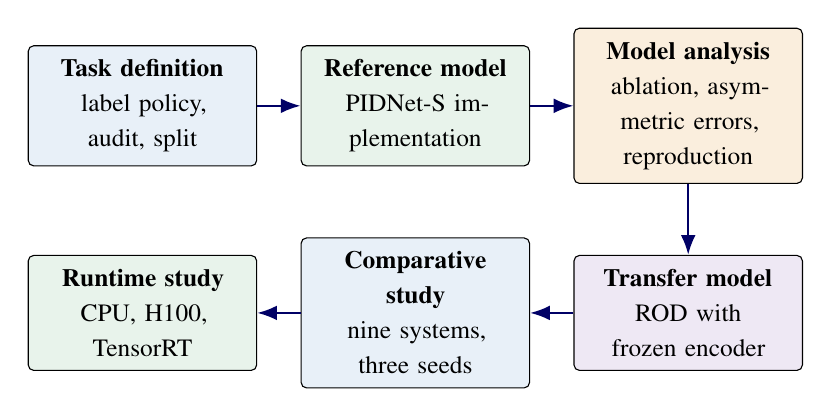
\begin{tikzpicture}[
  node distance=0.55cm,
  stage/.style={draw,rounded corners=2pt,minimum height=1.15cm,text width=2.55cm,
    align=center,font=\small,inner sep=5pt},
  arrow/.style={-{Latex[length=2.5mm]},thick,draw=azulUC3M}
]
\node[stage,fill=softblue] (task) {\textbf{Task definition}\\label policy, audit, split};
\node[stage,fill=softgreen,right=of task] (pid) {\textbf{Reference model}\\PIDNet-S implementation};
\node[stage,fill=softorange,right=of pid] (safe) {\textbf{Model analysis}\\ablation, asymmetric errors, reproduction};
\node[stage,fill=softpurple,below=0.9cm of safe] (rod) {\textbf{Transfer model}\\ROD with frozen encoder};
\node[stage,fill=softblue,left=of rod] (wide) {\textbf{Comparative study}\\nine systems, three seeds};
\node[stage,fill=softgreen,left=of wide] (deploy) {\textbf{Runtime study}\\CPU, H100, TensorRT};
\draw[arrow] (task) -- (pid);
\draw[arrow] (pid) -- (safe);
\draw[arrow] (safe) -- (rod);
\draw[arrow] (rod) -- (wide);
\draw[arrow] (wide) -- (deploy);
\end{tikzpicture}
}
\caption[Experimental structure.]{Experimental structure. A fixed task
definition connects model development, repeatability analysis, architectural
comparison, and hardware measurement.}
\label{fig:research_progression}
\end{figure}

Figure~\ref{fig:research_progression} summarises this progression from a fixed
task definition to model development, comparison, and hardware evaluation.

The validation-selected PIDNet-S checkpoint and the three-seed comparison are
therefore reported separately. The former is an artifact-level result backed
by exact reproduction and deployment measurements. The latter estimates
between-run variation under a common recipe. Combining them into one average
would erase the experimental conditions that give each number its meaning.

\section{Contributions}

The resulting contributions are:
\begin{itemize}
  \item an audited conversion of 1,812 underlying CaT samples to binary
  traversability, with an unchanged 544-image official test partition excluded
  from training and validation splitting and a
  deterministic 1,002/266 train--validation split;
  \item a detailed implementation of PIDNet-S for two-class prediction,
  including its tensor shapes, objective, optimisation, decision threshold,
  and controlled ablation history;
  \item a 7,623,522-parameter PIDNet-S checkpoint with 0.893941 mIoU,
  4.3176\% FSR, 7.0369\% FBR, and an exactly reproduced confusion matrix
  covering 133,693,440 pixel decisions;
  \item percentile-based and failure-ranked qualitative evidence that connects
  the aggregate asymmetric error rates to visible spatial behaviour;
  \item a CaT implementation of ROD with a frozen EfficientSAM ViT-S encoder
  and an explicit reconstruction of the published training regime;
  \item a nine-system, three-seed comparison under both blue-only and
  blue+green policies, including a $2\times2$ FPN/U-Net by
  MobileNetV2/EfficientNet-B0 design;
  \item a convergence-aware three-seed follow-up for the principal blue+green
  policy, with 27 validation-selected checkpoints, complete test records, and
  checkpoint identities;
  \item hardware measurements that distinguish forward-only CPU and H100
  timing from a larger TensorRT preprocessing-to-returned-mask scope.
\end{itemize}

\section{Scope and Responsible Interpretation}

This thesis studies monocular RGB segmentation. It does not estimate depth,
slope, soil strength, wheel slip, water depth, or a dynamically feasible
trajectory. The term \emph{safe} is retained in the metric name ``False Safe
Rate'' because it describes the binary label convention, not because the
network output certifies safe vehicle motion. A deployed system would require
sensor fusion, uncertainty handling, planner constraints, and vehicle-level
validation.

The quantitative claims are restricted to CaT, the two stated binary policies,
the declared seeds, and the saved protocols. Frames from the external ALICE
mobile-robot sequences are used only for qualitative transfer because no
ground truth is available. Hardware rates are not interchangeable: changing
the processor, runtime, numerical precision, batch size, input resolution, or
the start and end of the timer changes the meaning of FPS.

The CaT labels are treated as the reference for scoring, but not as a perfect
measurement of physical reality. Some boundaries are difficult to justify
from RGB appearance alone and may depend on physical information or subjective
vehicle-capability judgement unavailable to the model and thesis author.
Specific examples and the limits of that observation are discussed in
Chapters~\ref{ch:cat_pipeline},~\ref{ch:results}, and~\ref{ch:discussion}.

\section{Thesis Organisation}

Chapter~\ref{ch:background} introduces traversability perception, relevant
datasets, segmentation architectures, and CaT literature.
Chapter~\ref{ch:cat_pipeline} explains the CaT release, binary label policies,
split, preprocessing, and common software pipeline.
Chapter~\ref{ch:pidnet} presents the PIDNet-S implementation, exploratory
experiments, and controlled ablation.
Chapter~\ref{ch:rod_extension} introduces ROD and defines the comparative
architecture study.
Chapter~\ref{ch:protocols} defines training, evaluation, qualitative,
reproducibility, and timing protocols.
Chapters~\ref{ch:results} and~\ref{ch:hardware} report accuracy,
safety-oriented error metrics,
qualitative behaviour, and hardware speed.
Chapter~\ref{ch:discussion} analyses the trade-offs, limitations, and future
work; Chapter~\ref{ch:conclusions} summarises the evidence in relation to the
research questions.
Detailed configurations and reproduction commands are provided in the
appendices.

% ============================================================
\chapter{Background and Related Work}
\label{ch:background}
% ============================================================

\section{Traversability as Perception of an Affordance}

Traversability estimation asks whether a mobile platform can move through a
region of the environment. This differs from semantic terrain recognition.
The class ``grass'', for example, does not determine whether the surface is
load-bearing, whether vegetation hides a ditch, or whether the slope exceeds
the vehicle's limits. Conversely, several semantic materials can form one
continuous traversable corridor. Surveys therefore describe traversability as
a combination of geometric, appearance-based, semantic, and
vehicle-interaction evidence~\cite{islam2022review,sevastopoulos2022survey}.

Geometric approaches use LiDAR, stereo, or structured depth to estimate slope,
roughness, steps, and obstacle height. They offer direct evidence for some
physical constraints, but flat vegetation, water, deformable soil, and sparse
returns remain difficult. Appearance-based systems use colour, texture, shape,
and learned context from RGB images. They are inexpensive and information-rich
but cannot reliably infer every physical property. A multimodal system can
combine both strengths at the cost of calibration, synchronisation, sensor
weight, and computation.

Another distinction concerns the source of supervision. Human annotation can
describe regions that appear suitable for a vehicle. Self-supervised systems
can learn from wheel slip, suspension response, vehicle tracks, or a geometric
teacher. Interaction-derived labels are platform-specific, but they cover only
terrain the robot visits and inherit the assumptions of the teacher signal.
The present study uses a human-annotated dataset because it enables every model
to receive exactly the same dense target. This makes architectural comparison
possible, while leaving the physical validity of the labels as an explicit
limitation.

\section{Off-Road Perception Datasets}

Off-road datasets vary in their task, sensors, geography, and label semantics.
RUGD supplies dense outdoor semantic labels in unstructured scenes
~\cite{wigness2019rugd}. RELLIS-3D combines RGB and LiDAR at an off-road
proving ground~\cite{jiang2021rellis}. TartanDrive emphasises multimodal
sequences and vehicle dynamics~\cite{triest2022tartandrive}. ORFD targets
off-road freespace detection with RGB and LiDAR-derived information
~\cite{min2022orfd}. WildScenes provides repeated natural-environment
traversals with calibrated image and LiDAR data, enabling 2D, 3D, and
domain-adaptation studies~\cite{vidanapathirana2025wildscenes}.

Table~\ref{tab:background_datasets} summarises the sensing modalities and label
scope of these datasets relative to the monocular binary task used here.

\begin{table}[H]
\centering
\caption{Representative off-road datasets and their relation to this work.}
\label{tab:background_datasets}
\small
\begin{tabularx}{\textwidth}{@{}lrrlX@{}}
\toprule
\textbf{Dataset} & \textbf{Year} & \textbf{Images} & \textbf{Primary data} & \textbf{Main label or research focus} \\
\midrule
RUGD~\cite{wigness2019rugd} & 2019 & 7,453 & RGB & 24 semantic outdoor classes \\
RELLIS-3D~\cite{jiang2021rellis} & 2021 & 6,235 & RGB + LiDAR & Multimodal off-road semantics \\
CaT~\cite{sharma2022cat} & 2022 & 1,812 & RGB & Nested vehicle-capability traversability \\
TartanDrive~\cite{triest2022tartandrive} & 2022 & --- & Multimodal & Terrain interaction and vehicle dynamics \\
ORFD~\cite{min2022orfd} & 2022 & 12,198 & RGB + LiDAR & Off-road freespace detection \\
WildScenes~\cite{vidanapathirana2025wildscenes} & 2025 & sequences & RGB + LiDAR & Natural-scene semantics and domain change \\
\bottomrule
\end{tabularx}
\end{table}

CaT is smaller than several alternatives, but its label semantics are
particularly relevant to the research question. Instead of assigning material
names, it represents nested vehicle capability: sedan-traversable terrain is
contained within pickup-traversable terrain, which is contained within
off-road-vehicle-traversable terrain~\cite{sharma2022cat}. This hierarchy can
be converted directly into different binary operating policies. Its small size
also makes data efficiency, pretraining, and overfitting central concerns.

\section{Dense Semantic Segmentation}

\subsection{From Image Classification to Pixel-Level Prediction}

A conventional image classifier answers one question about an entire image:
for example, whether the image contains a road vehicle. Semantic segmentation
answers a different and more detailed question. It assigns a class to every
pixel, so its output has the same spatial meaning as the input image. In the
binary task used in this thesis, each output pixel represents one of two
decisions: \emph{traversable} or \emph{untraversable}. The result can therefore
be displayed as a mask laid directly over the camera image.

This distinction changes the design of the network. A classifier is allowed to
discard the exact position of an object as long as it identifies the object
correctly. A segmentation model must retain enough position information to
reconstruct boundaries. If a trail occupies the centre of an image, predicting
``trail present'' is not sufficient; the model must indicate where the trail
begins and where the vegetation, ditch, or obstacle beside it starts.

The input to the models in this work is an RGB image. RGB means that each pixel
is represented by three numbers describing its red, green, and blue intensity.
The first layers of a convolutional neural network (CNN) apply small learned
filters across this image. A filter can respond to a simple local pattern such
as an edge, a colour transition, or a texture. Later layers combine many such
responses into more abstract features. A feature is not a manually assigned
label; it is an internal numerical representation learned because it helps the
network reduce its training error.

The region of the input that can influence one feature is called its
\emph{receptive field}. Early features see only a small neighbourhood. Deeper
features can see a much larger part of the scene. This larger view is useful:
a brown patch may be recognised as part of a track only after the network also
sees its continuation through the image. However, repeatedly reducing the
feature-map resolution to obtain this wider view also removes fine spatial
detail. Semantic segmentation architectures are largely different solutions
to this trade-off between broad context and precise location.

\subsection{The Encoder--Decoder Pattern}

The development of fully convolutional networks made it possible to train a
network end to end for dense prediction~\cite{long2015fcn}. ``Fully
convolutional'' means that the network does not end with the fixed-size
fully-connected classification layers used by older image classifiers.
Instead, it preserves a spatial grid of features and converts that grid back
into a pixel-level prediction.

Most modern segmentation systems can be explained using two components:

\begin{itemize}
  \item The \textbf{encoder} reads the image and progressively builds stronger
  semantic features. It commonly reduces width and height while increasing the
  number of feature channels. This makes processing cheaper and increases the
  receptive field, but it also produces a coarse representation.
  \item The \textbf{decoder} converts the coarse representation into a dense
  mask. It increases the spatial resolution and combines high-level meaning
  with earlier features that still contain local detail.
\end{itemize}

Increasing resolution is often called \emph{upsampling}. Upsampling alone
cannot recreate information that the encoder discarded. For this reason,
decoders frequently use \emph{skip connections}: direct routes that carry
features from an earlier, higher-resolution encoder stage to a corresponding
decoder stage. The decoder then has both kinds of evidence available. Deep
features help decide \emph{what} a region is, while shallow features help
decide \emph{where} its edge lies.

Figure~\ref{fig:segmentation_concept} summarises this complete change of
representation. The image is compressed into progressively coarser feature
grids, then expanded into a mask. The skip connections carry location detail
around the narrowest part of the network instead of asking the decoder to
invent that detail from the coarse representation.

\begin{figure}[H]
\centering
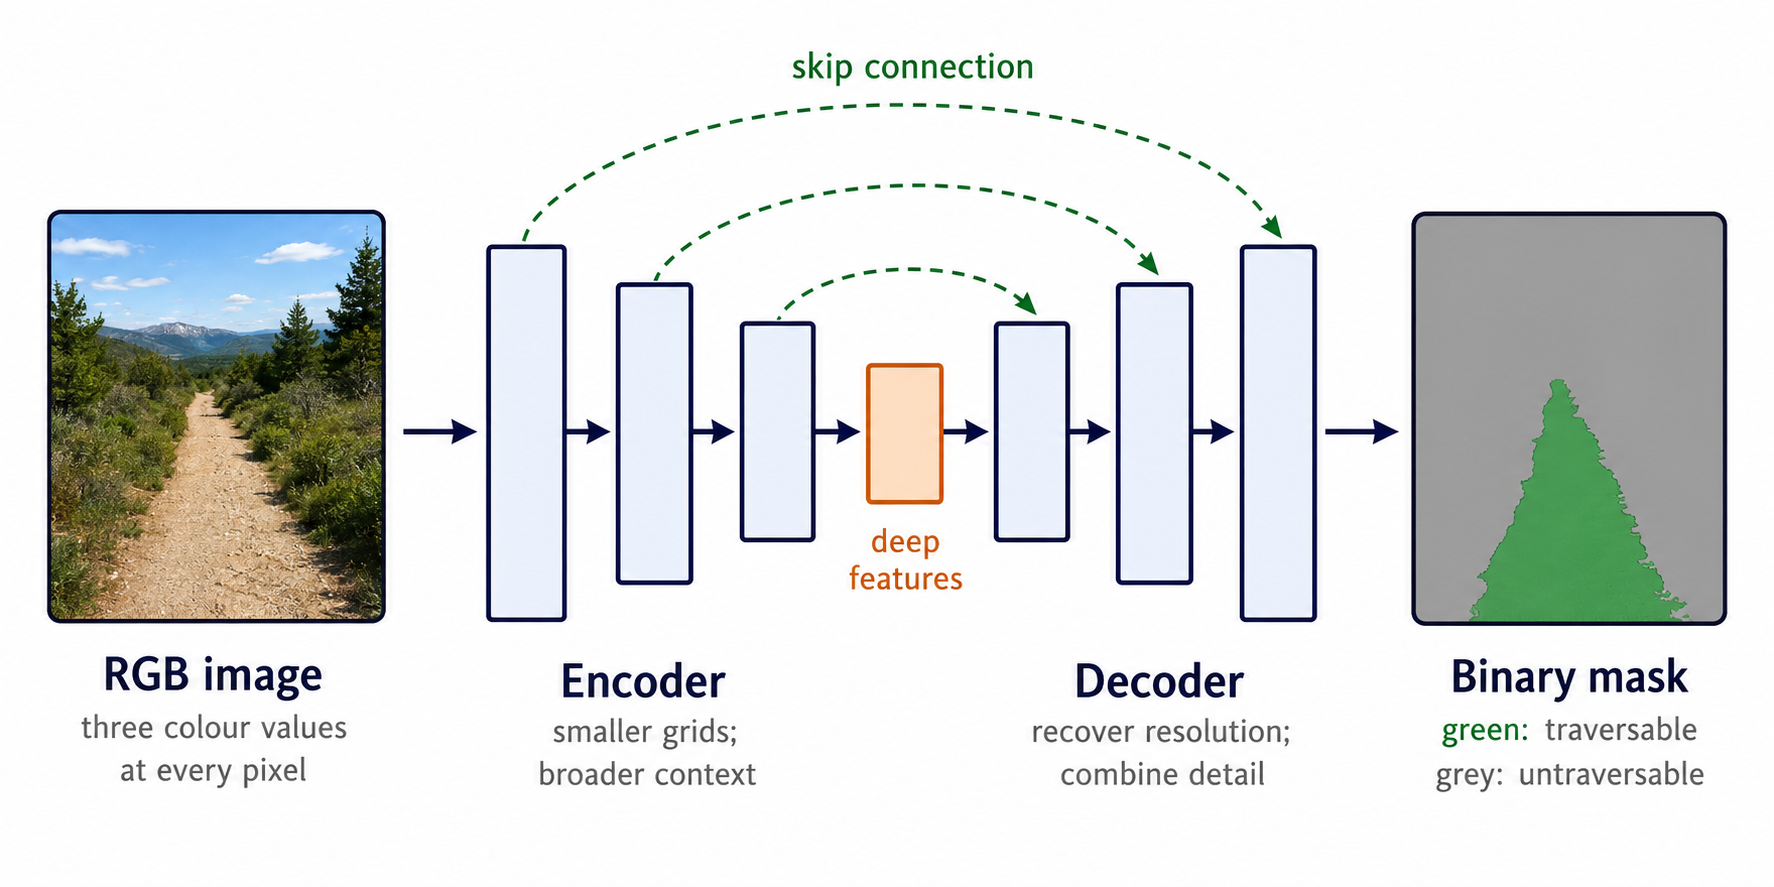
\includegraphics[width=\textwidth]{../fig2dash1.png}
\caption[From an RGB image to a binary segmentation mask.]{From an RGB image
to a binary segmentation mask. The encoder gathers increasingly broad context,
the decoder restores spatial resolution, and skip connections preserve local
detail. The landscape and mask are conceptual rather than dataset samples.
Original schematic drawn for this thesis.}
\label{fig:segmentation_concept}
\end{figure}

U-Net is a clear example of this pattern~\cite{ronneberger2015unet}. Its encoder
contracts the image representation in several stages, and its approximately
symmetric decoder expands it again. At each scale, a skip connection provides
the decoder with encoder features of the same resolution. U-Net was introduced
for biomedical images, where accurate boundaries are important, but the same
design principle is useful for roads, terrain, and many other segmentation
tasks.

Feature Pyramid Networks (FPNs) organise the same multi-scale idea
differently~\cite{lin2017fpn}. The encoder first produces a hierarchy of
features: fine features near the input and coarser, more semantic features
deeper in the network. A top-down path then carries semantic information back
towards the finer resolutions. Lateral connections join the top-down signal
with the encoder feature at each scale. The result is a pyramid in which
several resolutions contain useful semantic information. Although FPN was
introduced for object detection, this pyramid is also a practical decoder for
segmentation.

\subsection{Learning Context at More Than One Scale}

An object or terrain region does not have one fixed size in the image. Nearby
stones may occupy many pixels; the same stones in the distance may occupy only
a few. Segmentation systems therefore need to combine information gathered at
different spatial scales.

PSPNet does this using pyramid pooling~\cite{zhao2017pspnet}. It pools a deep
feature map into several grid sizes. A very coarse grid summarises almost the
whole scene, while finer grids retain more local variation. The pooled results
are resized and combined, giving the prediction access to both global and
regional context. DeepLabv3+ uses another method, known as \emph{atrous} or
\emph{dilated} convolution~\cite{chen2018deeplab}. A dilated filter samples
positions that are spaced apart, allowing it to cover a wider area without
reducing the feature-map resolution by the same amount. DeepLabv3+ then adds a
decoder to refine boundaries.

These methods are not merely interchangeable names. They express different
engineering choices. Pooling summarises regions explicitly. Dilated
convolution widens the sampled neighbourhood. Skip-connected decoders recover
detail from earlier layers. Multi-resolution networks, discussed below, keep
more than one resolution active throughout much of the model. Each choice
changes memory use, computation, and the type of spatial evidence that reaches
the final classifier.

\subsection{What the Network Produces in This Thesis}

The final layer produces one numerical score, or \emph{logit}, for each class
at each pixel. A logit is an unnormalised confidence value. During training,
the logits are compared with the annotated mask by a loss function. The loss
is a single number that measures how incompatible the prediction is with the
target; optimisation changes the network weights to reduce it. During
evaluation, the class with the stronger output is selected, or an equivalent
probability threshold is applied for the binary decision.

For CaT, the target is not a material map. The positive class is defined by a
vehicle-capability policy described in Chapter~\ref{ch:cat_pipeline}. A pixel
showing grass can be positive in one place and negative in another if the
annotation indicates different vehicle access. The network is thus learning a
visual approximation of the released capability labels, not a universal law
that grass, soil, or gravel is always safe.

The context--resolution trade-off has a direct meaning here. The model should
recognise that a partly shadowed surface continues as one track, which requires
scene context. At the same time, it should place the border between that track
and adjacent vegetation accurately, which requires local detail. A large open
region contributes many pixels to an average score, while a thin but
safety-relevant boundary contributes relatively few. This is why the thesis
examines not only overall overlap but also false-safe, false-block, and boundary
errors.

\section{Compact Encoders and Real-Time Architectures}

\subsection{Why Compact Models Matter}

An autonomous vehicle receives a continuous stream of camera frames. A useful
model must finish processing one frame before too many new frames arrive.
Otherwise the perception result describes an increasingly old scene. Large
models may achieve high accuracy on a server but be unsuitable for a vehicle
with limited processing power, memory, electrical power, or cooling.

The word \emph{compact} can describe several different properties. A model may
have few learned parameters, require few arithmetic operations, use little
temporary memory, or run quickly on a particular processor. These properties
are related but not identical. Parameters are the learned numerical weights
stored by the model. Operation counts estimate arithmetic work. Latency is the
time actually required to process a frame. A model with fewer parameters can
still be slower if its operations are poorly supported by the hardware or if
it repeatedly moves large feature maps through memory.

This thesis therefore treats compact architecture design and measured runtime
as separate questions. Architecture explains why a model might be efficient.
Timing experiments later determine whether that expectation holds on the CPU,
H100 partition, and RTX~5060 systems that were actually used.

\subsection{MobileNetV2: Reducing the Cost of Convolution}

A standard convolution learns filters that jointly combine spatial positions
and input channels. This is powerful but can be expensive. A
\emph{depthwise-separable convolution} divides the work into two steps. First,
a small spatial filter is applied independently to each channel. Second, a
$1\times1$ convolution mixes information across channels. The factorisation
usually requires much less computation than one dense convolution with a
similar input and output size.

Figure~\ref{fig:depthwise_convolution} shows the factorisation without relying
on operation-count notation. A standard convolution performs spatial filtering
and channel mixing together. The depthwise-separable alternative first asks
where a pattern occurs inside each channel and then uses a $1\times1$ operation
to combine the channel responses.

\begin{figure}[H]
\centering
\resizebox{\textwidth}{!}{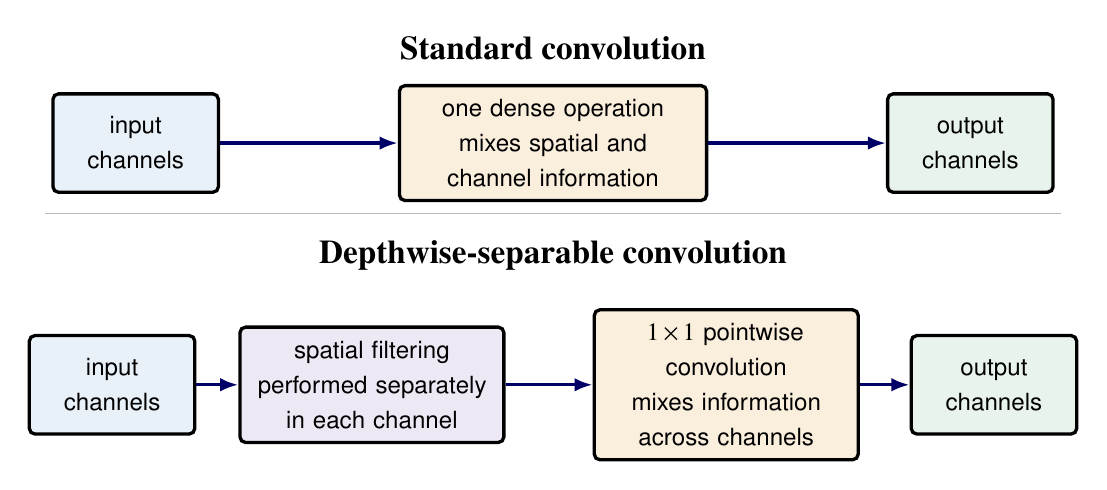
\begin{tikzpicture}[
  font=\sffamily\small,
  block/.style={draw,rounded corners=2pt,very thick,align=center,
    minimum height=1.25cm,inner sep=5pt},
  flow/.style={-{Latex[length=2.3mm]},very thick,draw=azulUC3M},
  note/.style={align=center,font=\footnotesize,text=black!78}
]
  \node[font=\bfseries\large] at (6.55,5.05) {Standard convolution};
  \node[block,fill=softblue,text width=1.75cm] (sin) at (1.25,3.85)
    {input\\channels};
  \node[block,fill=softorange,text width=3.55cm] (sdense) at (6.55,3.85)
    {one dense operation mixes spatial and channel information};
  \node[block,fill=softgreen,text width=1.75cm] (sout) at (11.85,3.85)
    {output\\channels};
  \draw[flow] (sin) -- (sdense);
  \draw[flow] (sdense) -- (sout);

  \draw[black!28] (0.10,2.95) -- (13.00,2.95);

  \node[font=\bfseries\large] at (6.55,2.42) {Depthwise-separable convolution};
  \node[block,fill=softblue,text width=1.75cm] (din) at (0.95,0.78)
    {input\\channels};
  \node[block,fill=softpurple,text width=3.00cm] (depth) at (4.25,0.78)
    {spatial filtering\\performed separately\\in each channel};
  \node[block,fill=softorange,text width=3.00cm] (point) at (8.75,0.78)
    {$1\!\times\!1$ pointwise convolution\\mixes information\\across channels};
  \node[block,fill=softgreen,text width=1.75cm] (dout) at (12.15,0.78)
    {output\\channels};
  \draw[flow] (din) -- (depth);
  \draw[flow] (depth) -- (point);
  \draw[flow] (point) -- (dout);
\end{tikzpicture}
}
\caption[Standard and depthwise-separable convolution.]{Conceptual difference
between a standard convolution and a depthwise-separable convolution. Splitting
spatial filtering from channel mixing is the main efficiency mechanism used by
MobileNetV2. Original schematic drawn for this thesis.}
\label{fig:depthwise_convolution}
\end{figure}

MobileNetV2 was designed around this idea for resource-constrained
devices~\cite{sandler2018mobilenetv2}. Its characteristic unit is the
\emph{inverted residual block}. The block first expands a narrow input into
more channels, applies an inexpensive depthwise spatial convolution, and then
projects the result back into a narrow representation. It is ``inverted''
because the wider representation exists inside the block rather than between
blocks, which is the opposite of the bottleneck pattern used in many earlier
residual networks.

The final projection is linear: it does not apply the usual nonlinear
activation after compressing the feature. MobileNetV2 calls this a
\emph{linear bottleneck}. The motivation is that forcing a nonlinear
operation onto a very narrow representation can destroy useful information.
When the input and output shapes match, a residual connection also lets the
block add its input to its output. This gives information and gradients a
shorter path through the network.

In this thesis, MobileNetV2 is used as an encoder rather than as a complete
image classifier. Intermediate features from several resolutions are passed to
an FPN or U-Net decoder. This pairing asks a concrete question: when the
decoder is held fixed, how well does a highly economical encoder preserve the
evidence needed for CaT segmentation?

\subsection{EfficientNet-B0: Balancing Width, Depth, and Image Resolution}

There are three common ways to make a CNN larger. It can be made
\emph{deeper} by adding layers, \emph{wider} by adding channels to each layer,
or it can process a higher-resolution image. Increasing only one dimension can
produce an unbalanced model. For example, a very deep but narrow network may
have limited feature capacity, while a wide network operating on a small image
cannot recover detail that the resizing step removed.

EfficientNet introduced a compound scaling method that increases depth, width,
and input resolution together using a coordinated rule
~\cite{tan2019efficientnet}. EfficientNet-B0 is the baseline architecture from
which the larger EfficientNet variants are scaled. Its building blocks also
use efficient depthwise operations, but the overall channel sizes and stage
layout differ from MobileNetV2.

EfficientNet-B0 is relevant here for two reasons. First, it is still small
enough to be a plausible compact encoder. Second, pretrained weights are
widely available, so the model begins with visual features learned from a much
larger image collection than CaT. Pretraining does not mean that the network
already understands traversability. It means that the early and middle layers
already respond to broadly useful visual structures such as contours,
textures, and object parts. Training on CaT then adapts those features to the
binary target.

MobileNetV2 and EfficientNet-B0 are each paired with FPN and U-Net. This
$2\times2$ arrangement avoids changing the encoder and decoder at the same
time. MobileNetV2/FPN can be compared with EfficientNet-B0/FPN to isolate the
encoder choice approximately. MobileNetV2/FPN can be compared with
MobileNetV2/U-Net to examine the decoder choice while retaining the same
encoder. It is a limited comparison rather than a universal proof, because
training details and implementation quality can still interact with each
architecture.

\subsection{Networks Designed Specifically for Real-Time Segmentation}

General encoder--decoder models reduce an image and reconstruct it afterwards.
Real-time segmentation research has also explored architectures that preserve
a high-resolution route for longer.

BiSeNetV2 uses two branches~\cite{yu2021bisenetv2}. The detail branch remains
comparatively wide and shallow so that it retains edges and fine spatial
structure. The semantic branch reduces resolution more aggressively so that
it can recognise scene-level meaning at lower computational cost. A guided
aggregation layer combines the branches rather than simply adding their
outputs. In plain terms, one route concentrates on \emph{where} boundaries
are, the other on \emph{what} the regions mean, and the fusion stage learns
how much to use from each.

DDRNet, or Deep Dual-Resolution Network, also keeps two resolutions active
~\cite{hong2022ddrnet}. A low-resolution branch can be deep and gather broad
context efficiently. A high-resolution branch preserves spatial precision.
Repeated bilateral exchanges pass information in both directions: coarse
semantic information is resized and supplied to the detailed branch, while
detailed information is reduced and supplied to the coarse branch. The
23-Slim variant included in this thesis is the smaller, throughput-oriented
member of the family.

SegFormer provides a different comparison because its encoder is based on a
vision transformer rather than only on convolution~\cite{xie2021segformer}.
A transformer represents an image as a sequence of feature tokens and uses
\emph{attention} to let one token gather information from other locations.
This can connect distant parts of the image without relying only on a long
chain of local convolutional filters. SegFormer's Mix Transformer is
hierarchical: it progressively reduces resolution and produces features at
several scales, much like a CNN pyramid. A lightweight multilayer-perceptron
(MLP) decoder projects and combines these features. Here, an MLP is a small
set of learned channel-mixing layers, not a second large image-processing
network.

PIDNet is the third multi-resolution family in the comparison. It retains
separate routes for detail, context, and boundaries. Because PIDNet-S is the
initial model developed in this thesis, its design is explained separately in
Section~\ref{sec:pidnet_background}.

None of these descriptions establishes which network is fastest. Attention,
depthwise convolution, multi-branch exchange, and high-resolution features
produce different patterns of arithmetic and memory access. CPUs, general
GPUs, and TensorRT may optimise those patterns differently. Consequently, the
later hardware chapter reports measured latency under a stated timing scope
instead of converting parameter counts into assumed speed.

Table~\ref{tab:architecture_families} groups the model families later compared
and identifies the principal design contrast represented by each one.

\begin{table}[H]
\centering
\caption{Architecture families, implemented systems, and the principal design
contrast represented in the comparative experiment.}
\label{tab:architecture_families}
\small
\begin{tabularx}{\textwidth}{@{}
  >{\raggedright\arraybackslash}p{0.23\textwidth}
  >{\raggedright\arraybackslash}p{0.31\textwidth}
  >{\raggedright\arraybackslash}X@{}}
\toprule
\textbf{Family} & \textbf{Systems in this thesis} & \textbf{Main design question represented} \\
\midrule
General encoder--decoder & FPN and U-Net with MobileNetV2 or EfficientNet-B0 & How encoder capacity and decoder organisation affect the common task \\
Multi-resolution real-time CNN & PIDNet-S, DDRNet-23-Slim, BiSeNetV2 & Whether explicit detail/context streams provide a better speed--accuracy balance \\
Compact task-specific transformer & SegFormer-B0 & Whether hierarchical attention with a light decoder improves context efficiently \\
Frozen foundation-model transfer & ROD ViT-S & Whether pretrained EfficientSAM features transfer to CaT with only the decoder trained \\
\bottomrule
\end{tabularx}
\end{table}

\section{PIDNet-S}
\label{sec:pidnet_background}

\subsection{Why the Name Refers to a PID Controller}

PIDNet takes its name from proportional--integral--derivative (PID) control
~\cite{xu2023pidnet}. A traditional PID controller repeatedly compares a
desired value with a measured value. Its proportional term reacts to the
current error, its integral term accumulates error over time, and its
derivative term reacts to how quickly the error is changing. PIDNet does
\emph{not} place such a controller inside the segmentation model and it does
not operate over time in this thesis. The authors use the three roles as an
analogy for organising spatial image information.

The analogy addresses a known problem in segmentation. A deep,
low-resolution route is effective at understanding the overall scene but can
produce smooth, imprecise borders after it is enlarged. A high-resolution route
preserves location but may lack enough context to distinguish visually similar
regions. PIDNet adds a third, boundary-focused route instead of expecting one
feature stream to perform all three jobs.

\subsection{The Three Processing Branches}

PIDNet calls its branches P, I, and D:

\begin{itemize}
  \item The \textbf{P branch} is the proportional branch. It keeps a relatively
  high feature resolution and responds strongly to local appearance. Its main
  role is to preserve spatial detail: corners, narrow structures, and the
  position of region boundaries.
  \item The \textbf{I branch} is the integral branch. It follows a deeper,
  lower-resolution path and obtains a larger receptive field. Its main role is
  semantic context. It can use a wider view to decide whether a local texture
  belongs to a continuous track, vegetation, or background.
  \item The \textbf{D branch} is the derivative branch. It is trained to
  emphasise rapid spatial changes associated with semantic boundaries. Here,
  \emph{high frequency} means that feature values change sharply across nearby
  pixels, as they often do at an edge. The branch
  supplies an explicit cue about where one predicted region should end and
  another should begin.
\end{itemize}

The branches are not independent models. They exchange information at several
stages and are fused before the final mask is produced. This matters because a
boundary cue without semantic context cannot say which side is traversable,
while a semantic region without boundary evidence may spread too far.

\subsection{How Information Is Combined}

The Pixel-attention-guided Fusion Module (PagFM) transfers information from
the context-rich I branch to the detailed P branch. \emph{Attention} here
means a learned spatial weighting. The module compares features and computes
where the semantic information should be trusted. It can then add useful
context without replacing the high-resolution representation everywhere.

Near the end of PIDNet-S, the Parallel Aggregation Pyramid Pooling Module
(PAPPM) collects context at several scales. Like other pyramid-pooling
methods, it creates summaries over differently sized regions. The parallel,
lightweight construction is intended to provide a broad scene view without
turning the small model into a heavy decoder.

The final combination uses Light-Bag, the lightweight form of the
Boundary-attention-guided fusion module. Boundary information from the D
branch guides the combination of detailed and semantic features. Away from a
boundary, the model can favour stable region-level context. Near a boundary,
it can give more importance to the representation that preserves local
structure. The exact weights are learned during training rather than defined
by a hand-written rule.

\subsection{Why PIDNet-S Is the Starting Point}

The suffix ``S'' identifies the small PIDNet variant. The implementation used
here has 7.62 million parameters. It was selected as the first model because
the CaT task contains the three visual demands represented by its branches:
broad trail context, small irregular details, and capability boundaries that
matter to the safety interpretation. Its size also made repeated development
experiments practical and provided a plausible route to CPU and embedded-GPU
deployment.

This motivation is a hypothesis, not a result. A specialised boundary branch
does not guarantee the best CaT score, and a low parameter count does not
guarantee the lowest latency. Chapters~\ref{ch:pidnet} and
\ref{ch:results} therefore separate the architectural rationale from the
measured outcome. PIDNet-S first establishes the dataset, loss, checkpoint,
threshold, and evaluation pipeline. The later controlled study then compares
it with conventional encoder--decoder networks, other real-time CNNs, a compact
transformer, and ROD.

\section{ROD and Frozen-Encoder Transfer}

\subsection{Why Pretraining Is Useful on a Small Dataset}

Training a neural network begins by adjusting its weights from an initial
state. If the initial weights are random, the model must learn both basic
visual patterns and the final task from the available training images. CaT is
small compared with the large datasets commonly used in computer vision. A
high-capacity network can therefore memorise details of the training set
instead of learning features that transfer to new scenes.

\emph{Pretraining} addresses this problem by starting from weights learned on
a larger source task. The source task need not use the same labels. Edges,
repeated textures, object contours, and relationships between image regions
can remain useful when the final label changes from an object category to
traversability. The final model then performs \emph{transfer learning}: it
transfers a general visual representation and learns a smaller task-specific
mapping for CaT.

There are two broad ways to use a pretrained encoder. Fine-tuning continues to
update some or all encoder weights on the new task. Freezing keeps those
weights fixed and trains only newly attached layers. Fine-tuning gives the
encoder more freedom to adapt but also increases the risk of overfitting or
damaging useful pretrained features. Freezing reduces that risk and lowers the
memory required to store gradients during training, but it prevents the
encoder from correcting a representation that is poorly matched to the new
domain.

The two-stage process is illustrated in
Figure~\ref{fig:frozen_transfer_learning}. Pretraining learns the encoder on a
large source corpus. For the CaT task, ROD copies those weights, keeps them
fixed, and updates only the decoder that converts the retained features into a
traversability mask.

\begin{figure}[H]
\centering
\resizebox{0.95\textwidth}{!}{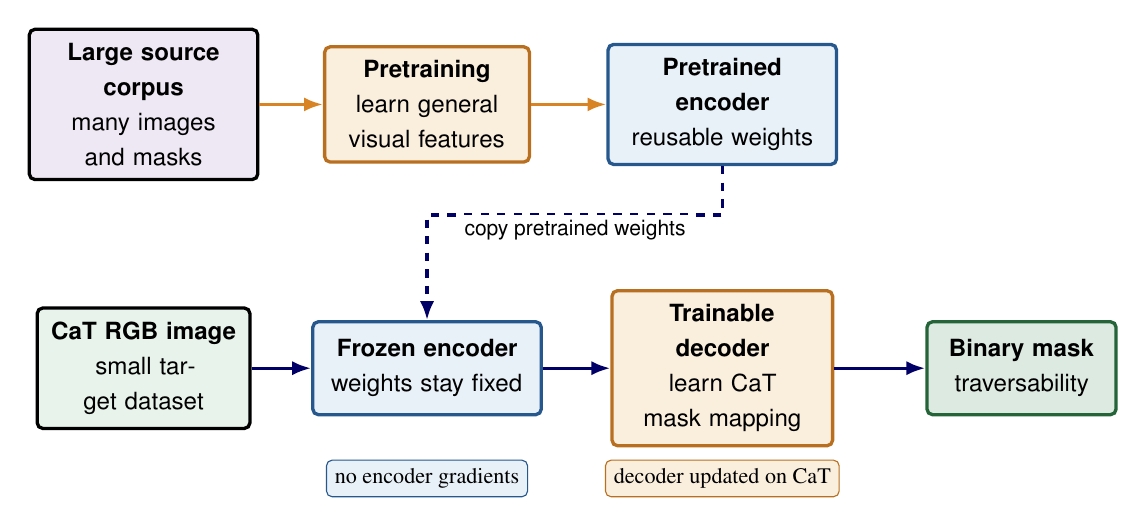
\begin{tikzpicture}[
  font=\sffamily\small,
  block/.style={draw,rounded corners=2pt,very thick,align=center,
    minimum height=1.18cm,inner sep=5pt},
  flow/.style={-{Latex[length=2.4mm]},very thick,draw=azulUC3M},
  trainflow/.style={-{Latex[length=2.4mm]},very thick,draw=warn},
  fixed/.style={block,draw=pidP!80!black,fill=softblue},
  trainable/.style={block,draw=warn!85!black,fill=softorange}
]
  \node[block,fill=softpurple,text width=2.55cm] (source) at (1.4,3.65)
    {\textbf{Large source corpus}\\many images and masks};
  \node[trainable,text width=2.25cm] (pretrain) at (5.0,3.65)
    {\textbf{Pretraining}\\learn general visual features};
  \node[fixed,text width=2.55cm] (weights) at (8.75,3.65)
    {\textbf{Pretrained encoder}\\reusable weights};
  \draw[trainflow] (source) -- (pretrain);
  \draw[trainflow] (pretrain) -- (weights);

  \node[block,fill=softgreen,text width=2.35cm] (cat) at (1.4,0.30)
    {\textbf{CaT RGB image}\\small target dataset};
  \node[fixed,text width=2.55cm] (frozen) at (5.0,0.30)
    {\textbf{Frozen encoder}\\weights stay fixed};
  \node[trainable,text width=2.45cm] (decoder) at (8.75,0.30)
    {\textbf{Trainable decoder}\\learn CaT mask mapping};
  \node[block,fill=good!16,draw=good!80!black,text width=2.05cm] (mask) at (12.55,0.30)
    {\textbf{Binary mask}\\traversability};
  \draw[flow] (cat) -- (frozen);
  \draw[flow] (frozen) -- (decoder);
  \draw[flow] (decoder) -- (mask);
  \draw[flow,dashed] (weights.south) -- ++(0,-0.62) -| (frozen.north);
  \node[font=\sffamily\footnotesize,fill=white,inner sep=2pt]
    at (6.88,2.05) {copy pretrained weights};

  \node[draw=pidP!80!black,fill=softblue,rounded corners=2pt,
    font=\footnotesize,inner sep=3pt] at (5.0,-1.10) {no encoder gradients};
  \node[draw=warn!85!black,fill=softorange,rounded corners=2pt,
    font=\footnotesize,inner sep=3pt] at (8.75,-1.10) {decoder updated on CaT};
\end{tikzpicture}
}
\caption[Frozen-encoder transfer learning used by ROD.]{Frozen-encoder transfer
learning used by ROD. Blue blocks retain pretrained weights; the orange
decoder is the part trained for the CaT target. Freezing changes training, but
the encoder still executes for every image. Original schematic drawn for this
thesis.}
\label{fig:frozen_transfer_learning}
\end{figure}

\subsection{From Vision Transformers to EfficientSAM}

A vision transformer divides an image representation into a grid of
\emph{tokens}. A token is a feature vector describing one image patch or one
location in an intermediate feature map. Attention allows each token to build
a weighted combination of information from other tokens. In principle, a
location on one side of a track can therefore use evidence from a distant
continuation of that track directly~\cite{dosovitskiy2021vit}.

The benefit comes with a cost. Comparing many token pairs can be expensive,
especially when the spatial grid is large. Efficient transformer designs
reduce token resolution, use hierarchical stages, or otherwise simplify the
attention computation. EfficientSAM is an efficient segmentation model whose
encoder is trained to retain useful representations for mask prediction
~\cite{xiong2024efficientsam}. The ViT-S name used here means the small vision
transformer variant; ``small'' is relative to larger transformer variants and
does not mean that its deployment cost is negligible.

EfficientSAM belongs to the broader family of promptable segmentation models
popularised by the Segment Anything Model~\cite{kirillov2023sam}. Such models
are designed to produce masks using guidance such as points or boxes. ROD does
not use EfficientSAM as an interactive tool. It reuses the
pretrained image encoder as a source of multi-scale visual features and learns
a decoder for automatic off-road freespace prediction.

\subsection{What ROD Changes}

ROD stands for RGB-Only Fast and Efficient Off-road Freespace Detection
~\cite{sun2025rod}. Earlier multimodal freespace approaches can use RGB
appearance together with geometry derived from LiDAR. LiDAR measures distance
using emitted light and can provide a three-dimensional point cloud. Surface
normals derived from that geometry describe local surface orientation, which
helps identify slopes and obstacles. The cost is an additional sensor,
calibration between camera and LiDAR, synchronisation, and a more complex
processing chain.

ROD removes the LiDAR-derived branch and predicts from RGB alone. Its
EfficientSAM ViT-S encoder remains frozen. A convolutional decoder reads
features from more than one encoder scale, combines them, and learns the target
mask. ``RGB-only'' therefore describes the sensor input, not a claim that the
model is a small CNN. Every image still passes through the complete transformer
encoder.

\subsection{How ROD Is Used in This Thesis}

ROD is relevant because it represents a different strategy from PIDNet-S.
PIDNet-S trains a purpose-built compact segmentation network on CaT. ROD
retains a larger pretrained representation and trains only the decoder. The
comparison asks whether strong frozen features compensate for the small
dataset, and what runtime cost accompanies that transfer.

Freezing reduces the number of \emph{trainable} parameters, but not necessarily
the number of operations at inference. Gradients are unnecessary during
deployment, yet the encoder must still calculate its feature maps for every
frame. A frozen transformer can therefore be economical to train and still be
slower than a fully trainable compact CNN at runtime.

The published ROD result and RTX~A6000 timing cannot be copied directly into a
CaT comparison. The dataset, target definition, hardware, software, and timer
scope differ. In addition, the publication does not specify every item needed
to recreate its training run, including the epoch budget, augmentation policy,
and complete timing procedure. Chapter~\ref{ch:rod_extension} consequently
describes the implementation in this thesis as a reconstructed ROD
configuration. Documented elements are retained, missing choices are stated,
and the model is evaluated through the same CaT split and metric code as the
other architectures.

\section{CaT Literature and Comparability}

\subsection{Why Two Results From CaT May Still Measure Different Tasks}

Using the same dataset name does not make two headline scores directly
comparable. The studies must also agree on which pixels belong to each class,
which images are used for training and testing, how predictions are resized,
and how the final metric is calculated.

Intersection over Union (IoU) measures the overlap between a predicted region
and its target. The intersection contains pixels included in both regions. The
union contains pixels included in either region. Mean IoU (mIoU) averages class
IoUs. If four classes are replaced by two merged classes, both the regions and
the terms being averaged change. A four-class mIoU is therefore not a harder
or easier version of exactly the same number; it is a metric for a different
label space.

The distinction is especially important in CaT. Its colour-coded regions
represent nested vehicle capability. A blue-only binary policy asks whether a
sedan can traverse a pixel. A blue+green policy also accepts the pickup region.
A policy that merges blue, green, and red asks whether any represented vehicle
can traverse the pixel. All three policies use CaT, but a positive prediction
has a different physical meaning in each one.

\subsection{The Original Four-Class CaT Evaluation}

The original CaT study evaluates the four released classes separately using
PSPNet with several ResNet encoders
~\cite{sharma2022cat,zhao2017pspnet,he2016resnet}. ResNet introduced residual
connections that let a block learn a change relative to its input rather than
an entirely new representation. The numbered variants contain different
depths; a deeper backbone generally has more capacity and computation.

PSPNet then adds multi-scale pooled context to the backbone features before
producing the segmentation. Table~\ref{tab:cat_original_literature} reproduces
the reported test IoUs. The table is useful for showing that the released
images support strong pixel-level prediction and for identifying the
difficulty of individual capability bands. It is not a binary leaderboard for
the experiments in this thesis.

\begin{table}[H]
\centering
\caption{Original four-class CaT test results reported by Sharma et al.\
\cite{sharma2022cat}; values are percentages.}
\label{tab:cat_original_literature}
\small
\begin{tabular}{@{}llrrrrr@{}}
\toprule
\textbf{Network} & \textbf{Backbone} & \textbf{Background} & \textbf{Sedan} & \textbf{Pickup} & \textbf{Off-road} & \textbf{mIoU} \\
\midrule
PSPNet & ResNet-18  & 94.60 & 90.44 & 66.62 & 79.71 & 82.84 \\
PSPNet & ResNet-34  & 94.79 & 91.22 & 68.65 & 80.52 & 83.79 \\
PSPNet & ResNet-50  & 94.63 & 90.70 & 67.40 & 80.00 & 83.18 \\
PSPNet & ResNet-101 & 95.00 & 91.65 & 69.08 & 81.00 & 84.18 \\
\bottomrule
\end{tabular}
\end{table}

\subsection{EfficientViT Results and Split Independence}

Faykus et al. evaluate an EfficientViT architecture on CaT and report a
98.22\% sedan IoU and a 94.44\% mean over the three traversability classes
~\cite{efficientvit_offroad}. EfficientViT is a vision-transformer family
designed to reduce the cost of attention. The architecture is relevant to
compact off-road perception, but the published CaT data accounting prevents a
direct ranking against this thesis.

The paper describes 3,624 images. The public release audited here contains
1,812 underlying images, with each sample accessible twice: once through its
environment folder and once through the consolidated \texttt{mixed} folder.
Thus, counting file paths instead of underlying samples also produces 3,624.
The reported train and test counts do not sum to the stated total, and no list
of sample identifiers is published for either partition.

This does not prove that training and test images overlap. It means that
independence cannot be checked. If two paths to the same underlying image were
placed in different partitions, the model could be evaluated on pixels it had
already seen during training. Because the identifiers are unavailable, this
thesis records the uncertainty and does not assign a cause or reconstruct the
authors' split.

\subsection{Binary CaT With a Different Positive Class}

Ramtekkar et al. formulate CaT as a binary road-detection task
~\cite{ramtekkar2024depth}. However, they merge the sedan, pickup, and
off-road-only regions into the positive road class. Their positive region is
therefore broader than either binary policy studied here.

Their system uses the MiT-B3 encoder from the SegFormer family and contains
approximately 64 million parameters. It is trained using a generated
multi-source corpus of 2.7 million images. This additional data can expose the
model to far more appearance variation than the CaT training partition alone.
The work answers a useful question about robust road-region detection, but it
does not isolate learning from the public CaT training set under a
sedan-oriented or pickup-inclusive policy.

The reported road IoU should consequently not be placed beside the mIoU values
in Chapter~\ref{ch:results} as though the models took the same examination.
The class definition, training corpus, architecture scale, and metric differ.

Table~\ref{tab:comparability} collects these protocol differences and states
which kinds of comparison remain valid.

\begin{table}[H]
\centering
\caption{Why headline CaT results require protocol alignment before comparison.}
\label{tab:comparability}
\small
\begin{tabularx}{\textwidth}{@{}
  >{\raggedright\arraybackslash}p{0.23\textwidth}
  >{\raggedright\arraybackslash}p{0.24\textwidth}
  >{\raggedright\arraybackslash}X@{}}
\toprule
\textbf{Study} & \textbf{Target} & \textbf{Principal comparability issue} \\
\midrule
Sharma et al.~\cite{sharma2022cat} & Four mutually exclusive raw labels encoding vehicle-capability bands & Four-class optimisation and mIoU differ from merged binary evaluation \\
Faykus et al.~\cite{efficientvit_offroad} & Three traversability-class mean & Published sample counts and absent manifest do not establish an independent split \\
Ramtekkar et al.~\cite{ramtekkar2024depth} & Blue+green+red as road & Different positive class and much larger generated training corpus \\
This thesis & Blue-only or blue+green binary & Official test retained; exact binary policy, split, seeds, and artifacts declared \\
\bottomrule
\end{tabularx}
\end{table}

\subsection{The Comparison Rule Used Here}

Only the sedan IoU from the original four-class study uses the same positive
pixel set as the blue-only traversable IoU. Even that number is not fully
equivalent: the original network must distinguish all four classes during
training, whereas the binary network only separates traversable from
untraversable.

The literature is therefore used in two ways. First, it explains how CaT has
been interpreted by previous systems. Second, it identifies protocol choices
that must be stated for a reproducible comparison. Numerical ranking is
reserved for models evaluated here with the same binary mask policy, split
manifest, evaluator, and timing definition. This narrower rule produces fewer
headline comparisons, but the remaining comparisons have a clear meaning.

\section{Research Gap}

The background above leads to four practical gaps. Each gap is expressed here
as a question that the experimental chapters can answer.

\subsection{What Does ``Traversable'' Mean?}

CaT does not provide one universal road class. It provides nested regions for
vehicles with different capabilities. A result has little operational meaning
unless it states which of those regions are treated as positive. This thesis
therefore defines two explicit binary policies and makes the blue+green policy
the principal one. Every reported experiment names its policy.

\subsection{What Kind of Mistake Did the Model Make?}

One mIoU value combines several outcomes. For navigation, predicting an
untraversable pixel as traversable is qualitatively different from blocking a
pixel that was actually traversable. The first error can make terrain labelled
untraversable available to the planner;
the second can remove a valid route and make the vehicle unnecessarily
conservative. This thesis reports False-Safe Rate and False-Block Rate
alongside overlap metrics, and it inspects where those errors occur in the
image.

\subsection{Is a Model Fast on the Hardware That Will Run It?}

Published frames-per-second values often use different processors, input
sizes, numeric precision, batch sizes, and timer boundaries. One measurement
may time only the neural-network forward pass, while another includes image
preparation and transfer to the GPU. The resulting numbers are not
interchangeable. This thesis measures the selected models on declared hardware
and states exactly which operations each timer includes.

\subsection{Can the Result Be Traced and Repeated?}

A checkpoint alone does not describe an experiment. Reproduction also needs
the file partition, label conversion, image size, preprocessing, training
configuration, selection rule, threshold, and evaluation code. The work
therefore saves manifests, configurations, checkpoints, metric outputs, and
timing records as linked artifacts.

These gaps explain why the thesis does more than introduce another
segmentation network. Its contribution is a common, inspectable experiment in
which compact architectures are trained for the same vehicle-level task,
evaluated with both accuracy and safety-oriented measures, and timed under
declared deployment conditions. Chapter~\ref{ch:cat_pipeline} next defines the
data and label pipeline on which that comparison depends.

% ============================================================
\chapter{CaT Binary Task and Common Pipeline}
\label{ch:cat_pipeline}
% ============================================================

\section{Dataset Release and Audit}

The first implementation task was not model training but establishing what the
dataset actually contains. The CaT release~\cite{sharma2022cat} exposes each underlying sample in
an environment-specific directory and again in a consolidated
\texttt{mixed} directory. Treating both directory views as independent images
would double the nominal sample count and could place identical scenes in
different partitions. The pipeline therefore consumes only the consolidated
tree and treats the environment folders as alternate views useful for audit.

The release contains Brown Field, Main Trail, and Power Line environments.
Their cameras and stored image resolutions are not uniform. Brown Field images
are $1024\times644$, Main Trail images are $960\times604$, and Power Line
contains both $720\times452$ and $1920\times1208$ images. Table
~\ref{tab:cat_environment_counts} gives the exact release counts. The
Power Line environment contributes 78.5\% of the data, so an aggregate test
score is influenced more strongly by its appearance distribution than by the
two smaller environments.

\begin{table}[H]
\centering
\caption{Audited CaT environment counts and stored RGB resolutions.}
\label{tab:cat_environment_counts}
\small
\begin{tabularx}{\textwidth}{@{}lrrrX@{}}
\toprule
\textbf{Environment} & \textbf{Train release} & \textbf{Test release} & \textbf{Total} & \textbf{Stored resolution(s)} \\
\midrule
Brown Field & 140 & 60 & 200 & $1024\times644$ \\
Main Trail & 133 & 57 & 190 & $960\times604$ \\
Power Line & 995 & 427 & 1,422 & $720\times452$; $1920\times1208$ \\
\midrule
Consolidated unique total & 1,268 & 544 & 1,812 & all of the above \\
\bottomrule
\end{tabularx}
\end{table}

For every consolidated sample, the audit pairs three files by numeric sample
identifier:
\begin{enumerate}
  \item the RGB PNG in \texttt{imgs};
  \item the coloured palette mask in \texttt{masks};
  \item the integer label map in \texttt{annos/int\_maps}.
\end{enumerate}
The audit validates that the expected files are present, readable, and
spatially aligned. All 1,812 selected samples have an exact integer-map pair;
the palette-mask fallback exists in the implementation but is not used for the
processed datasets reported here. The audit confirms that the label maps
contain only the expected raw IDs $\{0,1,2,3\}$ and that the palette masks use
only the four expected colours. It writes both a machine-readable report and
the discovered mapping configuration before any binary mask is generated.

This procedure was chosen over directly reading the colour masks during
training. Integer IDs are unambiguous and avoid dependence on PNG palette
interpretation. Retaining a validated colour fallback makes the tool robust to
a sample for which the integer map is absent, but silently mixing an
unaligned map with an image is forbidden.

\section{Vehicle-Capability Labels and Binary Policies}

CaT defines four nested capability regions:
\begin{itemize}
  \item raw ID 0, black $(0,0,0)$: background or untraversable;
  \item raw ID 1, blue $(27,122,235)$: sedan-traversable;
  \item raw ID 2, green $(56,162,4)$: additional pickup-traversable terrain;
  \item raw ID 3, red $(245,34,45)$: additional terrain reserved for the
  off-road vehicle.
\end{itemize}
The colours are annotation colours, not terrain appearances. ``Blue'' and
``green'' are therefore convenient policy names rather than physical surface
categories.

The main development policy merges sedan and pickup capability:
\begin{equation}
 y_{\mathrm{BG}} =
 \begin{cases}
 1,&r\in\{1,2\},\\
 0,&r\in\{0,3\},
 \end{cases}
 \label{eq:blue_green_mapping}
\end{equation}
Here, $r\in\{0,1,2,3\}$ is the raw CaT class ID and
$y_{\mathrm{BG}}\in\{0,1\}$ is the resulting binary label, with 1 denoting
traversable and 0 denoting untraversable. This policy asks whether a pixel lies inside the
combined sedan/pickup envelope. Raw off-road-only pixels are deliberately
blocked; calling every red pixel ``road'' would represent a more capable
vehicle and a different task.

\begin{figure}[H]
\centering
\resizebox{\textwidth}{!}{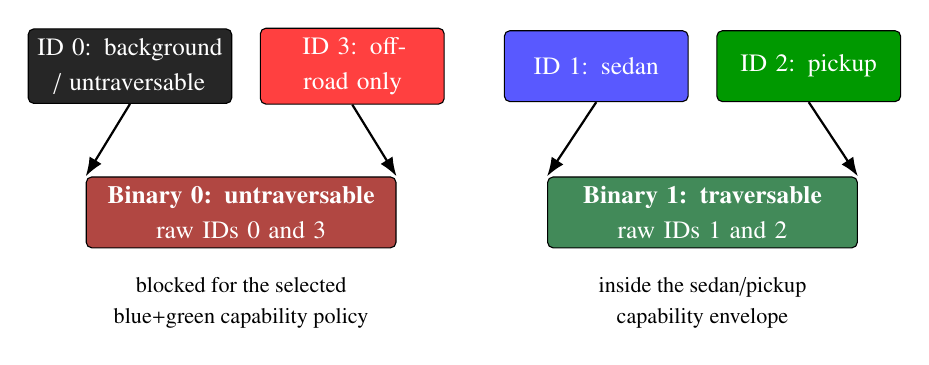
\begin{tikzpicture}[
  box/.style={draw,rounded corners=2pt,minimum height=0.9cm,align=center,font=\small},
  arrow/.style={-{Latex[length=2.4mm]},thick}
]
\node[box,fill=black!85,text=white,text width=2.35cm] (raw0) {ID 0: background / untraversable};
\node[box,fill=red!75,text=white,text width=2.1cm,right=0.35cm of raw0] (raw3) {ID 3: off-road only};
\node[box,fill=blue!65,text=white,text width=2.1cm,right=0.75cm of raw3] (raw1) {ID 1: sedan};
\node[box,fill=green!60!black,text=white,text width=2.1cm,right=0.35cm of raw1] (raw2) {ID 2: pickup};

\node[box,fill=safety!90,text=white,text width=3.7cm,below=1.4cm of $(raw0)!0.5!(raw3)$] (neg)
  {\textbf{Binary 0: untraversable}\\raw IDs 0 and 3};
\node[box,fill=good!90,text=white,text width=3.7cm,below=1.4cm of $(raw1)!0.5!(raw2)$] (pos)
  {\textbf{Binary 1: traversable}\\raw IDs 1 and 2};

\draw[arrow] (raw0.south) -- (neg.north west);
\draw[arrow] (raw3.south) -- (neg.north east);
\draw[arrow] (raw1.south) -- (pos.north west);
\draw[arrow] (raw2.south) -- (pos.north east);

\node[font=\footnotesize,align=center,below=0.25cm of neg] {blocked for the selected\\blue+green capability policy};
\node[font=\footnotesize,align=center,below=0.25cm of pos] {inside the sedan/pickup\\capability envelope};
\end{tikzpicture}
}
\caption[Conversion from CaT raw classes to the main binary policy.]{Conversion
from the four raw CaT classes to the main blue+green binary policy. The class
merge is a vehicle-capability decision, not a claim that the two merged raw
classes are visually or physically identical. Raw classes are grouped by
binary destination rather than numerical ID.}
\label{fig:cat_label_hierarchy}
\end{figure}

Figure~\ref{fig:cat_label_hierarchy} visualises how the four raw IDs enter the
two destination classes defined by Equation~\ref{eq:blue_green_mapping}.

The architecture experiment also evaluates a blue-only policy:
\begin{equation}
 y_{\mathrm{B}} =
 \begin{cases}
 1,&r=1,\\
 0,&r\in\{0,2,3\}.
 \end{cases}
 \label{eq:blue_only_mapping}
\end{equation}
Here, $y_{\mathrm{B}}\in\{0,1\}$ is the blue-only binary label, with 1
denoting traversable and 0 denoting untraversable; $r$ retains the raw-ID
definition above.
Blue-only is more conservative because pickup-only terrain is reassigned to
the blocked class. Its scores answer a different question from the blue+green
scores because the positive mask, class balance, and assumed vehicle all
change.

\begin{figure}[H]
\centering
\begin{subfigure}[t]{0.48\linewidth}
  \centering
  \includegraphics[width=\linewidth]{../CAT/mixed/Test/imgs/img_pln_1278.png}
  \caption{RGB input.}
\end{subfigure}\hfill
\begin{subfigure}[t]{0.48\linewidth}
  \centering
  \includegraphics[width=\linewidth]{../CAT/mixed/Test/masks/mask_pln_1278.png}
  \caption{Original four-colour CaT mask.}
\end{subfigure}

\vspace{0.25cm}
\begin{subfigure}[t]{0.48\linewidth}
  \centering
  
\includegraphics[width=\linewidth]{figures/generated/mixed_pln_1278_blue_only_display.png}
  \caption{Blue-only binary mask.}
\end{subfigure}\hfill
\begin{subfigure}[t]{0.48\linewidth}
  \centering
  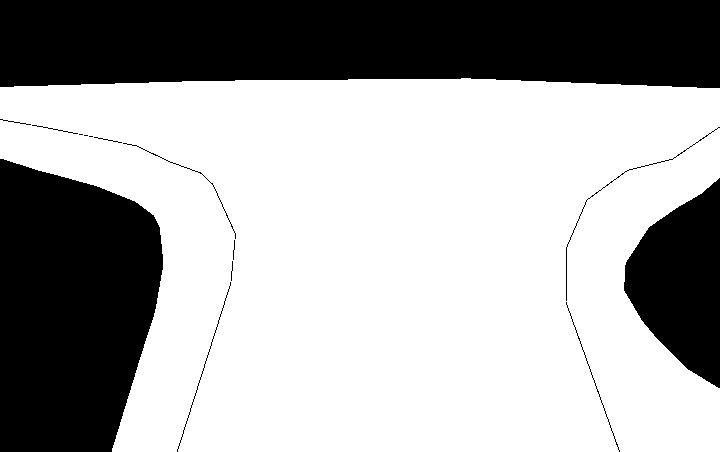
\includegraphics[width=\linewidth]{figures/generated/mixed_pln_1278_blue_green_display.png}
  \caption{Blue+green binary mask.}
\end{subfigure}
\caption[Example of the two binary conversions.]{Example of the two binary
conversions for \texttt{mixed\_pln\_1278}. In the lower masks, white denotes
traversable and black denotes untraversable. Blue-only retains the central raw
blue region; blue+green also admits the raw green shoulders. The upper raw red
field remains blocked in both policies.}
\label{fig:cat_binary_example}
\end{figure}

Figure~\ref{fig:cat_binary_example} also illustrates why the mapping must be
reported with every result. A binary visual can look plausible without
revealing whether green or red source regions were merged. The preprocessing
configuration therefore stores the traversable palette names and raw IDs, and
the processed summary records the mapping actually applied.

\section{Train, Validation, and Test Separation}

The original CaT test partition of 544 images is preserved intact and excluded
from gradient updates and automatic checkpoint selection. It is used for
read-only benchmark evaluation across several experiments, so it is not a
single-use blinded test set; Chapter~\ref{ch:protocols} states this limitation
explicitly. The original 1,268-image training partition is divided
into train and validation subsets by a deterministic hash:
\begin{equation}
 b(s)=
 \frac{
   \operatorname{int}\!\left(
   \operatorname{SHA256}\!\left(
     \operatorname{join}_{\texttt{:}}(\texttt{seed},\texttt{dataset},s)
   \right)_{0:12},16
   \right)}
 {16^{12}},
 \end{equation}
Here, $s$ is the complete sample identifier and $b(s)$ is its normalised hash
bucket, for which $0\leq b(s)<1$. The SHA-256 input is the UTF-8 string
$\operatorname{join}_{\texttt{:}}(\texttt{seed},\texttt{dataset},s)$, where
$\operatorname{join}_{\texttt{:}}$ concatenates the split seed, dataset name,
and complete sample identifier with colons. The subscript $0{:}12$ selects the
first 12 hexadecimal characters; $\operatorname{int}(\cdot,16)$ converts that
substring from base 16; division by $16^{12}$ normalises the integer to
$[0,1)$.
The sample is assigned to validation if $b(s)<0.2$. Split seed 1337 yields
1,002 training and 266 validation images. Hash bucketing makes the assignment
stable across machines and independent of filesystem ordering. It also
explains why the realised validation fraction is close to, but not exactly,
20\%.

Figure~\ref{fig:cat_data_partition} makes the information boundary explicit.
The validation set is created only from the official training part and is used
to select checkpoints. The official test branch remains outside optimisation
and automatic checkpoint selection, while repeated read-only evaluation is
shown as a separate benchmark path.

\begin{figure}[H]
\centering
\resizebox{0.94\textwidth}{!}{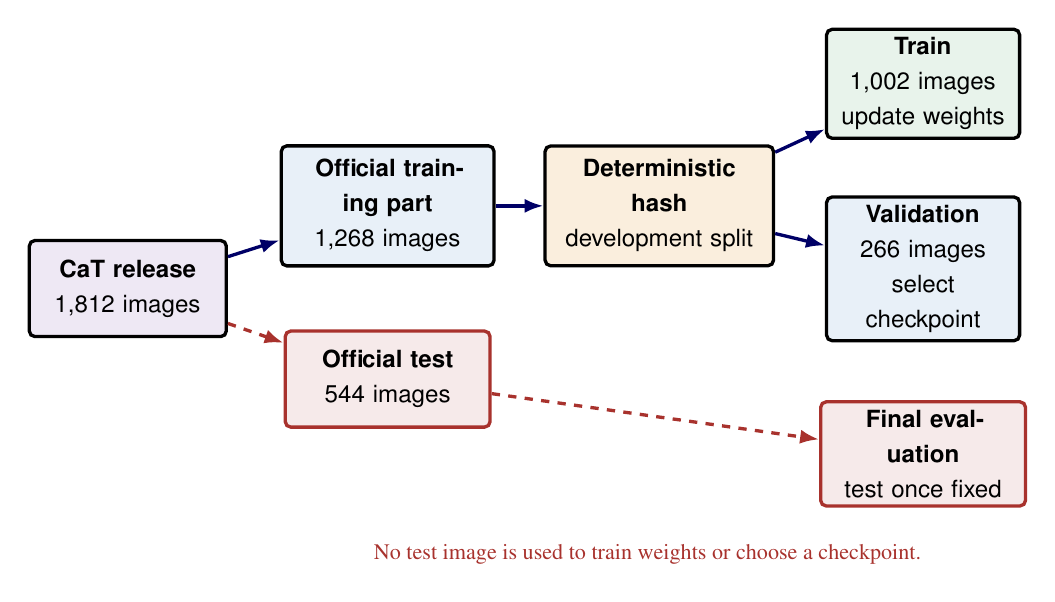
\begin{tikzpicture}[
  font=\sffamily\small,
  block/.style={draw,rounded corners=2pt,very thick,align=center,
    minimum height=1.22cm,inner sep=5pt},
  flow/.style={-{Latex[length=2.4mm]},very thick,draw=azulUC3M},
  sealed/.style={-{Latex[length=2.4mm]},very thick,dashed,draw=safety}
]
  \node[block,fill=softpurple,text width=2.15cm] (release) at (1.25,1.5)
    {\textbf{CaT release}\\1,812 images};
  \node[block,fill=softblue,text width=2.35cm] (dev) at (4.55,2.55)
    {\textbf{Official training part}\\1,268 images};
  \node[block,fill=safety!10,draw=safety,text width=2.25cm] (test) at (4.55,0.35)
    {\textbf{Official test}\\544 images};
  \node[block,fill=softorange,text width=2.55cm] (hash) at (8.0,2.55)
    {\textbf{Deterministic hash}\\development split};
  \node[block,fill=softgreen,text width=2.10cm,inner ysep=3pt] (train) at (11.35,4.10)
    {\textbf{Train}\\1,002 images\\update weights};
  \node[block,fill=softblue,text width=2.10cm,inner ysep=3pt] (val) at (11.35,1.75)
    {\textbf{Validation}\\266 images\\select checkpoint};
  \node[block,fill=safety!10,draw=safety,text width=2.25cm,inner ysep=3pt] (final) at (11.35,-0.60)
    {\textbf{Final evaluation}\\test once fixed};

  \draw[flow] (release) -- (dev);
  \draw[sealed] (release) -- (test);
  \draw[flow] (dev) -- (hash);
  \draw[flow] (hash) -- (train);
  \draw[flow] (hash) -- (val);
  \draw[sealed] (test) -- (final);

  \node[font=\footnotesize,align=center,text=safety] at (7.85,-1.88)
    {No test image is used to train weights or choose a checkpoint.};
\end{tikzpicture}
}
\caption[CaT train, validation, and test separation.]{CaT data separation used
throughout the thesis. Solid blue arrows describe development data flow; dashed
red arrows mark the preserved official test branch. Original schematic drawn
for this thesis.}
\label{fig:cat_data_partition}
\end{figure}

\begin{table}[H]
\centering
\caption{CaT split and the role of each subset.}
\label{tab:final_split}
\begin{tabularx}{\textwidth}{@{}lrrX@{}}
\toprule
\textbf{Split} & \textbf{Images} & \textbf{Share} & \textbf{Permitted use} \\
\midrule
Train & 1,002 & 55.30\% & Gradient-based weight optimisation \\
Validation & 266 & 14.68\% & Epoch checkpoint selection by mIoU \\
Test & 544 & 30.02\% & Read-only benchmark scoring; no training or checkpoint selection \\
\midrule
Total & 1,812 & 100.00\% & \\
\bottomrule
\end{tabularx}
\end{table}

Table~\ref{tab:final_split} records the exact image counts and prevents the
roles of validation and test data from being conflated later in the thesis.

Every processed sample is entered in a JSON manifest with its split, sample
identifier, processed RGB path, processed mask path, label source, and raw
label path. Training and evaluation read this manifest rather than rediscovering
files. The manifest therefore acts as the contract between preprocessing and
all subsequent experiments.

\section{Image and Mask Preparation}

The training loader applies a small, explicit sequence of operations:
\begin{enumerate}
  \item open the processed RGB file and convert it to three-channel RGB;
  \item open the binary mask without colour conversion;
  \item resize the image to the configured width and height with bilinear
  interpolation;
  \item resize the mask with nearest-neighbour interpolation;
  \item if training augmentation is enabled, apply a matched horizontal flip
  and image-only photometric transforms;
  \item convert RGB values to floating point in $[0,1]$, transpose to
  channel-first format, and convert mask values to integer class IDs.
\end{enumerate}

Nearest-neighbour mask interpolation is essential. Bilinear interpolation
would produce fractional values at class boundaries and turn a categorical
label map into an unintended soft target. All controlled experiments use a
resolution of $640\times384$. This converts the different native image sizes
to one tensor shape, supports batching, and is divisible by the main
architectures' downsampling factors. Resizing changes the aspect ratio
slightly because the native ratios are not identical. Crop-and-pad
preprocessing was considered but not used, so this small distortion is part of
the declared protocol.

PIDNet-S and the other ordinary controlled models consume the $[0,1]$ tensor
directly; no ImageNet mean or standard-deviation normalisation is applied by
the common loader. ROD receives the same tensor, then internally resizes it to
$1024\times1024$ and applies the ImageNet mean
$[0.485,0.456,0.406]$ and standard deviation
$[0.229,0.224,0.225]$ expected by EfficientSAM. This model-specific operation
is described separately because it changes ROD's computation even though its
external input remains $640\times384$.
The mean and standard-deviation entries are ordered red, green, blue.

When enabled, augmentation uses deterministic per-sample randomness derived
from the seed, sample index, and epoch. The tested recipe consists of:
\begin{itemize}
  \item horizontal flip with probability 0.5;
  \item brightness, contrast, and saturation factors sampled independently
  from $[0.9,1.1]$;
  \item sharpness adjustment with probability 0.25 and factor $[0.7,1.3]$;
  \item Gaussian blur with probability 0.2 and radius $[0.2,1.1]$.
\end{itemize}
Bracketed augmentation intervals are uniform sampling ranges. Colour and
sharpness factors are dimensionless multipliers, whereas blur radius is
measured in pixels.
Only the horizontal flip changes the mask. The reference PIDNet checkpoint
disables this entire recipe after the controlled ablation showed lower
validation-selected test performance when it was enabled. This result applies
to the stated recipe, not to augmentation in general.

\section{Common Software Workflow}

The repository separates dataset audit, preprocessing, training, evaluation,
qualitative review, inference export, and benchmarking into configuration-driven
entry points. Figure~\ref{fig:common_pipeline} shows the lifecycle. The
separation was chosen so that evaluating a saved checkpoint does not
implicitly retrain it and so that a benchmark can name the exact model and
processed manifest it consumes.

\begin{figure}[H]
\centering
\resizebox{\textwidth}{!}{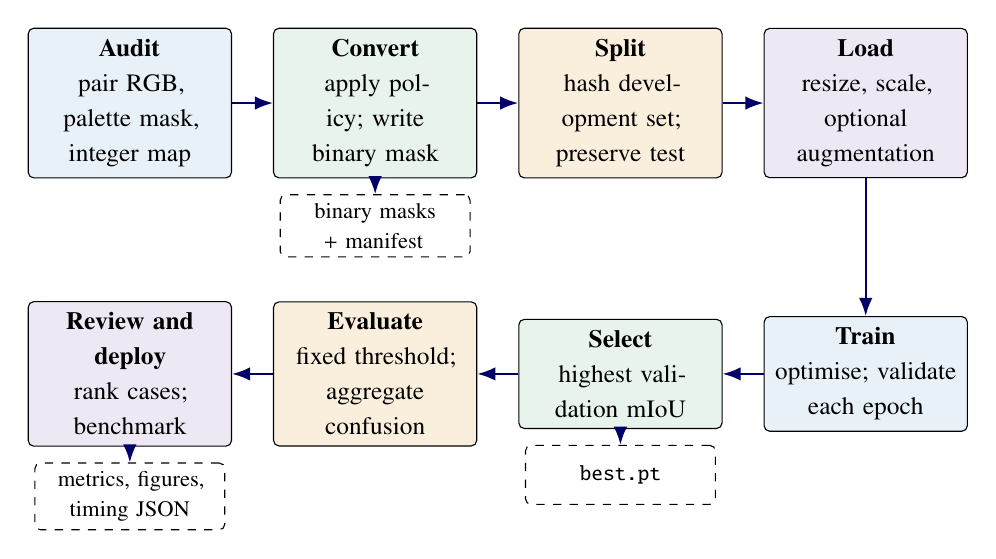
\begin{tikzpicture}[
  node distance=0.52cm,
  pipestep/.style={draw,rounded corners=2pt,text width=2.3cm,minimum height=1.15cm,
    align=center,font=\small,inner sep=4pt},
  artifact/.style={draw,dashed,rounded corners=2pt,text width=2.2cm,minimum height=0.75cm,
    align=center,font=\footnotesize,inner sep=3pt},
  arrow/.style={-{Latex[length=2.3mm]},thick,draw=azulUC3M}
]
\node[pipestep,fill=softblue] (audit) {\textbf{Audit}\\pair RGB, palette mask, integer map};
\node[pipestep,fill=softgreen,right=of audit] (map) {\textbf{Convert}\\apply policy; write binary mask};
\node[pipestep,fill=softorange,right=of map] (split) {\textbf{Split}\\hash development set; preserve test};
\node[pipestep,fill=softpurple,right=of split] (load) {\textbf{Load}\\resize, scale, optional augmentation};
\node[pipestep,fill=softblue,below=1.75cm of load] (train) {\textbf{Train}\\optimise; validate each epoch};
\node[pipestep,fill=softgreen,left=of train] (select) {\textbf{Select}\\highest validation mIoU};
\node[pipestep,fill=softorange,left=of select] (eval) {\textbf{Evaluate}\\fixed threshold; aggregate confusion};
\node[pipestep,fill=softpurple,left=of eval] (review) {\textbf{Review and deploy}\\rank cases; benchmark};
\draw[arrow] (audit) -- (map);
\draw[arrow] (map) -- (split);
\draw[arrow] (split) -- (load);
\draw[arrow] (load) -- (train);
\draw[arrow] (train) -- (select);
\draw[arrow] (select) -- (eval);
\draw[arrow] (eval) -- (review);

\node[artifact,below=0.2cm of map] (manifest) {binary masks + manifest};
\node[artifact,below=0.2cm of select] (checkpoint) {\texttt{best.pt}};
\node[artifact,below=0.2cm of review] (reports) {metrics, figures, timing JSON};
\draw[arrow,dashed] (map) -- (manifest);
\draw[arrow,dashed] (select) -- (checkpoint);
\draw[arrow,dashed] (review) -- (reports);
\end{tikzpicture}
}
\caption[Common implementation workflow.]{Common implementation workflow from
raw CaT files to saved evidence. Dashed boxes are persistent artifacts that
allow a reported result to be traced to its data, selected checkpoint, and
evaluation outputs.}
\label{fig:common_pipeline}
\end{figure}

During training, the data loader shuffles only the training subset. Validation
is deterministic and unaugmented. At the end of each epoch the model is
evaluated on all 266 validation images; \texttt{best.pt} is replaced only if
validation mIoU improves. The checkpoint stores the model state, optimiser
state, epoch, complete configuration, and class weights. The test evaluator
loads that checkpoint, switches the model to evaluation mode, disables
gradients, iterates through the test manifest without shuffling, and
accumulates one $2\times2$ confusion matrix.

The output directory for each experiment contains the training history,
\texttt{best.pt}, \texttt{last.pt}, validation visualisations, test metrics,
and selected review panels. Generated repeat-seed configurations are retained
instead of being assembled only in memory. These decisions make the
experimental procedure inspectable after training hardware is no longer
available.

\section{Annotation Ambiguity and Observable Evidence}
\label{sec:annotation_ambiguity}

For metric computation the CaT mask is ground truth: every disagreement is
counted as model error. For scientific interpretation, however, the annotation
is a human judgement about vehicle capability from a scene. Several cases show
why disagreement cannot always be diagnosed from RGB appearance alone.

In \texttt{mixed\_pln\_1278}, the annotated blue corridor continues through a
pale open area, while the cultivated field at the top of the image is
off-road-only and therefore blocked by the blue+green policy. The field and
track share colour and texture cues in the RGB image. The label may depend on
surface preparation, soil support, crop rows, or the intended route---physical
information that a single frame does not establish.

In \texttt{mixed\_118}, the RGB frame shows dense woodland and a leaf-covered
floor with almost no visually distinct road edge. The annotation nevertheless
assigns a broad, irregular foreground region to the sedan-capable class. Some
of that region may correspond to a faint route visible to the annotator or in
adjacent frames, but its extent is difficult to reconstruct from this image
alone.

\begin{figure}[H]
\centering
\begin{subfigure}[t]{0.485\linewidth}
  \centering
  \includegraphics[width=\linewidth]{../CAT/mixed/Test/imgs/img_pln_1278.png}
  \caption{\texttt{mixed\_pln\_1278}: RGB image.}
\end{subfigure}\hfill
\begin{subfigure}[t]{0.485\linewidth}
  \centering
  \includegraphics[width=\linewidth]{../CAT/mixed/Test/annos/anno_pln_1278.jpg}
  \caption{\texttt{mixed\_pln\_1278}: released annotation.}
\end{subfigure}

\vspace{0.20cm}
\begin{subfigure}[t]{0.485\linewidth}
  \centering
  \includegraphics[width=\linewidth]{../CAT/mixed/Test/imgs/img_118.png}
  \caption{\texttt{mixed\_118}: RGB image.}
\end{subfigure}\hfill
\begin{subfigure}[t]{0.485\linewidth}
  \centering
  \includegraphics[width=\linewidth]{../CAT/mixed/Test/annos/anno_118.jpg}
  \caption{\texttt{mixed\_118}: released annotation.}
\end{subfigure}
\caption[Examples of ambiguity in the available RGB evidence.]{RGB frames and
released CaT annotations for the two cases discussed in the text. In
\texttt{mixed\_pln\_1278}, the pale track and cultivated field have similar
appearance despite different capability labels. In \texttt{mixed\_118}, dense
vegetation and leaf-covered ground provide few clear cues for the broad
accepted foreground region. The annotation colours retain the
original four-class CaT vehicle-capability hierarchy.}
\label{fig:cat_ambiguity_examples}
\end{figure}

Figure~\ref{fig:cat_ambiguity_examples} places the two discussed RGB frames
beside their released annotations so that the ambiguity is visible rather than
asserted only in prose.

In \texttt{mixed\_459}, low vegetation and the track meet along an irregular
foreground edge. Moving the line by several pixels changes the boundary-band
score substantially even though more than one contour may appear plausible
from RGB alone.

These examples do \emph{not} demonstrate that the annotations are wrong. The
annotator may have had route knowledge, higher-resolution context, or a
vehicle-capability convention unavailable in the displayed frame. Conversely,
visual plausibility does not prove physical traversability. CaT provides
neither multiple independent annotations nor inter-annotator agreement, so the
amount of label uncertainty cannot be estimated from the released data. The
thesis can identify cases where RGB evidence is insufficient to justify a
precise boundary, but it cannot calculate a noise rate or replace the supplied
label with a preferred alternative.

This limitation affects both training and evaluation. The model is optimised
to reproduce the annotations, and the reported FSR/FBR describe disagreement
with that policy. They are not direct measurements of real vehicle incidents.
The qualitative chapter therefore distinguishes clear spatial model failures
from cases whose physical status would require additional evidence.

% ============================================================
\chapter{PIDNet-S Model Development}
\label{ch:pidnet}
% ============================================================

\section{Selection Rationale}

The initial goal was to establish a model that could be trained, evaluated,
and plausibly deployed without requiring a high-end GPU. PIDNet-S was selected
because its architecture explicitly separates semantic context, spatial
detail, and boundary information while remaining compact
~\cite{xu2023pidnet}. This matched the main visual structure of CaT: large
connected trail regions require context, small rocks and vegetation edges
require detail, and capability boundaries are safety-relevant.

A conventional encoder--decoder such as U-Net offered a simpler alternative,
whereas a large transformer offered greater representation capacity. Neither
addressed the initial latency constraint as directly. Starting with a
purpose-built real-time network made it possible to develop the complete
pipeline around a compact deployment candidate. The comparative experiments
in Chapter~\ref{ch:rod_extension} subsequently test whether this choice
sacrifices accuracy relative to pretrained encoders and other decoder
families.

The model is trained from scratch. No Cityscapes or ImageNet checkpoint is
loaded. This keeps the baseline self-contained, but it also means later
comparisons with pretrained encoders measure complete model recipes rather
than architecture alone.

\section{Implemented Architecture}

PIDNet's control-system terminology is an analogy. The network does not
calculate a proportional--integral--derivative control command. Its three
branches instead divide the segmentation problem:
\begin{itemize}
  \item the \textbf{P branch} preserves local appearance and spatial
  resolution;
  \item the \textbf{I branch} accumulates semantic context on progressively
  smaller feature grids;
  \item the \textbf{D branch} retains high-frequency differences that help
  locate region boundaries.
\end{itemize}

After a shared stem, the P and D paths remain at one eighth of the input
resolution. The I path reaches one sixteenth, one thirty-second, and one
sixty-fourth resolution. PagFM modules compare P- and I-path features and
selectively inject semantic context into the detail path. Difference features
from the semantic stages update the D branch. PAPPM pools context at multiple
scales at the end of the I path. Light-Bag then uses boundary attention from
the D branch to fuse the spatial and semantic representations
~\cite{xu2023pidnet}.

\begin{figure}[H]
\centering
\resizebox{\textwidth}{!}{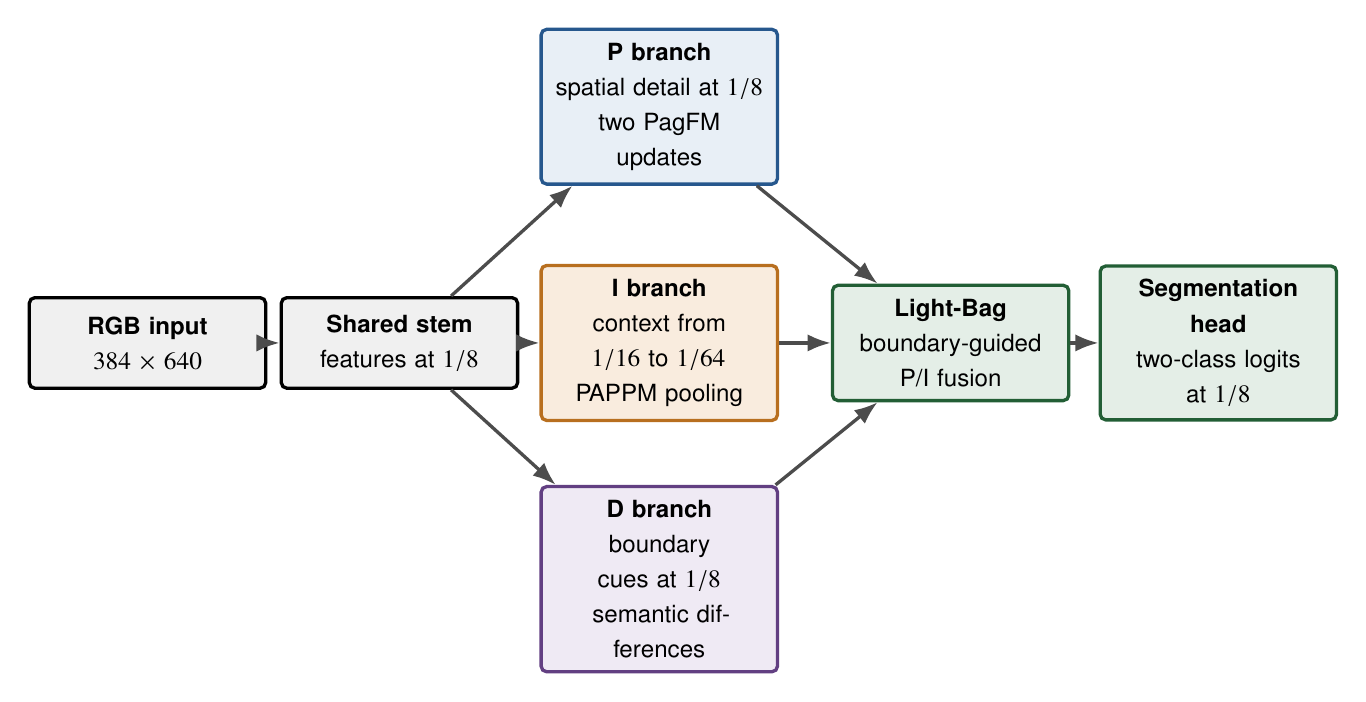
\begin{tikzpicture}[
  font=\sffamily\small,
  >=Latex,
  block/.style={draw, rounded corners=2pt, very thick, align=center,
    minimum height=1.15cm, text width=2.65cm, inner sep=5pt},
  input/.style={block, fill=gray!12},
  pblock/.style={block, draw=pidP!80!black, fill=pidP!11},
  iblock/.style={block, draw=pidI!85!black, fill=pidI!15},
  dblock/.style={block, draw=pidD!80!black, fill=pidD!12},
  fusion/.style={block, draw=pidFuse!75!black, fill=pidFuse!13},
  flow/.style={->, very thick, draw=black!70},
  semantic/.style={->, thick, draw=pidI!85!black},
  detail/.style={->, thick, dashed, draw=pidD!80!black}
]
  \node[input] (rgb) at (0,0) {\textbf{RGB input}\\$384\times640$};
  \node[input] (stem) at (3.2,0) {\textbf{Shared stem}\\features at $1/8$};

  \node[pblock] (p) at (6.5,3.0) {\textbf{P branch}\\spatial detail at $1/8$\\two PagFM updates};
  \node[iblock] (i) at (6.5,0) {\textbf{I branch}\\context from $1/16$ to $1/64$\\PAPPM pooling};
  \node[dblock] (d) at (6.5,-3.0) {\textbf{D branch}\\boundary cues at $1/8$\\semantic differences};

  \node[fusion] (bag) at (10.2,0) {\textbf{Light-Bag}\\boundary-guided\\P/I fusion};
  \node[fusion] (head) at (13.6,0) {\textbf{Segmentation head}\\two-class logits\\at $1/8$};

  \draw[flow] (rgb) -- (stem);
  \draw[flow] (stem) -- (p);
  \draw[flow] (stem) -- (i);
  \draw[flow] (stem) -- (d);

  \draw[flow] (p) -- (bag);
  \draw[flow] (i) -- (bag);
  \draw[flow] (d) -- (bag);
  \draw[flow] (bag) -- (head);
\end{tikzpicture}
}
\caption[Conceptual PIDNet-S three-branch architecture.]{Conceptual PIDNet-S
flow. The P branch retains spatial detail, the I branch extracts context, and
the D branch supplies boundary cues. PagFM, PAPPM, and Light-Bag exchange and
fuse those representations before the segmentation head. Original schematic
drawn for this thesis and adapted from Xu et al.~\cite{xu2023pidnet}.}
\label{fig:final_pidnet_architecture}
\end{figure}

Figure~\ref{fig:final_pidnet_architecture} shows the three processing branches
and the points at which they exchange and fuse features.

The implementation uses the PIDNet-S schedule $(m,n,C)=(2,3,32)$, with 96
pyramid-pooling channels and 128 head channels. $C$ is the base width; $m$ and
$n$ control residual-stage repetition. Table~\ref{tab:pidnet_tensor_shapes}
records the principal shapes for the $640\times384$ input. Listing these
shapes is useful both for implementation verification and for understanding
where computation is spent.

\begin{table}[H]
\centering
\caption{Principal implemented PIDNet-S feature shapes at $640\times384$.}
\label{tab:pidnet_tensor_shapes}
\small
\begin{tabularx}{\textwidth}{@{}lclX@{}}
\toprule
\textbf{Component} & \textbf{Spatial size} & \textbf{Channels} & \textbf{Purpose} \\
\midrule
Shared stem output & $80\times48$ ($1/8$) & 64 & Common input to the three paths \\
P branch & $80\times48$ ($1/8$) & $64\rightarrow128$ & Preserve detail; receive two PagFM updates \\
I stage 3 & $40\times24$ ($1/16$) & 128 & First deeper semantic stage \\
I stage 4 & $20\times12$ ($1/32$) & 256 & Broader contextual representation \\
I stage 5 & $10\times6$ ($1/64$) & 512 & Deepest semantic features before PAPPM \\
PAPPM output & $80\times48$ ($1/8$) & 128 & Multi-scale context returned for fusion \\
D branch & $80\times48$ ($1/8$) & $32\rightarrow64\rightarrow128$ & Boundary-sensitive representation \\
Light-Bag output & $80\times48$ ($1/8$) & 128 & Boundary-guided P/I fusion \\
Binary head & $80\times48$ ($1/8$) & 2 & Native untraversable/traversable logits \\
Wrapper output & $640\times384$ & 2 & Bilinearly upsampled full-resolution logits \\
\bottomrule
\end{tabularx}
\end{table}

Auxiliary P- and D-head outputs are disabled, so the network exposes one final
two-class logits tensor and has 7,623,522 trainable parameters. In the vendored
PIDNet implementation this architectural choice is named
\texttt{augment=False}. It is unrelated to the data-loader
\texttt{augment} flag. Both happen to be false for the retained checkpoint, but
they control different operations.

\begin{figure}[H]
\centering
\resizebox{\textwidth}{!}{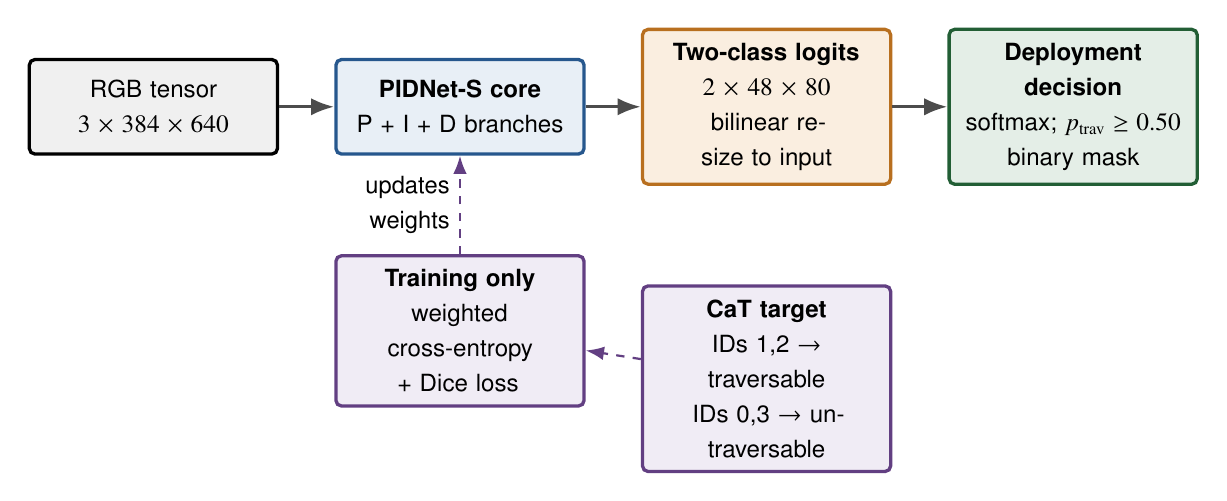
\begin{tikzpicture}[
  font=\sffamily\small,
  >=Latex,
  node distance=0.7cm,
  stage/.style={draw, rounded corners=2pt, very thick, align=center,
    minimum height=1.2cm, text width=2.8cm, inner sep=5pt},
  data/.style={stage, fill=gray!12},
  model/.style={stage, draw=pidP!80!black, fill=pidP!11},
  operation/.style={stage, draw=pidI!85!black, fill=pidI!14},
  output/.style={stage, draw=pidFuse!75!black, fill=pidFuse!13},
  target/.style={stage, draw=pidD!80!black, fill=pidD!11},
  flow/.style={->, very thick, draw=black!70},
  trainflow/.style={->, thick, dashed, draw=pidD!80!black}
]
  \node[data] (rgb) {RGB tensor\\$3\times384\times640$};
  \node[model, right=of rgb] (core) {\textbf{PIDNet-S core}\\P + I + D branches};
  \node[operation, right=of core] (logits) {\textbf{Two-class logits}\\$2\times48\times80$\\bilinear resize to input};
  \node[output, right=of logits] (mask) {\textbf{Deployment decision}\\softmax; $p_{\mathrm{trav}}\geq0.50$\\binary mask};

  \draw[flow] (rgb) -- (core);
  \draw[flow] (core) -- (logits);
  \draw[flow] (logits) -- (mask);

  \node[target, below=1.25cm of logits] (labels) {\textbf{CaT target}\\IDs 1,2 $\rightarrow$ traversable\\IDs 0,3 $\rightarrow$ untraversable};
  \node[target, below=1.25cm of core] (loss) {\textbf{Training only}\\weighted cross-entropy\\+ Dice loss};
  \draw[trainflow] (labels) -- (loss);
  \draw[trainflow] (loss) -- node[left, align=right] {updates\\weights} (core);
\end{tikzpicture}
}
\caption[Implemented PIDNet-S binary pipeline.]{Implemented PIDNet-S binary
pipeline. The one-eighth-resolution logits are returned to the input
resolution before the training loss or deployment decision is calculated.
The lower dashed path is active only during training. Original schematic drawn
for this thesis; the core network follows Xu et al.~\cite{xu2023pidnet}.}
\label{fig:final_pidnet_binary_pipeline}
\end{figure}

Figure~\ref{fig:final_pidnet_binary_pipeline} then connects that core network
to the two-class training and thresholding operations implemented here.

For logits $z_{i0}$ and $z_{i1}$ at pixel $i$, the traversable probability is
\begin{equation}
 p_i =
 \frac{\exp(z_{i1})}
 {\exp(z_{i0})+\exp(z_{i1})}.
 \label{eq:pidnet_softmax}
\end{equation}
Here, $i$ indexes a pixel, $z_{i0}$ and $z_{i1}$ are its untraversable and
traversable logits, $\exp(\cdot)$ is the exponential function, and $p_i$ is
the normalised probability assigned to the traversable class. The other
softmax output, $1-p_i$, is the untraversable probability.
The reference binary prediction is $\hat y_i=\mathbb{1}[p_i\geq0.50]$.
The constant 0.50 is the fixed probability threshold, and equality is assigned
to the traversable class. No morphological cleanup, connected-component filtering, or temporal smoothing
is applied. The output therefore represents the model and threshold directly.

\section{Objective, Optimiser, and Checkpoint Selection}

The main PIDNet objective combines weighted cross-entropy and soft Dice loss.
For classes $c\in\{0,1\}$ and their corresponding weights $w_c$, the
cross-entropy term is
\begin{equation}
 \mathcal{L}_{\mathrm{WCE}}
 =-\frac{1}{N}\sum_{i=1}^{N}w_{y_i}\log p(y_i\mid x).
\end{equation}
In this expression, $\mathcal{L}_{\mathrm{WCE}}$ is weighted cross-entropy,
$N$ is the number of pixels included in the loss, $i$ indexes those pixels,
$y_i\in\{0,1\}$ is the target class, $w_{y_i}$ is the weight of that class,
and $p(y_i\mid x)$ is the probability assigned to the correct class for input
$x$. The natural logarithm is denoted by $\log$.
The implemented Dice term operates on the traversable probability and binary
target. For one image,
\begin{equation}
 \mathcal{L}_{\mathrm{Dice}}
 =1-\frac{2\sum_i p_i y_i+\epsilon}
 {\sum_i p_i+\sum_i y_i+\epsilon},
 \label{eq:pidnet_dice}
\end{equation}
Here, $p_i$ is the traversable probability from
Equation~\ref{eq:pidnet_softmax}, $y_i$ is one for a traversable target and
zero otherwise, each sum covers the pixels of one image, and
$\epsilon=10^{-6}$ prevents division by zero. The resulting
$\mathcal{L}_{\mathrm{Dice}}$ is zero for perfect overlap and approaches one
as overlap is lost. The constant factor 2 is the conventional Dice
normalisation: when prediction and target coincide, the doubled intersection
equals the sum of their two sizes. The batch mean is used. Dice complements per-pixel
cross-entropy with a
region-overlap signal~\cite{milletari2016vnet}. The default total is
\begin{equation}
 \mathcal{L}=\mathcal{L}_{\mathrm{WCE}}+\mathcal{L}_{\mathrm{Dice}}.
\end{equation}
Thus, $\mathcal{L}$ is the scalar objective differentiated during the default
training run, and both component losses enter with unit coefficient.

Class weights are computed from inverse training-pixel frequency. Before
normalisation, the untraversable weight is multiplied by 2.5 and the
traversable weight by 0.75. The two final weights are rescaled to sum to two.
For the fixed split they are $[1.2606075,\,0.7393925]$. The intent was to
discourage false-safe predictions by making errors on the blocked class more
expensive. Because loss weighting changes optimisation rather than directly
optimising FSR, its actual effect must be established experimentally.

An optional false-safe probability penalty was also implemented:
\begin{equation}
 \mathcal{L}_{\mathrm{FS}}
 =\frac{\sum_i p_i\,\mathbb{1}[y_i=0]}
 {\sum_i\mathbb{1}[y_i=0]}.
 \label{eq:false_safe_penalty}
\end{equation}
$i$ indexes the same $N$ loss pixels as above, and both sums run over those
pixels. The indicator $\mathbb{1}[y_i=0]$ selects annotated untraversable pixels, so
the numerator sums their predicted traversable probabilities and the
denominator counts them. Consequently, $\mathcal{L}_{\mathrm{FS}}$ is the
mean traversable probability over the blocked class. With non-negative
coefficient $\lambda_{\mathrm{FS}}$, the tested objective becomes
$\mathcal{L}+\lambda_{\mathrm{FS}}\mathcal{L}_{\mathrm{FS}}$; the ablation uses
$\lambda_{\mathrm{FS}}=0.35$.
This term pushes traversable probability down over all annotated negative
pixels. It was a plausible alternative to class weighting, but the controlled
experiment later showed that the tested coefficient did not improve the
desired rate.

The retained training settings are given in
Table~\ref{tab:frozen_pidnet_training}. AdamW supplies decoupled weight decay
~\cite{loshchilov2019adamw}. Cosine annealing reduces the learning rate from
$2.5\times10^{-4}$ toward $10^{-5}$ over 15 epochs. Bfloat16 automatic mixed
precision is used on CUDA when supported, while model parameters and optimiser
state remain stored in FP32.

\begin{table}[H]
\centering
\caption{Training configuration of the reference PIDNet-S model.}
\label{tab:frozen_pidnet_training}
\small
\begin{tabularx}{\textwidth}{@{}lX@{}}
\toprule
\textbf{Setting} & \textbf{Implemented value and function} \\
\midrule
Initialisation & Random PIDNet-S weights; no pretrained checkpoint \\
Input and batch & $640\times384$ RGB; batch size 4 \\
Epochs & 15 complete passes over 1,002 training images \\
Optimiser & AdamW, initial learning rate $2.5\times10^{-4}$, weight decay $10^{-4}$ \\
Scheduler & Cosine annealing by epoch to minimum learning rate $10^{-5}$ \\
Objective & weighted cross-entropy + traversable soft Dice \\
Class weights & $[1.2606075,\,0.7393925]$ for untraversable/traversable \\
Data augmentation & disabled \\
Mixed precision & bfloat16 autocast on supported CUDA hardware \\
Seed and workers & seed 1337; zero loader worker processes in the portable config \\
Selection & save the epoch with maximum validation mIoU \\
Decision threshold & 0.50, fixed before official test evaluation \\
\bottomrule
\end{tabularx}
\end{table}

After each epoch, all 266 validation images are evaluated without augmentation
or shuffling. A new \texttt{best.pt} is written only if validation mIoU
increases. The retained checkpoint comes from epoch 15, where validation mIoU
is 0.88834. This rule prevents the 544-image test score from participating in
model selection.

\section{Exploratory Development}

The earliest experiments were iterative engineering runs. They are useful
because they show how the system changed, but they are not single-factor
ablations: several settings change together. Table
~\ref{tab:pidnet_iterative_development} lists both configuration and test
outcome so that the later controlled study is not confused with this
exploration.

\begin{table}[H]
\centering
\caption{Exploratory PIDNet-S development runs. Values are test results; the
runs are confounded and do not estimate individual causal effects.}
\label{tab:pidnet_iterative_development}
\footnotesize
\setlength{\tabcolsep}{4pt}
\begin{tabularx}{\textwidth}{@{}p{0.17\textwidth}Xlrrrr@{}}
\toprule
\textbf{Run} & \textbf{Main change(s)} & \textbf{Policy} & \textbf{mIoU} & \textbf{FSR} & \textbf{FBR} & \textbf{Thr.} \\
\midrule
\texttt{default} & Initial pipeline, five epochs & Blue & 0.8374 & 7.24\% & 7.92\% & 0.50 \\
\texttt{conservative} & 15 epochs and biased class weights & Blue & 0.8735 & 3.89\% & 9.67\% & 0.50 \\
\texttt{third\_run} & $720\times448$, false-safe term, 18 epochs & Blue & 0.8219 & 2.32\% & 21.42\% & 0.58 \\
\texttt{fourth\_run} & Remove false-safe term; retain higher resolution & Blue & 0.8544 & 4.08\% & 12.30\% & 0.53 \\
\path{blue_green_best} & Change policy; $640\times384$, 15 epochs & Blue+green & 0.8780 & 4.87\% & 8.34\% & 0.50 \\
\bottomrule
\end{tabularx}
\end{table}

The five-epoch run established that the complete pipeline functioned but left
clear room for learning. Extending training and biasing the loss reduced FSR
while increasing FBR, suggesting a more conservative operating point. The
third run combined higher resolution, an explicit false-safe penalty, and a
0.58 threshold. Its low FSR was accompanied by a very high 21.42\% FBR and
lower mIoU. Because three factors changed, it was impossible to identify the
cause. The fourth run removed the explicit penalty but retained the higher
resolution and a threshold above 0.50; it recovered part of the accuracy but
remained overly conservative.

The blue+green run changed the target vehicle and returned to
$640\times384$. Its result motivated using blue+green as the main operational
policy, but it does not prove that merging green causes an accuracy
improvement: target definition, training history, and class balance differ
from the earlier blue-only runs. This interpretive constraint is retained
throughout the thesis.

The exploratory phase produced two lessons. First, a low FSR can be obtained
by simply blocking more pixels, so FSR must always be read with FBR. Second,
multi-factor iteration can guide engineering but cannot support a claim about
which setting caused the change. Those lessons led to the controlled ablation.

\section{Controlled Configuration Ablation}

The controlled reference uses the blue+green policy, PIDNet-S,
$640\times384$, batch size 4, 15 epochs, seed 1337, augmentation enabled,
biased class weights, CE+Dice, and threshold 0.50. Four variants each change
one factor:
\begin{enumerate}
  \item add the false-safe penalty with weight 0.35;
  \item disable the complete tested augmentation recipe;
  \item increase input to $720\times448$ and reduce batch size to 2 for memory;
  \item replace the computed class weights with neutral $[1,1]$.
\end{enumerate}

The alternatives were chosen to answer practical questions arising from the
exploratory work. The penalty tests whether FSR can be reduced inside the loss
rather than at the threshold. Disabling augmentation tests whether the
synthetic appearance variation matches CaT. Higher resolution tests whether
thin boundaries are limited by input detail. Neutral weights test whether the
manually biased imbalance correction is necessary.

\begin{table}[H]
\centering
\caption{Single-seed controlled PIDNet-S ablation. Bold identifies the
configuration retained for subsequent analysis. Lower FSR and FBR are
preferable.}
\label{tab:pidnet_controlled_ablation}
\small
\begin{tabularx}{\textwidth}{@{}lXrrr@{}}
\toprule
\textbf{Run} & \textbf{One changed factor} & \textbf{mIoU} & \textbf{FSR} & \textbf{FBR} \\
\midrule
Reference & None & 0.8667 & 5.89\% & 8.48\% \\
False-safe loss & Penalty coefficient 0.35 & 0.8177 & 7.45\% & 12.95\% \\
\textbf{Augmentation off} & \textbf{Disable tested flip and photometric recipe} & \textbf{0.8939} & \textbf{4.32\%} & 7.04\% \\
Higher resolution & $720\times448$, batch size 2 & 0.8632 & 5.62\% & 9.28\% \\
Neutral weights & Class weights $[1,1]$ & 0.8848 & 5.28\% & \textbf{6.95\%} \\
\bottomrule
\end{tabularx}
\end{table}

Table~\ref{tab:pidnet_controlled_ablation} supplies the test result for each
one-factor change and marks the retained configuration.

Disabling the tested augmentation improves mIoU by 2.72 percentage points and
reduces both asymmetric error rates relative to the reference. The result
suggests that the colour, blur, and sharpness variations used here do not
represent helpful additional CaT variation. It cannot establish that a
different geometric, weather, or sensor-specific augmentation would also be
harmful.

The false-safe penalty is discarded because it worsens mIoU, FSR, and FBR.
Its gradient pushes traversable probability downward on every negative pixel,
but that global pressure does not guarantee a better thresholded operating
point after optimisation. Higher resolution is also discarded: it increases
pixel computation by 31.25\%, halves the batch size, and does not improve any
headline metric. Neutral weights produce the lowest FBR but a higher FSR and
lower mIoU than augmentation-off. The augmentation-off checkpoint is selected
by validation mIoU. Settings from different rows are not combined after
examining their test results.

Because each row has one seed, the differences provide engineering evidence
rather than estimates of population effects. The separate three-seed
architecture experiment measures repeatability for complete model recipes; it
does not change the statistical scope of this ablation.

\section{Threshold as an Operating Control}

A threshold sweep was conducted on the earlier
\texttt{blue\_green\_best} checkpoint from 0.35 to 0.65. It was not used to
alter the reference checkpoint's 0.50 threshold. Table
~\ref{tab:pidnet_threshold_sweep} shows the expected monotonic trade:
increasing the threshold reduces false-safe openings and increases false
blocks.

\begin{table}[H]
\centering
\caption{Post-hoc threshold sweep on the earlier
\texttt{blue\_green\_best} checkpoint.}
\label{tab:pidnet_threshold_sweep}
\begin{tabular}{@{}rrrr@{}}
\toprule
\textbf{Threshold} & \textbf{mIoU} & \textbf{FSR} & \textbf{FBR} \\
\midrule
0.35 & 0.8774 & 6.14\% & 6.78\% \\
0.40 & 0.8781 & 5.68\% & 7.29\% \\
0.45 & 0.8782 & 5.26\% & 7.81\% \\
0.50 & 0.8780 & 4.87\% & 8.34\% \\
0.55 & 0.8774 & 4.50\% & 8.89\% \\
0.60 & 0.8763 & 4.15\% & 9.49\% \\
0.65 & 0.8747 & 3.80\% & 10.14\% \\
\bottomrule
\end{tabular}
\end{table}

\begin{figure}[H]
\centering
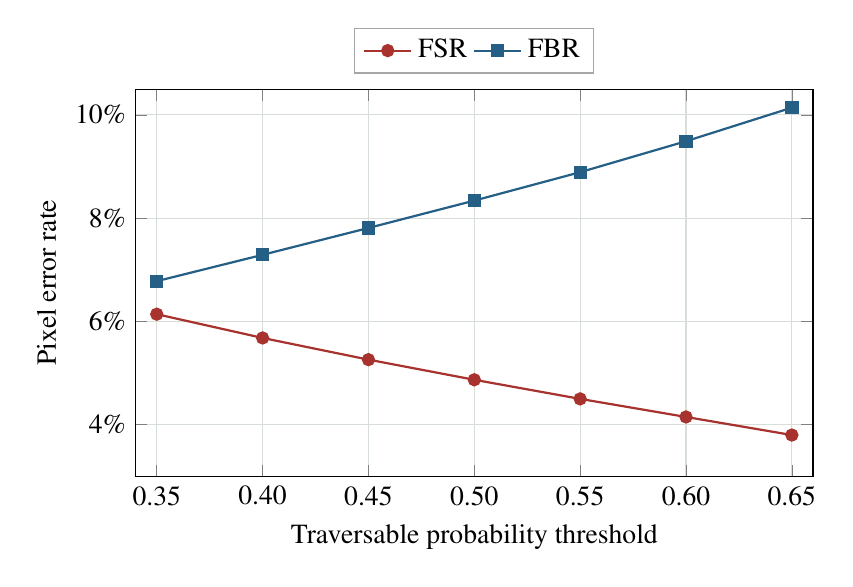
\begin{tikzpicture}
\begin{axis}[
  width=0.84\textwidth,
  height=6.5cm,
  xlabel={Traversable probability threshold},
  ylabel={Pixel error rate},
  ymin=0.03,ymax=0.105,
  xmin=0.34,xmax=0.66,
  xtick={0.35,0.40,0.45,0.50,0.55,0.60,0.65},
  xticklabels={0.35,0.40,0.45,0.50,0.55,0.60,0.65},
  ytick={0.04,0.06,0.08,0.10},
  yticklabels={4\%,6\%,8\%,10\%},
  grid=both,
  grid style={line},
  legend style={
    at={(0.5,1.04)},
    anchor=south,
    legend columns=2,
    fill=white,
    draw=black!35
  }
]
\addplot[color=safety,mark=*,thick] coordinates {
  (0.35,0.0614) (0.40,0.0568) (0.45,0.0526) (0.50,0.0487)
  (0.55,0.0450) (0.60,0.0415) (0.65,0.0380)
};
\addlegendentry{FSR}
\addplot[color=block,mark=square*,thick] coordinates {
  (0.35,0.0678) (0.40,0.0729) (0.45,0.0781) (0.50,0.0834)
  (0.55,0.0889) (0.60,0.0949) (0.65,0.1014)
};
\addlegendentry{FBR}
\end{axis}
\end{tikzpicture}
\caption{False-safe and false-block trade-off under post-hoc threshold
variation. A threshold is an operating choice; it does not improve both error
directions simultaneously.}
\label{fig:pidnet_threshold_plot}
\end{figure}

Figure~\ref{fig:pidnet_threshold_plot} makes the opposing movement of FSR and
FBR across the tested thresholds directly visible.

The maximum observed mIoU occurs at 0.45, but the difference from 0.50 is only
0.0002. More importantly, the sweep uses the test set for characterisation.
Choosing 0.45 from this table and reporting it as an untouched test result
would leak test information into model selection. The final 0.50 operating
point is retained. A deployed threshold should instead be selected on
validation data using an application-defined error cost or risk constraint, then
evaluated once on an independent test set.

\section{Reference Checkpoint}

All subsequent PIDNet-S error analysis, reproduction, CPU, and TensorRT measurements
use the following checkpoint:
\begin{center}
\small\path{outputs/controlled_ablation_augment_off/checkpoints/best.pt}
\end{center}
Keeping the parameters fixed preserves a direct link between the configuration,
manifest, decision threshold, pixel metrics, qualitative panels, and exported
engines. The checkpoint is the strongest PIDNet-S configuration observed in
the controlled study, not an estimate of the architecture's maximum possible
performance. Other augmentation families, pretrained weights, boundary
supervision, longer schedules, or different seed sets could produce a
different result. Its value is that it identifies one model whose behaviour
can be reproduced across evaluation and deployment settings.

% ============================================================
\chapter{ROD and Comparative Architecture Study}
\label{ch:rod_extension}
% ============================================================

\section{Motivation for Pretrained Feature Transfer}

The PIDNet-S analysis exposed a recurring pattern: low-contrast corridors
were sometimes removed, broad fields could be opened incorrectly, and small
boundary displacements survived even in otherwise accurate masks. With only
1,002 training images, one possible remedy is to reuse visual structure learned
from a much larger corpus rather than asking every feature extractor to learn
from CaT alone. ROD provides a concrete instance of this strategy. It connects
a trainable off-road segmentation decoder to a pretrained EfficientSAM ViT-S
encoder whose weights remain fixed during task training
~\cite{sun2025rod,xiong2024efficientsam}.

This design occupies a markedly different operating point from PIDNet-S. It
introduces substantially more representation capacity and transfers pretrained
features, but the full transformer still executes for every frame. Fixed
weights reduce optimisation cost; they do not make inference inexpensive.
Accuracy and latency must therefore be measured together.

The comparison proceeds from controlled pairwise evidence to architectural
context. PIDNet-S and ROD first share the same split, seeds, epoch budget,
objective, and external resolution. Seven additional systems are then trained
under the same protocol. This distinguishes a gain over one reference model
from a gain over the available compact alternatives.

\section{Implemented ROD ViT-S Model}

The ROD implementation contains 29,106,050 parameters. Of these, 22.35 million
belong to the EfficientSAM ViT-S encoder and are frozen; approximately 6.75
million belong to the decoder and are trainable. Freezing is enforced in three
ways: encoder parameters have \texttt{requires\_grad=False}, the encoder is
kept in evaluation mode even when the outer model enters training mode, and
its forward pass is executed under \texttt{no\_grad}. Batch-normalisation in
the decoder remains trainable.

The external input is the same $3\times384\times640$ tensor used by the other
models. Inside ROD it is bilinearly resized to $1024\times1024$ and normalised
with ImageNet statistics. A $16\times16$ patch embedding produces a
$64\times64$ grid of 384-dimensional tokens. The encoder has 12 transformer
blocks with six attention heads. The learned position embedding was pretrained
on a $14\times14$ patch grid and is bicubically interpolated to the $64\times64$
grid.

The released implementation is more specific than the paper's high-level
description. Rather than summing every transformer output, the decoder uses
the outputs of blocks 2 through 12. Each selected feature is
rearranged to channel-first form and projected from 384 to 128 channels by a
$1\times1$ convolution followed by a $3\times3$ convolution. The projected
features are fused sequentially through residual convolutional blocks. A
post-fusion block refines the result and expands it to 256 channels.

Two residual upsampling stages create progressively larger feature maps. The
decoder then resizes four 256-channel sources---the two upsampled maps, the
pre-upsample map, and the encoder's final image embedding---to one common
resolution, concatenates them, and reduces the result to 256 channels. A
$1\times1$ prediction layer produces two logits. They are finally resized to
the original $640\times384$ external input size.

\begin{figure}[H]
\centering
\resizebox{\textwidth}{!}{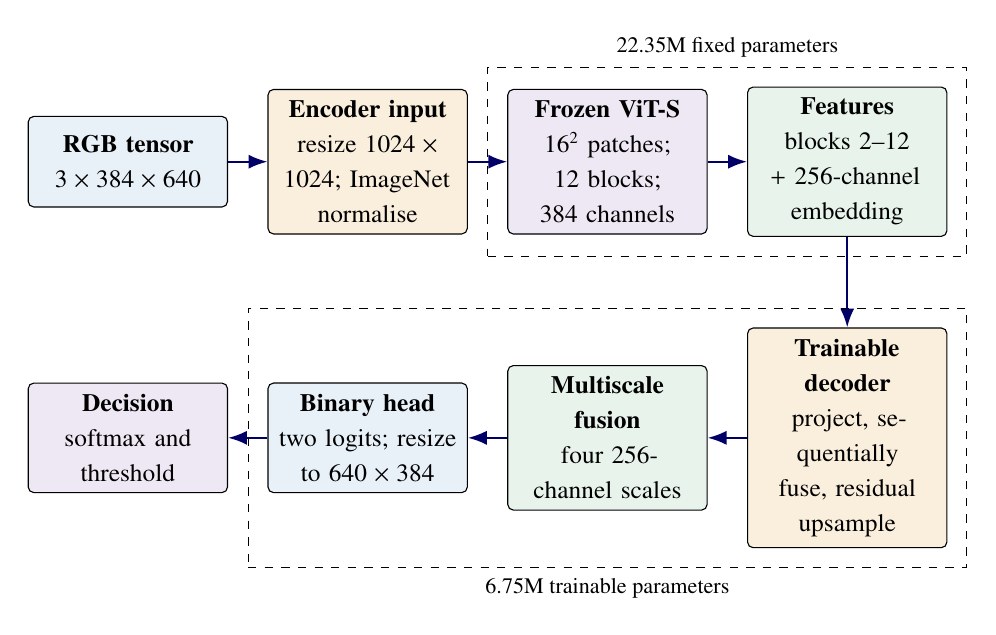
\begin{tikzpicture}[
  node distance=0.5cm,
  block/.style={draw,rounded corners=2pt,minimum height=1.15cm,text width=2.25cm,
    align=center,font=\small,inner sep=4pt},
  arrow/.style={-{Latex[length=2.4mm]},thick,draw=azulUC3M}
]
\node[block,fill=softblue] (rgb) {\textbf{RGB tensor}\\$3\times384\times640$};
\node[block,fill=softorange,right=of rgb] (norm) {\textbf{Encoder input}\\resize $1024\times1024$; ImageNet normalise};
\node[block,fill=softpurple,right=of norm] (vit) {\textbf{Frozen ViT-S}\\$16^2$ patches; 12 blocks; 384 channels};
\node[block,fill=softgreen,right=of vit] (latent) {\textbf{Features}\\blocks 2--12 + 256-channel embedding};
\node[block,fill=softorange,below=1.15cm of latent] (decoder) {\textbf{Trainable decoder}\\project, sequentially fuse, residual upsample};
\node[block,fill=softgreen,left=of decoder] (multi) {\textbf{Multiscale fusion}\\four 256-channel scales};
\node[block,fill=softblue,left=of multi] (head) {\textbf{Binary head}\\two logits; resize to $640\times384$};
\node[block,fill=softpurple,left=of head] (mask) {\textbf{Decision}\\softmax and threshold};
\draw[arrow] (rgb) -- (norm);
\draw[arrow] (norm) -- (vit);
\draw[arrow] (vit) -- (latent);
\draw[arrow] (latent) -- (decoder);
\draw[arrow] (decoder) -- (multi);
\draw[arrow] (multi) -- (head);
\draw[arrow] (head) -- (mask);
\node[draw,dashed,fit=(vit)(latent),inner sep=7pt,label={[font=\footnotesize]above:22.35M fixed parameters}] {};
\node[draw,dashed,fit=(decoder)(multi)(head),inner sep=7pt,label={[font=\footnotesize]below:6.75M trainable parameters}] {};
\end{tikzpicture}
}
\caption[Implemented ROD ViT-S pipeline.]{Implemented ROD ViT-S pipeline. The
pretrained encoder is frozen during CaT training but remains part of every
inference. The decoder uses intermediate blocks 2--12 and multiscale
convolutional fusion before the two-class head.}
\label{fig:rod_architecture}
\end{figure}

Figure~\ref{fig:rod_architecture} distinguishes the frozen feature extractor
from the decoder that is updated on CaT.

Full encoder fine-tuning was an available alternative. It was not adopted
because ROD's defining transfer strategy holds the encoder fixed, the CaT
training set is small, and fine-tuning would greatly increase training memory
and the number of task-specific degrees of freedom. The experiment consequently
does not determine whether end-to-end EfficientSAM adaptation would improve the
result.

\section{Controlled PIDNet--ROD Comparison}

The matched comparison uses seeds 1337, 2027, and 4242 under both blue-only and
blue+green label policies. Within a policy, PIDNet-S and ROD receive:
\begin{itemize}
  \item the same 1,002/266/544 manifest assignment;
  \item the same $640\times384$ external tensors and batch size 4;
  \item 15 epochs and validation-mIoU checkpoint selection;
  \item AdamW at $2.5\times10^{-4}$ with weight decay $10^{-4}$;
  \item epoch-level cosine annealing to $10^{-5}$;
  \item the same deterministic augmentation recipe;
  \item biased inverse-frequency class weights, CE+Dice, and threshold 0.50.
\end{itemize}

Matching these decisions prevents a favourable ROD optimiser, seed, or split
from explaining the comparison. It does not make the two networks identical
experiments in every respect: ROD uses pretrained frozen encoder weights,
model-specific normalisation, and an internal $1024\times1024$ transformer input,
whereas PIDNet-S is randomly initialised and operates directly on the external
resolution. The result therefore compares the complete model pipelines under
common task-level controls.

Population mean and population standard deviation are reported:
\begin{align}
 \bar m &= \frac{1}{3}\sum_{k=1}^{3}m_k,\\
 \sigma_{\mathrm{pop}}
 &=\sqrt{\frac{1}{3}\sum_{k=1}^{3}(m_k-\bar m)^2}.
\end{align}
Here, $m_k$ is the value of the reported metric in run $k$; the index
$k\in\{1,2,3\}$ corresponds to seeds 1337, 2027, and 4242; $\bar m$ is their
arithmetic mean; and $\sigma_{\mathrm{pop}}$ is their population standard
deviation. The divisor is three because the equations describe the complete
declared set of runs rather than estimating variance from a random sample.
With only three selected seeds, the standard deviation describes observed
repeatability; it is not a confidence interval over all possible training
runs.

\section{Reconstructed ROD Training Regime}

The controlled recipe answers a fair architecture-comparison question, but it
does not use the optimisation choices documented for ROD. A second experiment
therefore transfers the published settings as closely as the available
description permits. Table~\ref{tab:rod_recipe_config} contrasts the two
recipes.

\begin{table}[H]
\centering
\caption{Training choices held in the controlled architecture comparison and
their counterparts in the closest documented ROD recipe.}
\label{tab:rod_recipe_config}
\small
\begin{tabularx}{\textwidth}{@{}lXX@{}}
\toprule
\textbf{Setting} & \textbf{Controlled comparison} & \textbf{ROD paper approximation} \\
\midrule
Objective & weighted cross-entropy + Dice & cross-entropy only \\
Class weights & inverse frequency with 2.5/0.75 biases & neutral $[1,1]$ \\
AdamW learning rate & $2.5\times10^{-4}$ & $10^{-3}$ \\
Weight decay & $10^{-4}$ & 0.01 \\
Batch size & 4 & 8 (validation 4) \\
Schedule & epoch-level cosine to $10^{-5}$ & iteration-level polynomial, power 0.9 \\
Augmentation & common tested recipe enabled & disabled because none is documented \\
Epoch budget & 15 & 15 retained because publication does not specify one \\
Threshold & 0.50 & 0.50 \\
\bottomrule
\end{tabularx}
\end{table}

The polynomial scheduler updates after every optimiser step:
\begin{equation}
 \eta_t=\eta_0\left(1-\frac{t}{T}\right)^{0.9},
\end{equation}
where $\eta_t$ is the learning rate after optimiser step $t$, $\eta_0=10^{-3}$
is the initial learning rate, $T$ is the total number of optimiser steps in
15 epochs, and $0.9$ is the fixed polynomial-decay exponent transferred from
the documented recipe. The step index runs from $t=0$ to $t=T$. The run uses
bfloat16 mixed precision, the official EfficientSAM ViT-S checkpoint, and a
frozen encoder. Because the ROD paper does not disclose its epoch budget,
augmentation policy, or all timing details, this experiment is called the
\emph{closest documented recipe}. It is evidence about transfer of the
reported settings to CaT, not an exact reproduction of a published CaT result.

\section{Architecture Set}

After the PIDNet--ROD comparison, seven additional compact systems were added:
FPN/MobileNetV2, FPN/EfficientNet-B0, U-Net/MobileNetV2,
U-Net/EfficientNet-B0, SegFormer-B0, DDRNet-23-Slim, and BiSeNetV2. With
PIDNet-S and ROD this yields nine model systems. Each is trained for the same
three seeds under both label policies, producing 54 scored runs.

FPN and U-Net are paired with both encoders to separate, within this limited
factorial subset, encoder and decoder effects. MobileNetV2 provides the lighter
convolutional encoder; EfficientNet-B0 provides a somewhat higher-capacity
compact encoder. SegFormer-B0 supplies a hierarchical transformer comparison.
DDRNet-23-Slim and BiSeNetV2 represent architectures designed specifically for
real-time segmentation.

Table~\ref{tab:model_implementation_details} records exact parameter counts
and initialisation. FPN, U-Net, and SegFormer are created through
\texttt{segmentation-models-pytorch}. DDRNet-23-Slim and BiSeNetV2 are adapted
from released PyTorch implementations under their licences. Every wrapper
returns one full-resolution two-class logits tensor so that the common loss and
metrics see the same interface.

\begin{table}[H]
\centering
\caption{Exact model systems, parameter counts, and initialisation in the
comparative study.}
\label{tab:model_implementation_details}
\small
\begin{tabularx}{\textwidth}{@{}lrlX@{}}
\toprule
\textbf{System} & \textbf{Parameters} & \textbf{Initialisation} & \textbf{Implementation note} \\
\midrule
PIDNet-S & 7,623,522 & Random & One final head; PAPPM and Light-Bag \\
ROD ViT-S & 29,106,050 & EfficientSAM ViT-S & 22.35M encoder parameters frozen \\
FPN/MobileNetV2 & 4,215,554 & ImageNet encoder & SMP FPN with \texttt{mobilenet\_v2} \\
FPN/EfficientNet-B0 & 5,759,614 & ImageNet encoder & SMP FPN with \texttt{efficientnet-b0} \\
U-Net/MobileNetV2 & 6,629,090 & ImageNet encoder & SMP U-Net with \texttt{mobilenet\_v2} \\
U-Net/EfficientNet-B0 & 6,251,614 & ImageNet encoder & SMP U-Net with \texttt{efficientnet-b0} \\
SegFormer-B0 & 3,714,658 & ImageNet MiT-B0 & SMP SegFormer decoder \\
DDRNet-23-Slim & 5,694,882 & Random & Two-resolution network; no stable pretrained checkpoint used \\
BiSeNetV2 & 3,341,202 & Released pretrained backbone & Auxiliary heads disabled for the common loss \\
\bottomrule
\end{tabularx}
\end{table}

Initialisation is not hidden because it is a major experimental factor on a
small dataset. PIDNet-S and DDRNet start from random weights; the other seven
systems use some form of pretraining, although ROD freezes its pretrained
encoder while the standard ImageNet encoders are trainable. The benchmark
therefore ranks the implemented recipes. It cannot isolate the causal effect
of architecture from pretraining without additional within-family
pretrained-versus-random experiments.

\section{Fixed-Budget Experimental Scope}

For every comparative run, the external input is $640\times384$, the
batch size is 4, the epoch budget is 15, and the model is selected by validation
mIoU. AdamW, the learning rate, cosine schedule, common CE+Dice objective,
policy-specific class weights, augmentation, 0.50 threshold, and three seeds
are fixed. Blue-only and blue+green experiments write to distinct processed
roots and output directories so that one policy cannot overwrite the other.

These controls support a restricted statement: under the tested CaT recipe,
model A has a higher three-seed mean than model B. They do not prove that the
ranking would remain under model-specific hyperparameter tuning, longer
training, more seeds, another dataset, or an embedded runtime. In particular,
the common 15-epoch budget may favour pretrained systems that converge quickly
and disadvantage randomly initialised models.

The nine-system experiment places the pairwise result in context. ROD's
advantage over PIDNet-S remains clear, but several pretrained
encoder--decoder systems achieve higher CaT overlap under the common recipe.
The results are therefore interpreted as a ranking of complete training
systems, with small differences read against their observed between-seed
variation.

\section{Convergence-Aware Blue+Green Follow-Up}

The 15-epoch matrix answers a matched-compute question, but the saved
validation histories show that it stops while several models are still
improving. A second experiment therefore repeats all nine architectures and
three seeds for the principal blue+green policy. It retains the same data,
external resolution, augmentation, objective, class weighting, optimiser,
initial learning rate, weight decay, threshold, and seed identities. Only the
training horizon and stopping rule change.

The follow-up sets 300 epochs as a ceiling, not as a presumed optimum. Cosine
decay runs from $2.5\times10^{-4}$ to $10^{-5}$ over the first 60 epochs; the
learning rate then remains at $10^{-5}$. Training cannot stop before epoch 60.
After that point it stops when validation mIoU has failed to improve by an
absolute increase of at least $10^{-4}$ on the 0-to-1 mIoU scale for 25
epochs. The checkpoint writer remains slightly more
sensitive than the stopping counter: it stores any strict validation-mIoU
increase, even if the increase is smaller than $10^{-4}$. Consequently, a
run may save its numerically highest checkpoint near the stopping epoch
without resetting the early-stopping counter.

This design gives every run time to pass the early learning phase while still
bounding unnecessary work after the validation curve has flattened. The
selected epoch is therefore called the \emph{validation-selected checkpoint
epoch}; it is not described as the universally optimal epoch for that
architecture. Model-specific objectives and schedules could still change both
the selected epoch and the final ranking.

% ============================================================
\chapter{Experimental Protocols and Evaluation Methods}
\label{ch:protocols}
% ============================================================

\section{Experimental Phases}

The complete experimental campaign is separated into seven phases so that an
exploratory observation is not mistaken for controlled evidence.

\begin{figure}[H]
\centering
\resizebox{\textwidth}{!}{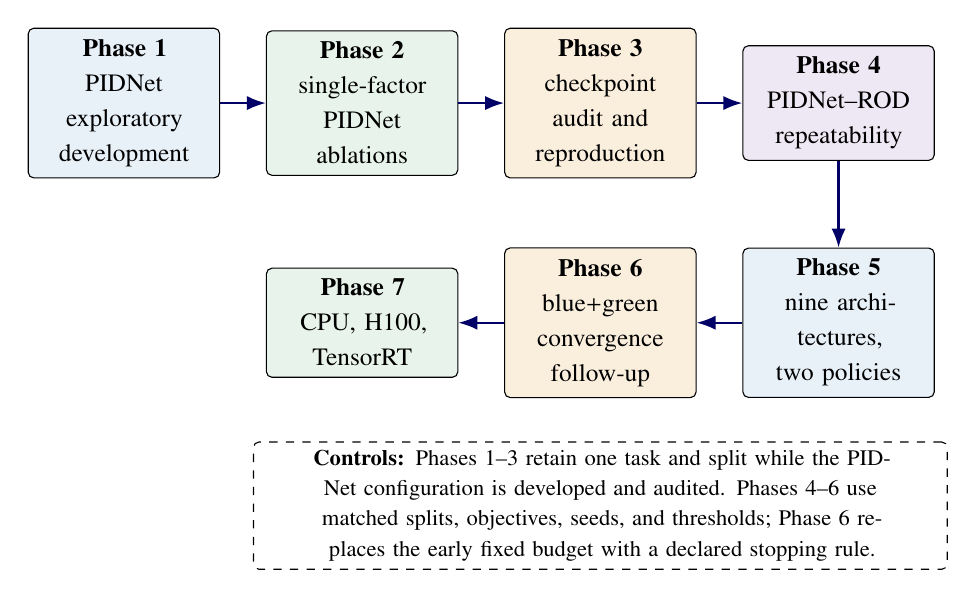
\begin{tikzpicture}[
  node distance=0.58cm,
  phase/.style={draw,rounded corners=2pt,text width=2.15cm,minimum height=1.2cm,
    align=center,font=\small,inner sep=4pt},
  control/.style={draw,dashed,rounded corners=2pt,text width=8.6cm,minimum height=0.8cm,
    align=center,font=\footnotesize,inner sep=3pt},
  arrow/.style={-{Latex[length=2.4mm]},thick,draw=azulUC3M}
]
\node[phase,fill=softblue] (explore) {\textbf{Phase 1}\\PIDNet exploratory development};
\node[phase,fill=softgreen,right=of explore] (ablate) {\textbf{Phase 2}\\single-factor PIDNet ablations};
\node[phase,fill=softorange,right=of ablate] (freeze) {\textbf{Phase 3}\\checkpoint audit and reproduction};
\node[phase,fill=softpurple,right=of freeze] (rod) {\textbf{Phase 4}\\PIDNet--ROD repeatability};
\node[phase,fill=softblue,below=1.1cm of rod] (wide) {\textbf{Phase 5}\\nine architectures, two policies};
\node[phase,fill=softorange,left=of wide] (converge) {\textbf{Phase 6}\\blue+green convergence follow-up};
\node[phase,fill=softgreen,left=of converge] (deploy) {\textbf{Phase 7}\\CPU, H100, TensorRT};
\draw[arrow] (explore) -- (ablate);
\draw[arrow] (ablate) -- (freeze);
\draw[arrow] (freeze) -- (rod);
\draw[arrow] (rod) -- (wide);
\draw[arrow] (wide) -- (converge);
\draw[arrow] (converge) -- (deploy);
\node[control,below=0.55cm of converge] {
  \textbf{Controls:} Phases 1--3 retain one task and split while the PIDNet
  configuration is developed and audited. Phases 4--6 use matched splits,
  objectives, seeds, and thresholds; Phase 6 replaces the early fixed budget
  with a declared stopping rule.
};
\end{tikzpicture}
}
\caption[Experimental phases and controls.]{Experimental phases and their
principal controls. Dataset identity, target policy, and metric definitions
remain fixed as the question changes from configuration selection to model
comparison and runtime measurement.}
\label{fig:experimental_design}
\end{figure}

Figure~\ref{fig:experimental_design} provides the overview; the paragraphs
below state the purpose and controls of each phase.

\textbf{Phase 1: exploratory PIDNet development.} Five runs changed multiple
settings to obtain a working pipeline and reveal promising or problematic
directions. These runs guide questions; they do not isolate causal factors.

\textbf{Phase 2: controlled PIDNet ablation.} A reference configuration and
four one-factor variants test augmentation, false-safe penalty, resolution,
and class weights. All other recorded settings are held fixed. One seed is
used, so this is a controlled engineering comparison without a variance
estimate.

\textbf{Phase 3: checkpoint audit.} The validation-selected augmentation-off
PIDNet checkpoint is identified, reevaluated, qualitatively ranked, and
benchmarked. Subsequent measurements refer to these saved parameters.

\textbf{Phase 4: PIDNet--ROD repeatability.} Both architectures are
trained for seeds 1337, 2027, and 4242 under blue-only and blue+green policies
with one controlled recipe. Separate ROD runs use the optimisation settings
that can be reconstructed from the publication.

\textbf{Phase 5: architecture matrix.} Seven additional systems complete a
nine-model, three-seed, two-policy matrix. Every policy contains 27 scored
model--seed records; together the two ledgers contain 54.

\textbf{Phase 6: convergence-aware follow-up.} The nine-model, three-seed
matrix is repeated for the principal blue+green policy with a 300-epoch
ceiling, 60-epoch cosine decay, a 60-epoch minimum, and validation-based early
stopping. This phase contains another 27 scored model--seed records.

\textbf{Phase 7: runtime evaluation.} Models are timed on a Ryzen~5~5500 CPU
and a common H100 MIG server protocol. The reference PIDNet checkpoint and the
reconstructed ROD checkpoint are also exported to TensorRT and evaluated on an
RTX~5060.

All experiments exclude the official CaT test images from gradient updates and
automatic checkpoint selection. The test set is nevertheless evaluated for
multiple exploratory, ablation, and architecture runs over the lifetime of the
project. It should therefore be understood as a consistently held-out
benchmark partition, not as a single-use blinded set whose scores were hidden
until every engineering decision was complete. Model checkpoints are selected
by validation mIoU, but repeated human inspection of test reports remains a
possible source of research-level selection bias.

\section{Training Procedure}

Each scored run follows the same operational sequence:
\begin{enumerate}
  \item load one complete YAML configuration and set the Python, NumPy, and
  PyTorch random seeds;
  \item construct training and validation datasets from the processed
  manifest, enabling augmentation only for training when configured;
  \item compute class weights from training masks only, or load explicit
  neutral weights;
  \item build the named two-class model and AdamW optimiser;
  \item for every epoch, shuffle the training loader, compute the configured
  loss, backpropagate, update weights, and advance the scheduler;
  \item run an unaugmented validation pass, accumulating its confusion matrix;
  \item write the epoch history and \texttt{last.pt}; replace
  \texttt{best.pt} if validation mIoU exceeds the previous maximum;
  \item after training, load \texttt{best.pt} in the evaluator and score the
  complete test split without gradients or shuffling.
\end{enumerate}

Non-finite training loss or validation metrics raise an error rather than
silently saving a checkpoint. Mixed precision uses bfloat16 when CUDA supports
it and falls back to float16 otherwise. The ordinary 15-epoch experiments do
not use early stopping; every model receives the same maximum number of
training passes. This fixed budget improves protocol matching but is not
necessarily optimal for every architecture.

The convergence-aware blue+green follow-up uses the same operational sequence
with three changes. The epoch ceiling is 300, cosine decay reaches the minimum
learning rate at epoch 60 and then holds it constant, and early stopping is
enabled only after epoch 60. The stopping counter requires an improvement of
at least $10^{-4}$ in validation mIoU and has patience 25. Checkpoint saving
uses any strict improvement, so it can record a slightly higher value that is
too small to reset the patience counter. Every reported test result still
comes from \texttt{best.pt}, never from the final in-memory epoch.

The test evaluator computes weighted cross-entropy loss using the class weights
stored in the checkpoint. Quality metrics are derived independently from
thresholded predictions, so the test loss and mIoU need not rank models in the
same order. The prediction interface is normalised to one full-resolution
two-logit tensor even for third-party architectures that can expose auxiliary
outputs.

\section{Confusion Matrix Convention}

Traversable is always the positive class. The aggregated confusion matrix is
\begin{equation}
\mathbf{C}=
\begin{bmatrix}
 \mathrm{TN} & \mathrm{FP}\\
 \mathrm{FN} & \mathrm{TP}
\end{bmatrix},
\label{eq:confusion_convention}
\end{equation}
Here, $\mathbf{C}$ is the test-wide count matrix; TN, FP, FN, and TP denote
true-negative, false-positive, false-negative, and true-positive pixel counts.
Rows are ground truth and columns are prediction. This ordering is
published because false-safe and false-block terminology can otherwise obscure
which denominator is used.

Figure~\ref{fig:confusion_matrix_visual} reads the same matrix as two
operational questions. The upper ground-truth row contains all pixels that
should be blocked and supplies the denominator of FSR. The lower row contains
all pixels that should be traversable and supplies the denominator of FBR.

\begin{figure}[H]
\centering
\resizebox{\textwidth}{!}{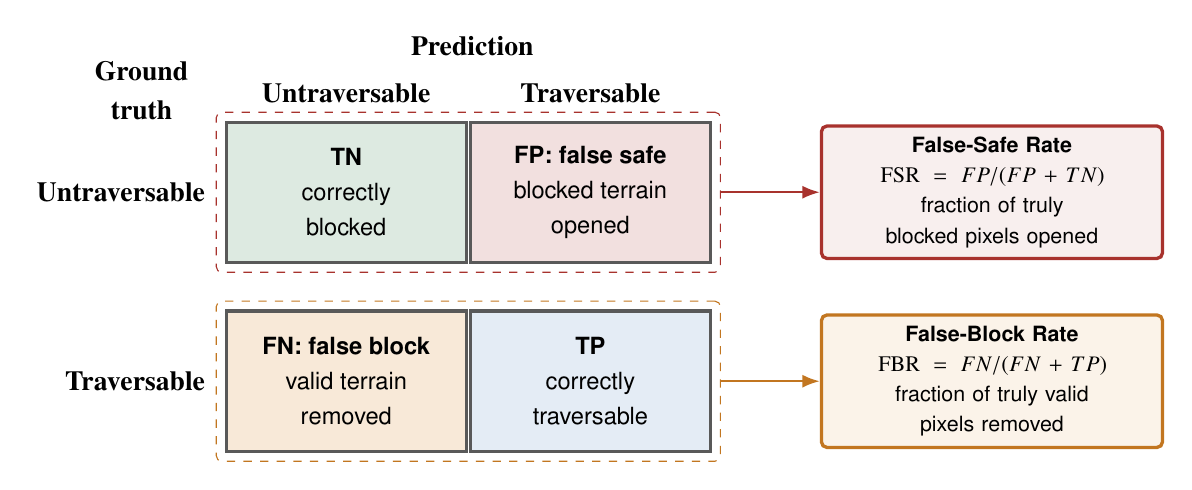
\begin{tikzpicture}[
  font=\sffamily\small,
  cell/.style={draw=black!65,very thick,minimum width=3.05cm,
    minimum height=1.78cm,align=center,inner sep=5pt},
  metric/.style={draw,rounded corners=2pt,very thick,align=center,
    text width=4.05cm,minimum height=1.62cm,inner sep=4pt,
    font=\sffamily\footnotesize},
  link/.style={-{Latex[length=2.2mm]},thick}
]
  \node[font=\bfseries] at (5.05,4.90) {Prediction};
  \node[font=\bfseries,align=center] at (0.85,4.34) {Ground\\truth};
  \node[font=\bfseries] at (3.45,4.30) {Untraversable};
  \node[font=\bfseries] at (6.55,4.30) {Traversable};
  \node[font=\bfseries,anchor=east] at (1.78,3.05) {Untraversable};
  \node[font=\bfseries,anchor=east] at (1.78,0.65) {Traversable};

  \node[cell,fill=good!16] (tn) at (3.45,3.05)
    {\textbf{TN}\\correctly\\blocked};
  \node[cell,fill=safety!15] (fp) at (6.55,3.05)
    {\textbf{FP: false safe}\\blocked terrain\\opened};
  \node[cell,fill=warn!18] (fn) at (3.45,0.65)
    {\textbf{FN: false block}\\valid terrain\\removed};
  \node[cell,fill=pidP!13] (tp) at (6.55,0.65)
    {\textbf{TP}\\correctly\\traversable};

  \node[draw=safety,dashed,rounded corners=2pt,fit=(tn)(fp),inner sep=3pt] (rowu) {};
  \node[draw=warn!90!black,dashed,rounded corners=2pt,fit=(fn)(tp),inner sep=3pt] (rowt) {};
  \node[metric,draw=safety,fill=safety!8] (fsr) at (11.65,3.05)
    {\textbf{False-Safe Rate}\\$\FSR=FP/(FP+TN)$\\
    fraction of truly blocked pixels opened};
  \node[metric,draw=warn!90!black,fill=warn!10] (fbr) at (11.65,0.65)
    {\textbf{False-Block Rate}\\$\FBR=FN/(FN+TP)$\\
    fraction of truly valid pixels removed};
  \draw[link,draw=safety] (rowu.east) -- (fsr.west);
  \draw[link,draw=warn!90!black] (rowt.east) -- (fbr.west);
\end{tikzpicture}
}
\caption[Visual interpretation of the binary confusion matrix.]{Visual
interpretation of the binary confusion matrix and the two asymmetric error
rates. A false safe opens annotated blocked terrain; a false block removes
annotated traversable terrain. Original schematic drawn for this thesis.}
\label{fig:confusion_matrix_visual}
\end{figure}

\begin{table}[H]
\centering
\caption{Operational interpretation of the four binary outcomes.}
\label{tab:confusion_interpretation}
\small
\begin{tabularx}{\textwidth}{@{}lllX@{}}
\toprule
\textbf{Ground truth} & \textbf{Prediction} & \textbf{Count} & \textbf{Interpretation} \\
\midrule
Untraversable & Untraversable & TN & Correctly preserves a blocked pixel \\
Untraversable & Traversable & FP & False safe: opens a pixel outside the annotated capability envelope \\
Traversable & Untraversable & FN & False block: removes an annotated feasible pixel \\
Traversable & Traversable & TP & Correctly preserves a feasible pixel \\
\bottomrule
\end{tabularx}
\end{table}

Table~\ref{tab:confusion_interpretation} states the corresponding operational
meaning of each matrix entry.

All principal test metrics use one matrix accumulated over every pixel in the
split. They are therefore micro-aggregated by pixel. An image with more pixels
would contribute more decisions, although fixed evaluation resizing makes all
544 test images equal in pixel count. Per-image metrics are used only for
qualitative ranking.

\section{Accuracy and Asymmetric Error Metrics}

For class $c$, Intersection over Union is
\begin{equation}
 \operatorname{IoU}_c=
 \frac{\operatorname{TP}_c}
 {\operatorname{TP}_c+\operatorname{FP}_c+\operatorname{FN}_c}.
\end{equation}
Here, $c$ denotes one semantic class, and $\operatorname{TP}_c$,
$\operatorname{FP}_c$, and $\operatorname{FN}_c$ count pixels treated as true
positives, false positives, and false negatives when $c$ is considered the
positive class. The operator $\operatorname{IoU}_c$ is therefore the
intersection of prediction and target for $c$ divided by their union.
For the binary convention this becomes
\begin{align}
 \operatorname{IoU}_{\mathrm{trav}}
 &=\frac{\mathrm{TP}}{\mathrm{TP}+\mathrm{FP}+\mathrm{FN}},\\
 \operatorname{IoU}_{\mathrm{untrav}}
 &=\frac{\mathrm{TN}}{\mathrm{TN}+\mathrm{FP}+\mathrm{FN}},\\
 \operatorname{mIoU}
 &=\frac{\operatorname{IoU}_{\mathrm{trav}}
 +\operatorname{IoU}_{\mathrm{untrav}}}{2}.
\end{align}
The subscripts $\mathrm{trav}$ and $\mathrm{untrav}$ denote traversable and
untraversable. In the latter equation, TN becomes the intersection because the
negative class in the global convention is treated as the class of interest.
The unweighted mean prevents the more frequent class from completely
determining the headline score.

Traversable precision, recall, and F1 are
\begin{align}
 P&=\frac{\mathrm{TP}}{\mathrm{TP}+\mathrm{FP}},&
 R&=\frac{\mathrm{TP}}{\mathrm{TP}+\mathrm{FN}},&
 F1&=\frac{2PR}{P+R}.
\end{align}
Here, $P$ is traversable precision, $R$ is traversable recall, and $F1$ is
their harmonic mean. F1 describes positive-class overlap through precision
and recall but does not
describe true-negative performance. It is therefore reported beside rather
than instead of mIoU.

The two safety-oriented rates are
\begin{align}
 \FSR&=\frac{\mathrm{FP}}{\mathrm{FP}+\mathrm{TN}},
 \label{eq:final_fsr}\\
 \FBR&=\frac{\mathrm{FN}}{\mathrm{FN}+\mathrm{TP}}.
\label{eq:final_fbr}
\end{align}
In these equations, $\FSR$ is False-Safe Rate and $\FBR$ is False-Block Rate;
the four count symbols retain the definitions in
Table~\ref{tab:confusion_interpretation}. FSR conditions on truly
untraversable pixels and asks what fraction the model
opens. FBR conditions on truly traversable pixels and asks what fraction the
model blocks. FBR is equal to one minus traversable recall; it is retained as
a named metric because its operational meaning is clearer in this task.

The two errors matter differently. A connected false-safe area can allow a
planner to consider terrain outside the vehicle's annotated capability, while
a false block can make a feasible route disappear or cause a conservative
stop. Reducing one by moving the threshold usually increases the other. A
useful system must therefore report both. Neither rate includes distance from
the vehicle, trajectory intersection, connected-component size, severity of
terrain, prediction confidence, or actual vehicle outcomes. They are
safety-oriented diagnostic metrics, not safety probabilities.

\section{Multi-Seed Reporting}

For the nine-model comparison, the metric for each model and policy is reported as
mean $\pm$ population standard deviation over three fixed seeds. Population
standard deviation is used because the purpose is to describe those three
executed runs, not to estimate an unknown variance from a random sample.

The seed set controls random initialisation, loader order, and deterministic
augmentation sequences. It does not capture dataset-split uncertainty because
all seeds use the same manifest assignment. It also does not capture
hyperparameter uncertainty. A difference smaller than the observed run-to-run
standard deviation is treated cautiously. In the 15-epoch blue+green matrix,
the top FPN/EfficientNet-B0 and U-Net/EfficientNet-B0 means differ by only
0.02 percentage points. In the convergence-aware follow-up,
FPN/EfficientNet-B0 is higher in all three executed seeds and its mean lead is
0.13 points. This is a consistent observed ordering for the declared suite,
but three selected seeds still do not establish universal superiority or
provide a confidence interval. The matched pairwise comparison shows the same
complete consistency: ROD records higher test mIoU than PIDNet-S in all six of
its policy--seed runs.

\section{Qualitative Review Protocol}

Aggregate metrics reveal how many pixels are wrong but not how those errors
are arranged. The reference PIDNet checkpoint is therefore applied to all 544
test images and each image is assigned:
\begin{itemize}
  \item per-image FSR;
  \item per-image FBR;
  \item combined error $\FSR+\FBR$ for distributional ranking;
  \item boundary-band error.
\end{itemize}

The ground-truth boundary band is formed from the morphological difference
between a two-pixel dilation and a two-pixel erosion. Boundary error is the
fraction of pixels inside that band whose predicted class differs from the
target. The band emphasises local contour placement but can be unstable for
very thin regions and visually ambiguous annotations; it is a diagnostic, not
an alternative headline metric.

The representative-range panel uses mechanically selected images near the
10th, 30th, 50th, 70th, and 90th percentiles of combined per-image error.
Separate ranked panels select the maximum FSR, maximum FBR, and a severe
boundary error. This procedure avoids selecting only visually attractive
successes. The captions report identifiers and rates so the relationship
between the visible mask and the numerical metric can be checked.

The checkpoint is also applied to 130 frames from the external, unlabelled
ALICE mobile-robot sequences (scenario~02, sequences~01--05). Four frames are
displayed to span several path and illumination conditions. ALICE is not used
for training, and no ground-truth masks are available in this study. The panel
can show whether predictions are connected, responsive to scene change, or
visibly implausible; it cannot measure accuracy, FSR, FBR, calibration, or
domain generalisation.

\section{CPU and H100 Timing Protocols}

The CPU platform is an AMD Ryzen~5~5500 with six cores and twelve hardware
threads. PyTorch uses six inference threads, batch size 1, and
$640\times384$ input. Thirty-two test tensors are preloaded. Two complete
warm-up rounds are excluded, followed by five measured repeats, for 160 timed
inferences. Eager execution and \texttt{torch.compile} execution are measured
for all nine comparison models. Compilation occurs during warm-up and is
excluded from the timed samples.

The CPU timer covers model forward, full-resolution logits, softmax, and
thresholded prediction. It excludes image decoding, camera acquisition,
visualisation, and disk output. The reference PIDNet and ROD results are tied
to PyTorch 2.13.0, Python 3.12.12, and their exact checkpoints. ROD retains the
common $640\times384$ external input but resizes it internally to
$1024\times1024$ before its transformer encoder.

The common server measurement uses one NVIDIA H100 NVL 3g.47GB MIG partition,
eager PyTorch FP32, batch size 1, and $640\times384$ external input. The 128
test tensors are preloaded. Five warm-up passes are excluded; ten repeats are
measured with explicit CUDA synchronisation around every forward pass. The
same partition and procedure are used for all nine models. These values
control hardware within the architecture comparison, but an H100 MIG
partition is not an embedded target.

The convergence experiment changes learned parameter values but not the model
graphs, external tensor shape, or prediction operations. Its accuracy values
are therefore paired with the existing architecture-level CPU and H100 timing
measurements rather than rerunning identical inference graphs. Training
wall-clock fields from the convergence histories are excluded: workers were
paused and resumed while sharing the MIG partition, which preserves model and
optimiser state but contaminates elapsed-time measurements.

\section{RTX 5060 TensorRT Protocol}

The reference PIDNet checkpoint and the reconstructed blue+green ROD checkpoint
are exported to the Open Neural Network Exchange (ONNX) format and converted
to fixed-shape, batch-one TensorRT 10.16.1 engines. The builder enables FP16
for eligible operations and retains FP32 for numerically sensitive reduction,
softmax, normalisation, and selected unary operations. The result is described
as FP16-enabled mixed precision rather than all-FP16 inference.

\begin{figure}[H]
\centering
\resizebox{\textwidth}{!}{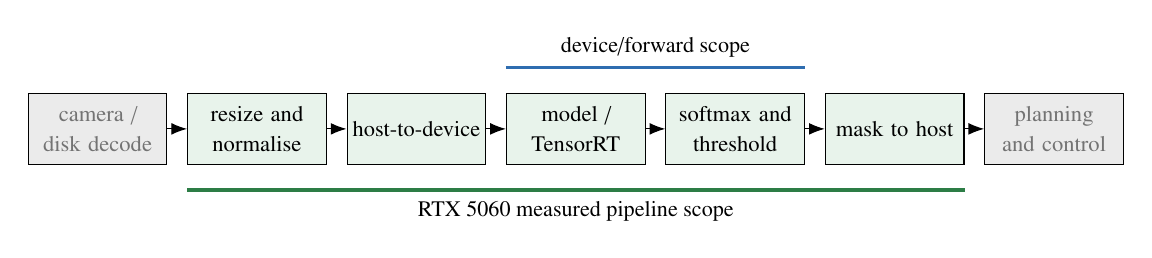
\begin{tikzpicture}[
  node distance=0.25cm,
  stage/.style={draw,minimum height=0.9cm,text width=1.62cm,align=center,font=\footnotesize,inner sep=2pt},
  included/.style={stage,fill=softgreen},
  excluded/.style={stage,fill=black!8,text=black!55},
  arrow/.style={-{Latex[length=2mm]},thin}
]
\node[excluded] (camera) {camera / disk decode};
\node[included,right=of camera] (resize) {resize and normalise};
\node[included,right=of resize] (h2d) {host-to-device};
\node[included,right=of h2d] (model) {model / TensorRT};
\node[included,right=of model] (post) {softmax and threshold};
\node[included,right=of post] (d2h) {mask to host};
\node[excluded,right=of d2h] (planner) {planning and control};
\draw[arrow] (camera) -- (resize);
\draw[arrow] (resize) -- (h2d);
\draw[arrow] (h2d) -- (model);
\draw[arrow] (model) -- (post);
\draw[arrow] (post) -- (d2h);
\draw[arrow] (d2h) -- (planner);
\draw[very thick,good] ($(resize.south west)+(0,-0.32)$) -- node[below,font=\footnotesize,text=black]{RTX~5060 measured pipeline scope} ($(d2h.south east)+(0,-0.32)$);
\draw[very thick,pidP] ($(model.north west)+(0,0.32)$) -- node[above,font=\footnotesize,text=black]{device/forward scope} ($(post.north east)+(0,0.32)$);
\end{tikzpicture}
}
\caption[Timing scopes used for the RTX 5060 benchmark.]{Timing scopes used for
the RTX~5060 benchmark. Grey stages are excluded. The device/forward scope
starts from GPU-resident input; the measured pipeline starts from an already
decoded host RGB array and returns a binary mask to host memory.}
\label{fig:timing_scopes}
\end{figure}

Figure~\ref{fig:timing_scopes} makes the two reported timing boundaries
explicit before their sample counts are introduced.

Timing uses 64 preloaded native-resolution test frames, ten excluded warm-up
passes, and five measured repeats, yielding 320 samples per model and scope.
The \emph{device scope} includes a device-to-device buffer copy, TensorRT
execution, softmax, and thresholding. It excludes host-to-device input and
device-to-host mask transfer. The \emph{measured pipeline} includes CPU resize
and normalisation, input transfer, TensorRT inference, softmax, thresholding,
and return of the mask to CPU memory. Both exclude disk decode, camera-driver
latency, visualisation, planning, actuation, and one-time engine construction.

After timing, each engine is evaluated on all 544 official test images. This
full accuracy pass is mandatory because mixed precision can move probabilities
across the 0.50 threshold even when average numerical differences are small.
TensorRT metrics are reported separately from the original PyTorch metrics.

\section{Artifact Provenance and Reproduction}

\noindent\textbf{Reproducibility repository:}\\
\url{https://github.com/hax2/cat-pidnet-thesis-reproducibility}. This public
repository is the companion artifact for the thesis. It contains the source
code, exact configurations, split and label-conversion records, experiment
launchers, checkpoint and metric evidence, audit scripts, and instructions
needed to reproduce the reported workflows. The appendix provides direct
commands and expected outputs so that the link is usable without having to
infer the execution order from the source tree.

A headline result is considered identified only when the following artifacts
are named:
\begin{enumerate}
  \item the processed split manifest and binary mapping;
  \item the complete YAML configuration;
  \item the selected \texttt{best.pt} checkpoint;
  \item the evaluator and metric implementation;
  \item the saved JSON result and, where applicable, hardware report.
\end{enumerate}

The reference PIDNet chain includes SHA-256 identities for all five elements and
for the qualitative review, CPU benchmark, ONNX model, TensorRT engine, and
TensorRT report. The saved test confusion matrix was independently recomputed
in a fresh CPU evaluation. Exact equality of the counts establishes
\emph{evaluation reproducibility}: the same artifact and evaluator produce the
same score. It is different from \emph{training repeatability}, which asks how
new stochastic training runs vary and is addressed only by the separate
three-seed studies.

The blue-only fixed-budget architecture ledger contains all 27 configurations,
metric records, and checkpoint hashes. The corresponding fixed-budget
blue+green ledger contains all 27 configuration and metric chains and all
confusion-derived integrity checks pass; 21 locally retained checkpoints have
hashes. The six earlier controlled PIDNet-S and ROD blue+green checkpoints
were not included in that download bundle.

The newer convergence-aware ledger is complete at the identity level: it
contains 27 configurations, histories, train summaries, test records, and
server-computed checkpoint SHA-256 values. All 27 confusion matrices reproduce
their reported metrics and each contains 133,693,440 evaluated pixels. The
checkpoint binaries themselves were not copied locally, so the ledger proves
their recorded server identity but does not permit local reevaluation without
retrieving a selected file.

The convergence campaign also records a software-stack limitation. PIDNet-S,
ROD, DDRNet, and BiSeNet ran with PyTorch 2.7.1 and CUDA 12.6, while the FPN,
U-Net, and SegFormer launcher used PyTorch 2.13.0 and CUDA 13.0 because its
environment contained the required SMP dependency. All used the same H100 MIG
partition, data, configurations, and metric implementation. The cross-model
ranking is usable as a recipe-level comparison, but framework version is not
fully controlled across architecture families.

Appendix~\ref{app:reproduction} gives commands and expected outputs.
Appendix~\ref{app:hashes} records the artifact identities. The repository ledgers
provide the per-seed architecture paths and integrity status.

% ============================================================
\chapter{Accuracy, Asymmetric Errors, and Qualitative Results}
\label{ch:results}
% ============================================================

\section{Reference PIDNet-S Result}

Table~\ref{tab:frozen_pidnet_result} reports the retained checkpoint on all 544
official test images. No image subset is used for the aggregate. This
artifact-level measurement is kept separate from the three-seed PIDNet mean,
which comes from a different training protocol.

\begin{table}[H]
\centering
\caption{Verified reference PIDNet-S result for blue+green traversability. Lower
FSR and FBR are preferable; the other quality metrics are higher-is-better.}
\label{tab:frozen_pidnet_result}
\begin{tabular}{@{}lr@{}}
\toprule
\textbf{Metric} & \textbf{Value} \\
\midrule
mIoU & \textbf{0.893941} \\
IoU untraversable & 0.908936 \\
IoU traversable & 0.878946 \\
Traversable precision & 0.941592 \\
Traversable recall & 0.929631 \\
Traversable F1 & 0.935573 \\
False-Safe Rate & \textbf{0.043176} (4.32\%) \\
False-Block Rate & \textbf{0.070369} (7.04\%) \\
Weighted cross-entropy test loss & 0.149528 \\
\bottomrule
\end{tabular}
\end{table}

Untraversable IoU is 3.00 percentage points higher than traversable IoU.
Traversable precision exceeds recall by 1.20 points, and FBR is 2.72 points
higher than FSR. At threshold 0.50, the model is therefore more likely to
remove an annotated traversable pixel than to open an annotated blocked pixel.
That conservative balance is visible numerically, but it does not prevent
large false-safe regions in individual images.

\begin{table}[H]
\centering
\caption{Aggregated pixel confusion matrix for the reference PIDNet-S checkpoint.
Rows are ground truth and columns are prediction.}
\label{tab:frozen_confusion}
\begin{tabular}{@{}llrr@{}}
\toprule
 & & \multicolumn{2}{c}{\textbf{Predicted}} \\
\cmidrule(lr){3-4}
 & & Untraversable & Traversable \\
\midrule
\multirow{2}{*}{\textbf{Ground truth}}
 & Untraversable & 73,151,244 (TN) & \textcolor{safety}{3,300,886 (FP)} \\
 & Traversable & \textcolor{block}{4,027,996 (FN)} & 53,213,314 (TP) \\
\bottomrule
\end{tabular}
\end{table}

Table~\ref{tab:frozen_confusion} exposes the four raw counts from which the
reference checkpoint's aggregate rates are calculated.

The matrix contains exactly
$544\times640\times384=133{,}693{,}440$ pixel decisions. Substitution into
Equations~\ref{eq:final_fsr} and \ref{eq:final_fbr} gives
\begin{align}
 \FSR&=\frac{3{,}300{,}886}{73{,}151{,}244+3{,}300{,}886}=0.043176,\\
 \FBR&=\frac{4{,}027{,}996}{53{,}213{,}314+4{,}027{,}996}=0.070369.
\end{align}
A fresh CPU evaluation reproduced all four counts and every derived metric
exactly. This direct calculation also prevents the two denominators from being
accidentally interchanged.

\section{PIDNet--ROD Comparison}

Under the matched three-seed blue+green recipe, ROD reaches
$0.9138\pm0.0003$ mIoU compared with $0.8822\pm0.0002$ for PIDNet-S. The
reported difference is 3.15 percentage points using the unrounded run values.
ROD also reduces mean FSR from 4.98\% to 3.51\% and mean FBR from 7.67\% to
5.62\%. Under blue-only, ROD reaches $0.9211\pm0.0010$ versus
$0.8832\pm0.0016$ for PIDNet-S, a 3.79-point improvement, while reducing both
asymmetric rates.

The small observed ROD standard deviations and the size of the mean gaps show
that its advantage over PIDNet-S is not explained by one favourable seed: ROD records
the higher test mIoU in every one of the six policy--seed runs. Because
ROD simultaneously changes architecture, pretraining, normalisation, internal
resolution, and trainable-parameter allocation, the experiment does not show
which component causes the improvement. It establishes that the complete ROD
pipeline achieves higher CaT accuracy than the matched PIDNet pipeline.

The closest documented ROD recipe improves further
(Table~\ref{tab:rod_paper_results}). For blue+green, mIoU rises by 0.98 points
over the controlled ROD mean. FSR is 0.34 points higher, but FBR falls by 1.65
points, so much of the gain reflects better recovery of traversable pixels
rather than uniformly more conservative prediction. For blue-only, both
reported error rates improve relative to controlled ROD.

\begin{table}[H]
\centering
\caption{Closest documented ROD recipe transferred to CaT. This is a
single-seed approximation because the publication omits the epoch budget and
augmentation policy.}
\label{tab:rod_paper_results}
\small
\begin{tabular}{@{}lrrrrrr@{}}
\toprule
\textbf{Policy} & \textbf{mIoU} & \textbf{IoU untrav.} & \textbf{IoU trav.} & \textbf{F1} & \textbf{FSR} & \textbf{FBR} \\
\midrule
Blue+green & 0.9236 & 0.9338 & 0.9134 & 0.9547 & 3.85\% & 3.97\% \\
Blue-only & 0.9280 & 0.9590 & 0.8970 & 0.9457 & 2.20\% & 5.14\% \\
\bottomrule
\end{tabular}
\end{table}

These experiments establish a repeatable advantage over PIDNet-S. Whether that
advantage is competitive with other compact systems is answered by the
nine-model comparison.

\section{Fixed-Budget Blue+Green Architecture Comparison}

Table~\ref{tab:wider_blue_green} gives the nine-model result for the
blue+green policy after the original common budget of 15 epochs. The FPN with
an EfficientNet-B0 encoder has the highest
observed mean mIoU at 93.15\%; the corresponding U-Net records 93.13\%.
Both have a population standard deviation of 0.07 percentage points across
the three runs, whereas their means differ by only 0.02 points. With only
three runs, the data support a common leading performance band but not a
reliable ordering of the two decoders.

\begin{table}[H]
\centering
\caption{Fixed-15-epoch blue+green results over seeds 1337, 2027, and 4242
(mean $\pm$ population standard deviation). Lower FSR and FBR are preferable.}
\label{tab:wider_blue_green}
\footnotesize
\setlength{\tabcolsep}{4pt}
\begin{tabular}{@{}lrrrr@{}}
\toprule
\textbf{Model} & \textbf{mIoU} & \textbf{F1} & \textbf{FSR} & \textbf{FBR} \\
\midrule
\textbf{FPN/EfficientNet-B0} & $\mathbf{0.9315\pm0.0007}$ & $\mathbf{0.9594\pm0.0005}$ & $0.0293\pm0.0013$ & $\mathbf{0.0420\pm0.0021}$ \\
\textbf{U-Net/EfficientNet-B0} & $\mathbf{0.9313\pm0.0007}$ & $\mathbf{0.9592\pm0.0004}$ & $\mathbf{0.0288\pm0.0007}$ & $0.0429\pm0.0016$ \\
FPN/MobileNetV2 & $0.9255\pm0.0001$ & $0.9556\pm0.0001$ & $0.0309\pm0.0013$ & $0.0472\pm0.0015$ \\
SegFormer-B0 & $0.9254\pm0.0002$ & $0.9555\pm0.0001$ & $0.0296\pm0.0008$ & $0.0491\pm0.0009$ \\
U-Net/MobileNetV2 & $0.9207\pm0.0016$ & $0.9528\pm0.0009$ & $0.0374\pm0.0029$ & $0.0446\pm0.0019$ \\
ROD ViT-S & $0.9138\pm0.0003$ & $0.9482\pm0.0003$ & $0.0351\pm0.0028$ & $0.0562\pm0.0038$ \\
BiSeNetV2 & $0.8868\pm0.0007$ & $0.9307\pm0.0005$ & $0.0425\pm0.0039$ & $0.0803\pm0.0048$ \\
PIDNet-S & $0.8822\pm0.0002$ & $0.9281\pm0.0002$ & $0.0498\pm0.0043$ & $0.0767\pm0.0053$ \\
DDRNet-23-Slim & $0.8746\pm0.0063$ & $0.9228\pm0.0042$ & $0.0499\pm0.0020$ & $0.0862\pm0.0062$ \\
\bottomrule
\end{tabular}
\end{table}

Relative to PIDNet-S, FPN/EfficientNet-B0 improves mean mIoU by 4.93 points,
reduces FSR by 2.05 points, and reduces FBR by 3.47 points. The gain is not
merely a threshold shift from one error direction to the other. U-Net with the
same encoder has nearly identical accuracy and the lowest observed mean FSR.
FPN has slightly lower FBR. With three seeds, those small differences support
a shared performance tier rather than selecting one decoder universally.

The $2\times2$ encoder--decoder subset shows two consistent patterns.
EfficientNet-B0 improves mean mIoU over MobileNetV2 with either FPN or U-Net,
and FPN improves mean mIoU over U-Net with either encoder. The decoder effect
is much smaller with EfficientNet-B0 than with MobileNetV2. SegFormer-B0 has
nearly the same mean mIoU as FPN/MobileNetV2. ROD ranks sixth in this
controlled table: substantially above PIDNet-S, BiSeNetV2, and DDRNet, but
below the four generic encoder--decoder systems and SegFormer-B0.

The single-seed ROD paper recipe reaches 92.36\%, which narrows the gap but
still remains below the 93.15\% and 93.13\% three-seed means of the top
controlled systems. Since its optimiser, loss, augmentation, and seed protocol
differ, that observation is descriptive rather than a strict row-wise
comparison.

\section{Convergence-Aware Blue+Green Follow-Up}

The fixed-budget table controls training exposure, but it does not show what
the same recipes reach after their validation curves flatten. The follow-up
therefore keeps the blue+green data, loss, augmentation, optimiser, initial
learning rate, threshold, and three seeds fixed while extending the training
horizon. The 300 epochs are a ceiling. No run reaches it: early stopping ends
the 27 runs between epochs 74 and 150, and validation selects checkpoints
between epochs 50 and 141.

Table~\ref{tab:convergence_blue_green} reports the resulting test metrics. The
selected epochs are listed in seed order 1337, 2027, and 4242. They are part of
the result because replacing them with one round number would conceal large
between-model and between-seed differences.

\begin{table}[H]
\centering
\caption[Convergence-aware blue+green architecture results.]{Convergence-aware
blue+green results over seeds 1337, 2027, and 4242. Each metric cell places
the mean above its $\pm$ population standard deviation. ``Selected epochs''
gives the validation-selected \texttt{best.pt} epoch for those three seeds.
Lower FSR and FBR are preferable.}
\label{tab:convergence_blue_green}
\footnotesize
\setlength{\tabcolsep}{4pt}
\renewcommand{\arraystretch}{1.08}
\newcommand{\resultcell}[2]{\shortstack{$#1$\\[-1pt]{\scriptsize$\pm #2$}}}
\begin{tabular*}{\textwidth}{@{\extracolsep{\fill}}lccccc@{}}
\toprule
\textbf{Model} & \textbf{Selected epochs} & \textbf{mIoU} & \textbf{F1} & \textbf{FSR} & \textbf{FBR} \\
\midrule
\textbf{FPN/EfficientNet-B0} & 119/90/83 & \resultcell{\mathbf{0.9423}}{\mathbf{0.0005}} & \resultcell{\mathbf{0.9660}}{\mathbf{0.0003}} & \resultcell{\mathbf{0.0255}}{\mathbf{0.0004}} & \resultcell{\mathbf{0.0340}}{\mathbf{0.0011}} \\
U-Net/EfficientNet-B0 & 102/76/56 & \resultcell{0.9409}{0.0004} & \resultcell{0.9652}{0.0002} & \resultcell{0.0260}{0.0002} & \resultcell{0.0349}{0.0003} \\
FPN/MobileNetV2 & 70/99/65 & \resultcell{0.9372}{0.0005} & \resultcell{0.9629}{0.0003} & \resultcell{0.0274}{0.0003} & \resultcell{0.0376}{0.0010} \\
SegFormer-B0 & 50/141/87 & \resultcell{0.9341}{0.0005} & \resultcell{0.9610}{0.0003} & \resultcell{0.0304}{0.0004} & \resultcell{0.0374}{0.0002} \\
U-Net/MobileNetV2 & 74/79/57 & \resultcell{0.9332}{0.0004} & \resultcell{0.9605}{0.0002} & \resultcell{0.0314}{0.0001} & \resultcell{0.0372}{0.0005} \\
ROD ViT-S & 74/82/54 & \resultcell{0.9331}{0.0004} & \resultcell{0.9604}{0.0002} & \resultcell{0.0294}{0.0005} & \resultcell{0.0399}{0.0003} \\
PIDNet-S & 104/75/75 & \resultcell{0.9195}{0.0029} & \resultcell{0.9519}{0.0018} & \resultcell{0.0335}{0.0013} & \resultcell{0.0511}{0.0019} \\
BiSeNetV2 & 125/58/123 & \resultcell{0.9149}{0.0019} & \resultcell{0.9490}{0.0012} & \resultcell{0.0361}{0.0021} & \resultcell{0.0536}{0.0020} \\
DDRNet-23-Slim & 81/68/93 & \resultcell{0.9095}{0.0022} & \resultcell{0.9456}{0.0014} & \resultcell{0.0374}{0.0009} & \resultcell{0.0584}{0.0017} \\
\bottomrule
\end{tabular*}
\end{table}

FPN/EfficientNet-B0 has the highest mean mIoU and also the lowest mean FSR and
FBR. It scores above U-Net/EfficientNet-B0 in each matched seed; the mean lead
is 0.13 percentage points. This is a consistent first place within the 27
executed runs, although three seeds and one split do not establish a universal
decoder ranking. The two MobileNetV2 decoders separate more clearly:
FPN/MobileNetV2 leads U-Net/MobileNetV2 by 0.41 points. ROD and
U-Net/MobileNetV2 differ by only 0.003 percentage points in mean mIoU, far
below either model's observed between-seed standard deviation, but retain
different error balances.

\begin{figure}[H]
\centering
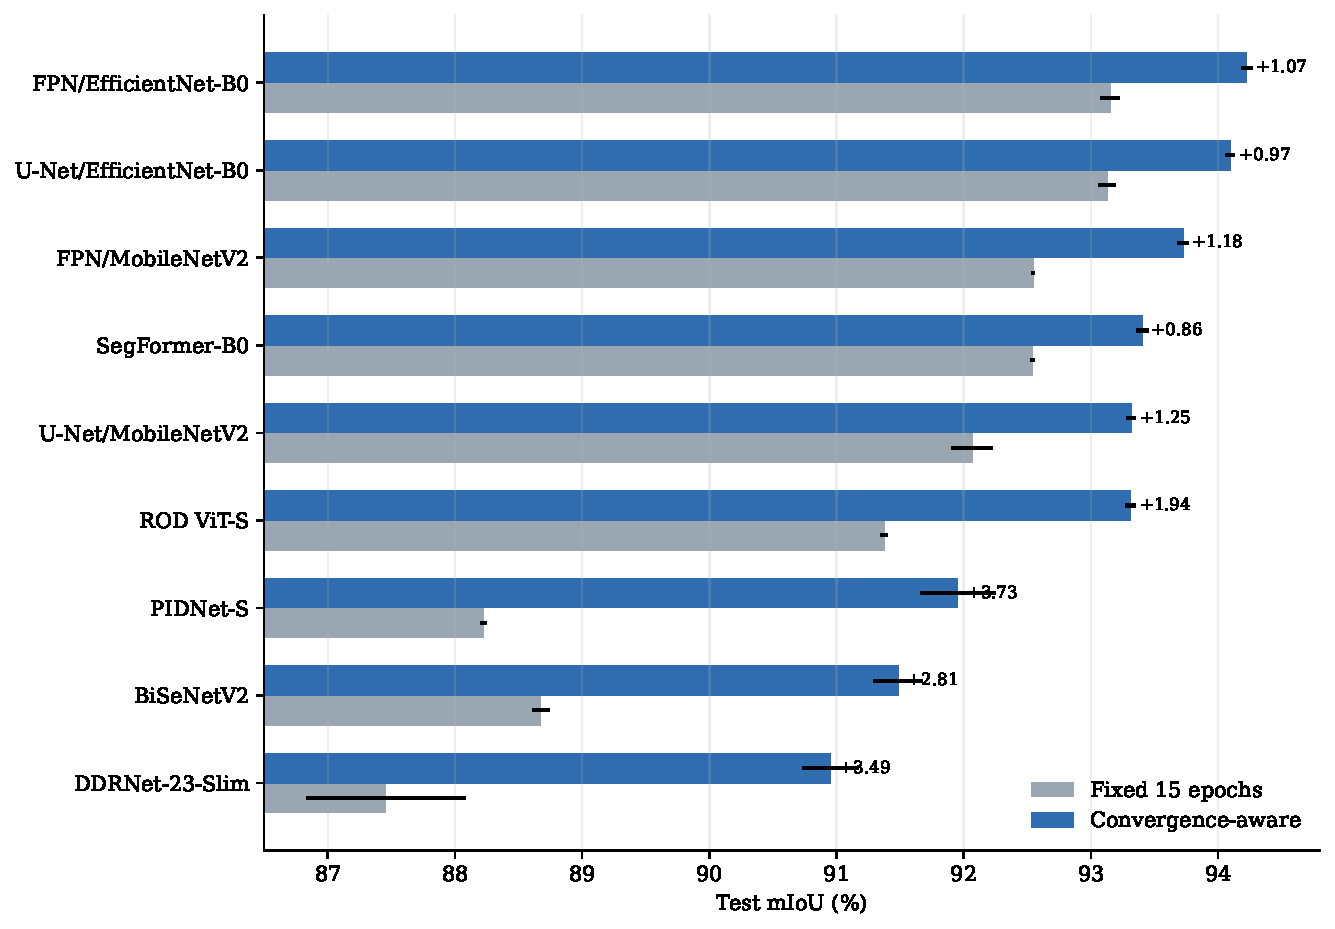
\includegraphics[width=0.98\textwidth]{figures/generated/convergence_miou_comparison.pdf}
\caption[Fixed-budget and convergence-aware test mIoU.]{Mean test mIoU under
the fixed 15-epoch and convergence-aware blue+green protocols. Error bars are
population standard deviations over three seeds; labels give the change in
percentage points. Every architecture improves, but the size of the gain is
strongly model-dependent.}
\label{fig:convergence_miou_comparison}
\end{figure}

Figure~\ref{fig:convergence_miou_comparison} shows that the extended protocol
does not merely add a common offset. PIDNet-S gains 3.73 points,
DDRNet-23-Slim 3.49, and BiSeNetV2 2.81, whereas the two EfficientNet-B0
systems gain about one point. The earlier comparison therefore penalised the
slower-converging real-time models most strongly. Since the follow-up was run
later and used two recorded PyTorch environments across architecture groups,
the exact differences are protocol-level changes rather than pure causal
estimates of additional epochs alone.

\begin{figure}[H]
\centering
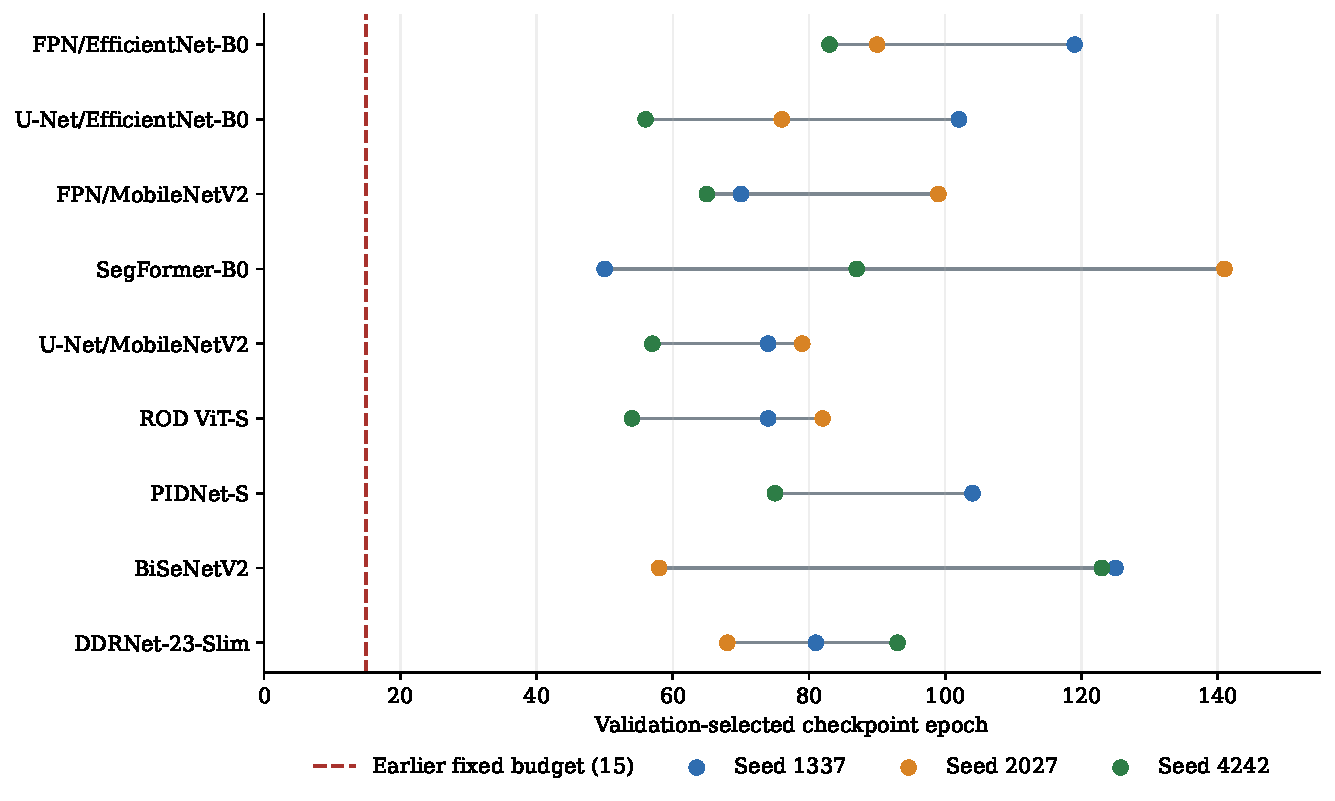
\includegraphics[width=0.98\textwidth]{figures/generated/convergence_selected_epochs.pdf}
\caption[Validation-selected epochs in the convergence suite.]{Checkpoint
epochs selected by validation mIoU. The dashed line marks the earlier
15-epoch budget. Horizontal segments span the three seeds of one architecture;
none of the 27 selected checkpoints lies near epoch 15.}
\label{fig:convergence_selected_epochs}
\end{figure}

Figure~\ref{fig:convergence_selected_epochs} shows both between-model and
between-seed variation in the validation-selected checkpoint epoch.

The selected epochs range from 50 for one SegFormer run to 141 for another.
This spread is the direct reason not to replace the fixed budget with a claim
that one epoch count, such as 60 or 300, is ``optimal'' for every model. The
curves in Figure~\ref{fig:convergence_validation_curves} add the missing
temporal context: pretrained encoder--decoders rise quickly but continue to
make small gains, while PIDNet, BiSeNet, and DDRNet require a longer initial
climb.

\begin{figure}[H]
\centering
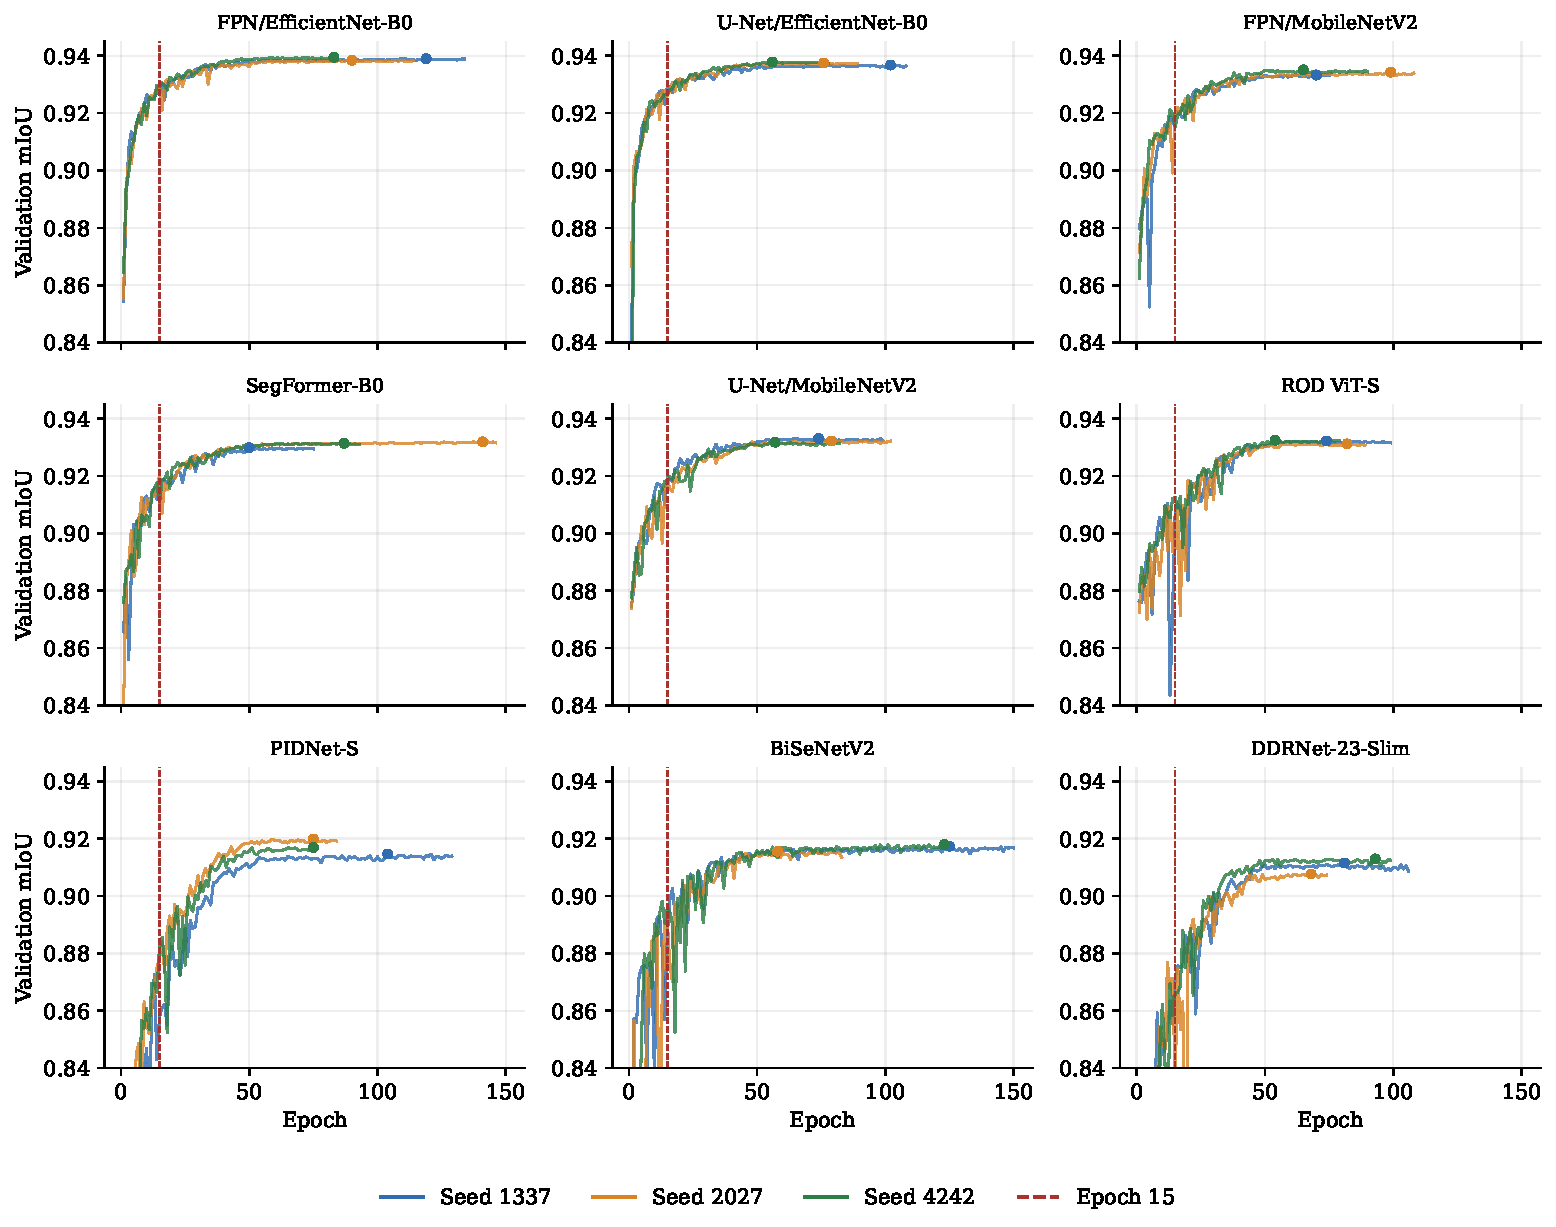
\includegraphics[width=\textwidth]{figures/generated/convergence_validation_curves.pdf}
\caption[Validation histories for the convergence-aware runs.]{Validation
mIoU histories for all 27 convergence-aware runs. Dots mark the saved maximum
for each seed and the dashed line marks epoch 15. The histories support a
longer protocol, but their late fluctuations also show why validation-based
checkpoint selection is preferable to reporting the final epoch.}
\label{fig:convergence_validation_curves}
\end{figure}

\section{Blue-Only Architecture Comparison}

The blue-only table shows the same broad ordering. The task is different, so
its higher mIoU values should not be interpreted as a direct improvement over
blue+green. The EfficientNet-B0 FPN and U-Net again form the top tier: their
means differ by 0.04 points, comparable to their observed 0.05--0.06-point seed
variation.

Table~\ref{tab:wider_blue_only} reports this fixed-budget blue-only matrix in
full; it is not merged with the convergence-aware blue+green evidence.

\begin{table}[H]
\centering
\caption{Controlled blue-only results over seeds 1337, 2027, and 4242
(mean $\pm$ population standard deviation). Lower FSR and FBR are preferable.}
\label{tab:wider_blue_only}
\footnotesize
\setlength{\tabcolsep}{4pt}
\begin{tabular}{@{}lrrrr@{}}
\toprule
\textbf{Model} & \textbf{mIoU} & \textbf{F1} & \textbf{FSR} & \textbf{FBR} \\
\midrule
\textbf{FPN/EfficientNet-B0} & $\mathbf{0.9376\pm0.0006}$ & $\mathbf{0.9531\pm0.0005}$ & $\mathbf{0.0180\pm0.0007}$ & $0.0469\pm0.0016$ \\
\textbf{U-Net/EfficientNet-B0} & $\mathbf{0.9372\pm0.0005}$ & $\mathbf{0.9529\pm0.0004}$ & $0.0192\pm0.0013$ & $\mathbf{0.0445\pm0.0028}$ \\
FPN/MobileNetV2 & $0.9332\pm0.0009$ & $0.9497\pm0.0007$ & $0.0193\pm0.0015$ & $0.0502\pm0.0040$ \\
SegFormer-B0 & $0.9286\pm0.0013$ & $0.9461\pm0.0010$ & $0.0214\pm0.0008$ & $0.0523\pm0.0011$ \\
U-Net/MobileNetV2 & $0.9283\pm0.0001$ & $0.9460\pm0.0000$ & $0.0233\pm0.0017$ & $0.0479\pm0.0040$ \\
ROD ViT-S & $0.9211\pm0.0010$ & $0.9401\pm0.0008$ & $0.0230\pm0.0013$ & $0.0597\pm0.0019$ \\
BiSeNetV2 & $0.8885\pm0.0026$ & $0.9140\pm0.0020$ & $0.0363\pm0.0028$ & $0.0788\pm0.0052$ \\
PIDNet-S & $0.8832\pm0.0016$ & $0.9093\pm0.0014$ & $0.0353\pm0.0016$ & $0.0897\pm0.0039$ \\
DDRNet-23-Slim & $0.8743\pm0.0042$ & $0.9019\pm0.0039$ & $0.0384\pm0.0022$ & $0.0963\pm0.0116$ \\
\bottomrule
\end{tabular}
\end{table}

The best blue-only systems reach lower FSR than under blue+green because the
negative class is larger and the target boundary changes; the numerical rates
remain policy-specific. ROD retains its advantage over PIDNet-S but again ranks
below the five strongest compact alternatives. DDRNet's larger standard
deviation shows that not every architecture is equally stable under the
15-epoch recipe.

For literature context, the reconstructed ROD blue-only traversable IoU is
89.70\%, while the original CaT PSPNet/ResNet-101 sedan IoU is 91.65\%
~\cite{sharma2022cat}. The positive pixel identity is aligned, but one model is
trained as binary segmentation and the other as four-class segmentation, so
the 1.95-point gap is contextual rather than a controlled architecture
comparison.

\section{High-Performing PIDNet Cases}

Figure~\ref{fig:pidnet_successes} presents the four PIDNet cases with the
lowest per-image sum of FSR and FBR. Each triptych shows the RGB image, ground
truth, and prediction. The two open-field examples demonstrate that the
model can reproduce a nearly horizontal transition between a foreground
vehicle-capability region and a distant blocked field even when both are pale
and textured. The wooded-trail example recovers a narrowing corridor and its
asymmetric edges. The curved open-track example follows a broad bend while
leaving a small interior blocked island.

\begin{figure}[H]
\centering
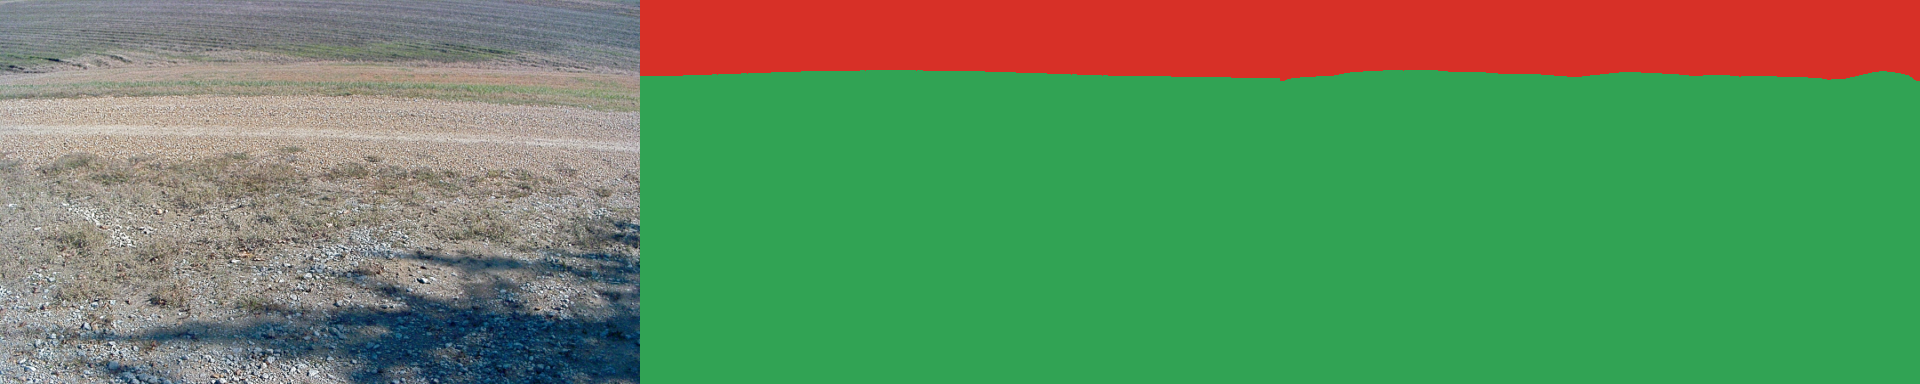
\includegraphics[width=0.48\linewidth]{figures/qualitative/pidnet_success_mixed_pln_1311.png}
\hfill
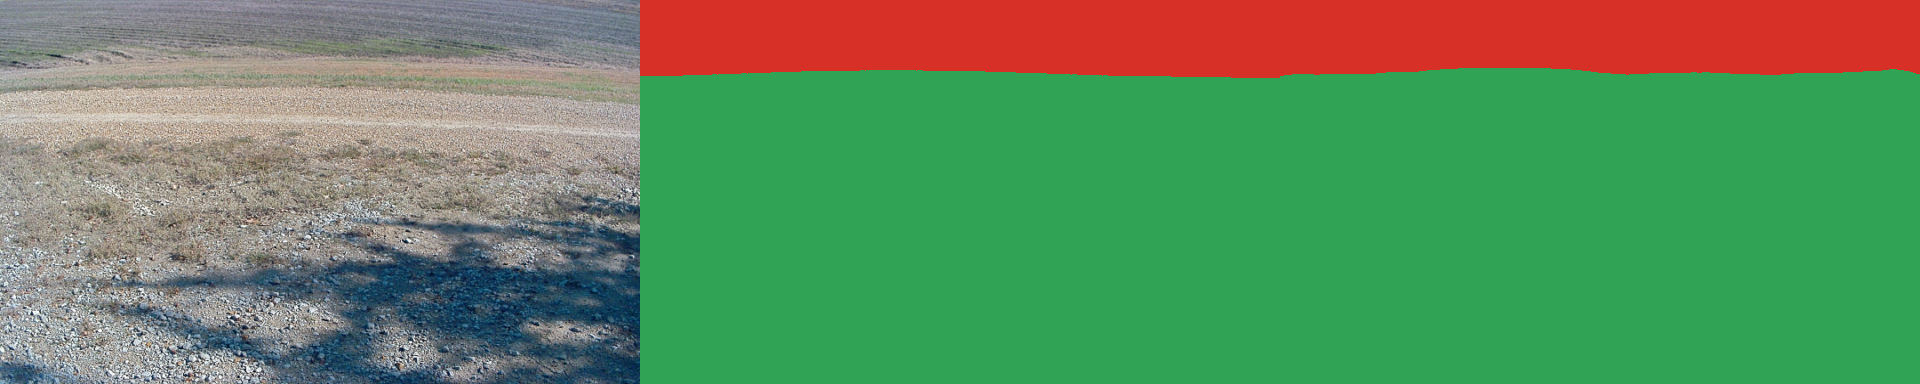
\includegraphics[width=0.48\linewidth]{figures/qualitative/pidnet_success_mixed_pln_1306.png}

\vspace{0.2cm}
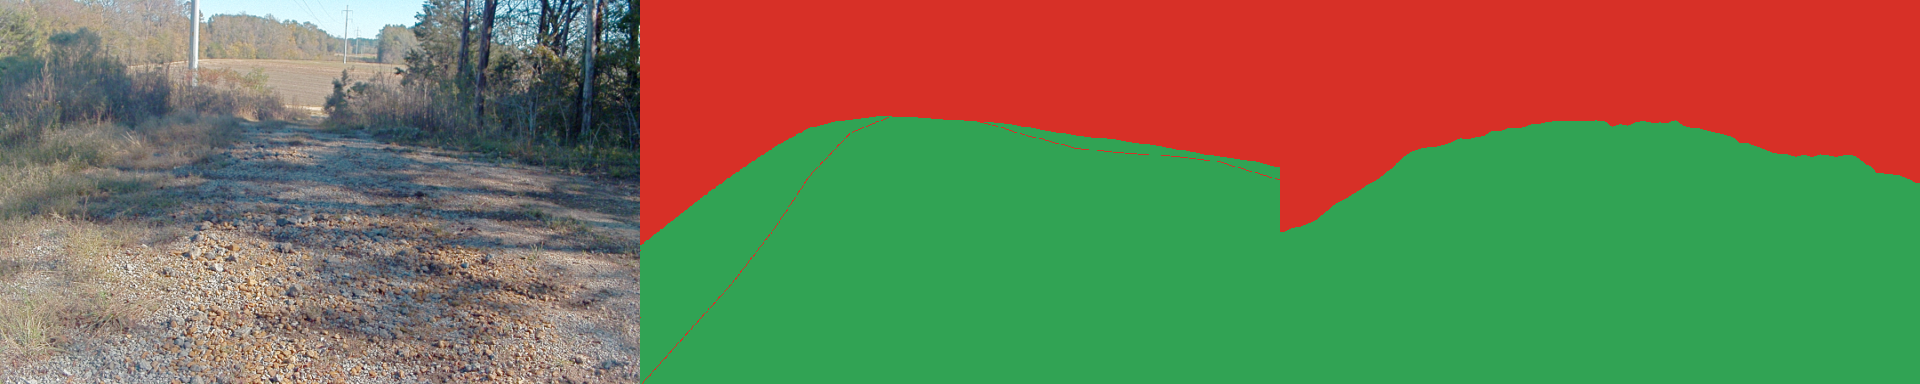
\includegraphics[width=0.48\linewidth]{figures/qualitative/pidnet_success_mixed_pln_1188.png}
\hfill
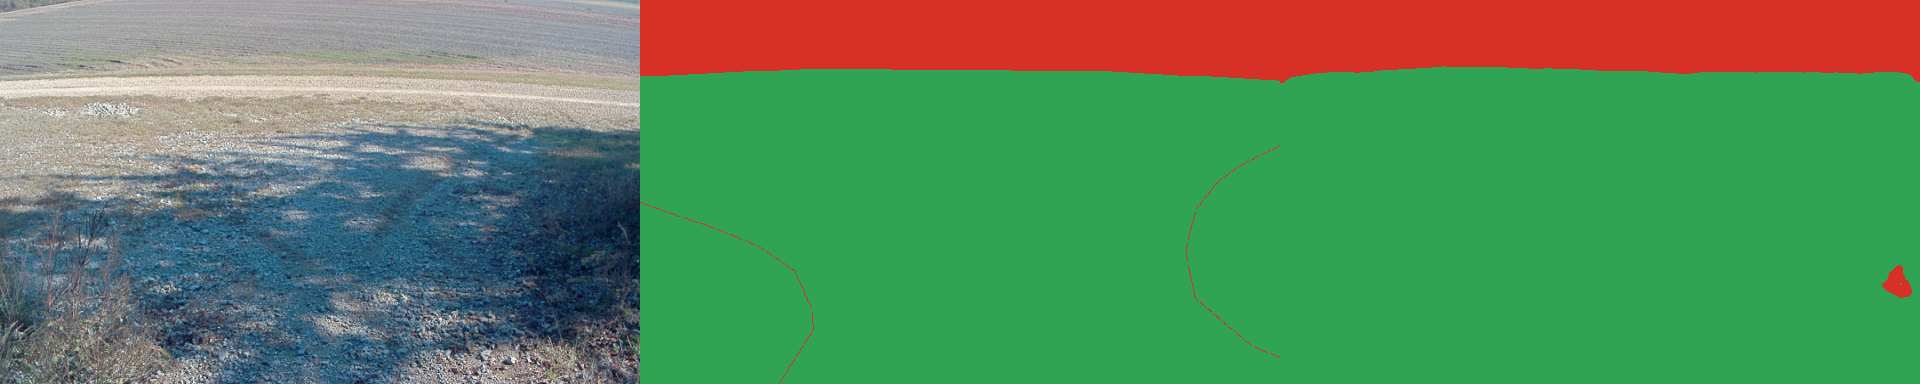
\includegraphics[width=0.48\linewidth]{figures/qualitative/pidnet_success_mixed_pln_1282.png}
\caption[High-performing reference PIDNet-S examples.]{High-performing
reference PIDNet-S examples selected by the lowest per-image sum of FSR and FBR. Each
triptych is RGB, binary ground truth, and prediction. Green denotes
traversable; red denotes untraversable. These are reproducible successes, not
a representative sample of the complete test distribution.}
\label{fig:pidnet_successes}
\end{figure}

The similarity between the ground-truth and prediction panels in these cases
shows that the model is learning a region-level task, not merely detecting a
central road centreline. It predicts the full visible capability envelope and
responds to distant boundary shape. Selection by low error also means these
images cannot be used to infer how often such behaviour occurs.

\section{Performance Across the Test Distribution}

Figure~\ref{fig:pidnet_percentiles} spans the 10th to 90th percentiles of
combined per-image error. The top winding-track image recovers a broad
connected corridor with small contour differences. By the 70th percentile the
prediction narrows the visible region, and the 90th-percentile woodland case
blocks much of a weakly defined corridor.

\begin{figure}[H]
\centering
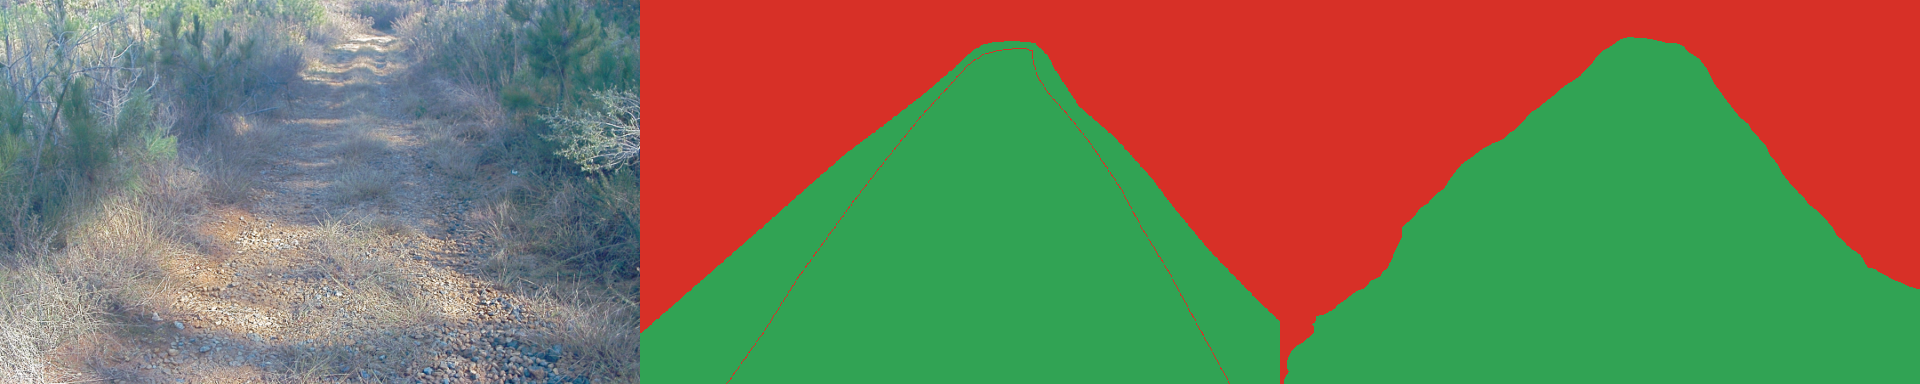
\includegraphics[width=0.96\linewidth]{figures/qualitative/pidnet_percentile_10_mixed_pln_961.png}

\vspace{0.12cm}
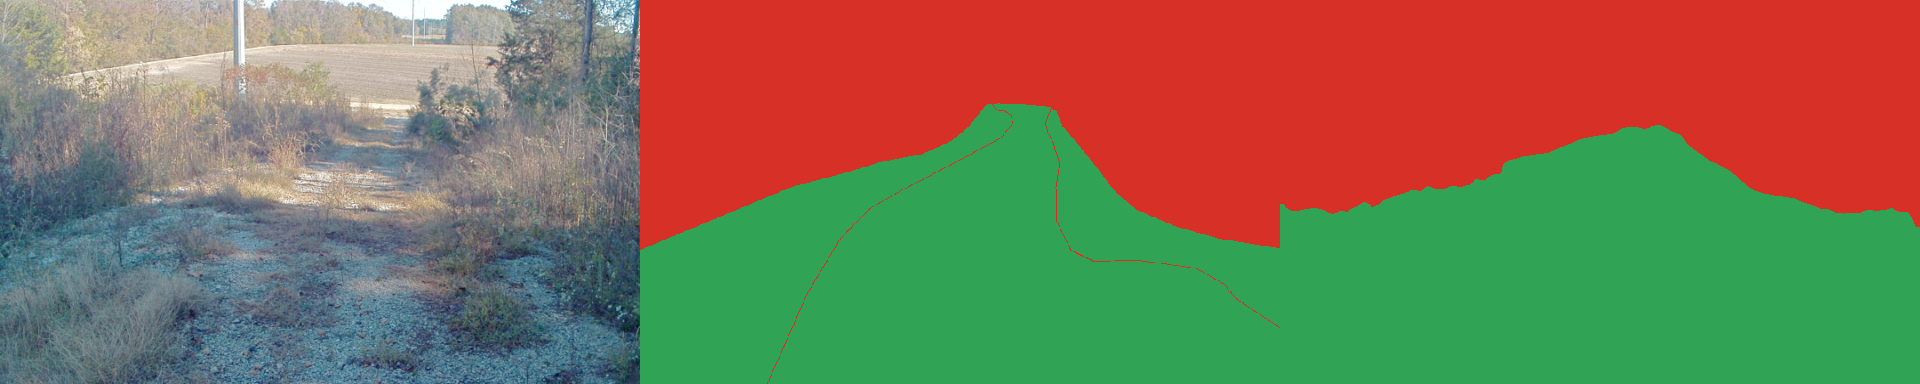
\includegraphics[width=0.96\linewidth]{figures/qualitative/pidnet_percentile_30_mixed_pln_1209.png}

\vspace{0.12cm}
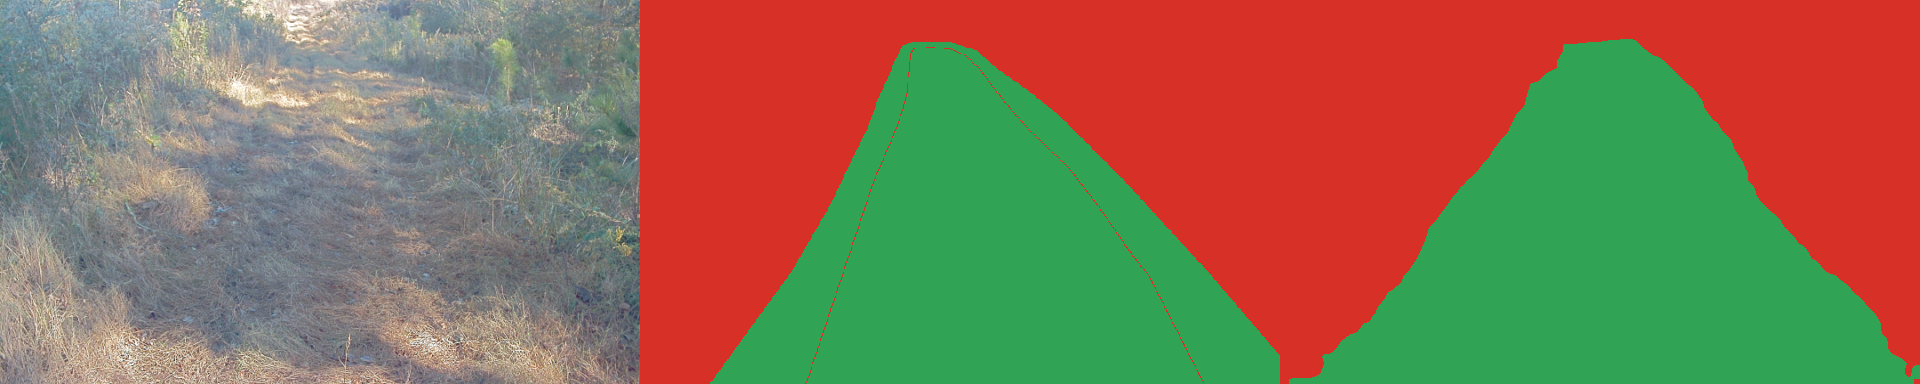
\includegraphics[width=0.96\linewidth]{figures/qualitative/pidnet_percentile_50_mixed_pln_119.png}

\vspace{0.12cm}
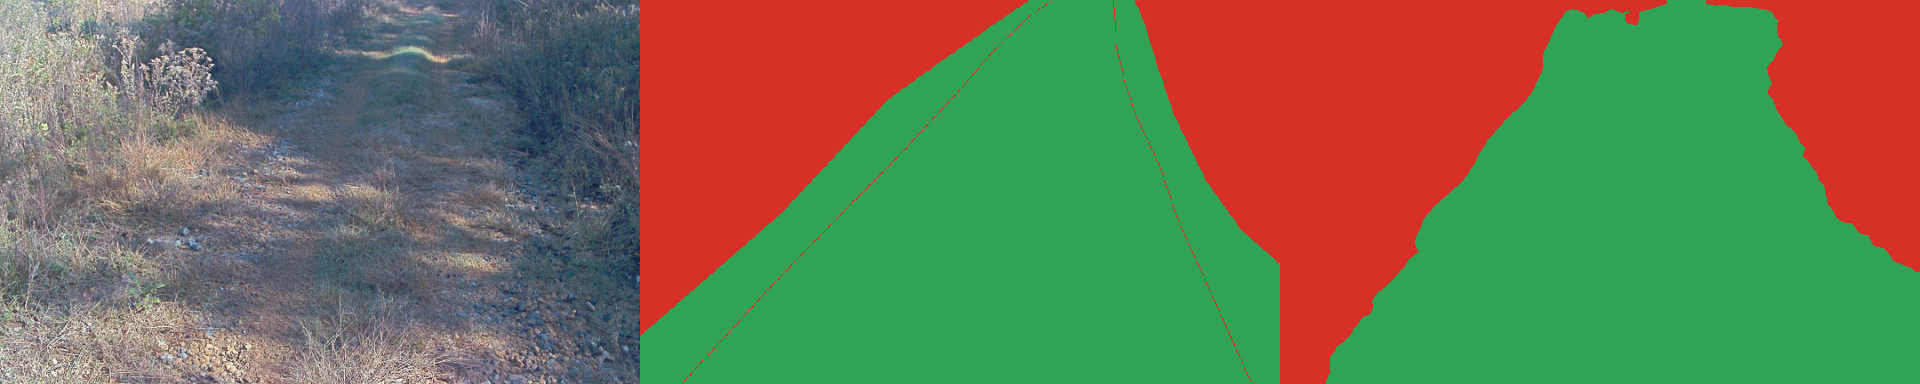
\includegraphics[width=0.96\linewidth]{figures/qualitative/pidnet_percentile_70_mixed_pln_1033.png}

\vspace{0.12cm}
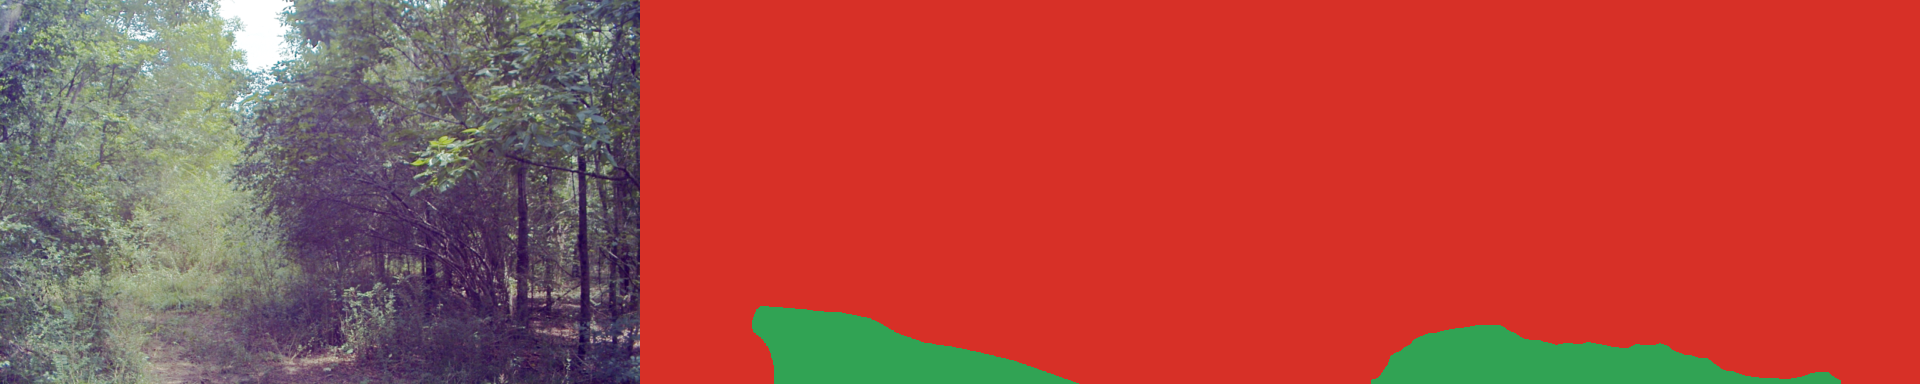
\includegraphics[width=0.96\linewidth]{figures/qualitative/pidnet_percentile_90_mixed_89.png}
\caption[PIDNet-S predictions across the test performance range.]{Reference
PIDNet-S predictions at the 10th, 30th, 50th, 70th, and 90th percentiles of
per-image $\FSR+\FBR$, from top to bottom. Each triptych is RGB, ground truth,
and prediction. The corresponding (FSR, FBR) pairs are (3.51\%, 2.47\%),
(5.92\%, 2.71\%), (6.90\%, 4.20\%), (5.27\%, 9.67\%), and
(1.62\%, 19.75\%).}
\label{fig:pidnet_percentiles}
\end{figure}

The sequence explains why one per-image scalar is incomplete. The
50th-percentile image is weighted toward false-safe error, while the
90th-percentile image has a low FSR but a 19.75\% FBR. Both may occupy a
similar rank under a combined score while requiring different remedies.

\begin{figure}[H]
\centering
\begin{subfigure}[t]{0.78\linewidth}
  \centering
  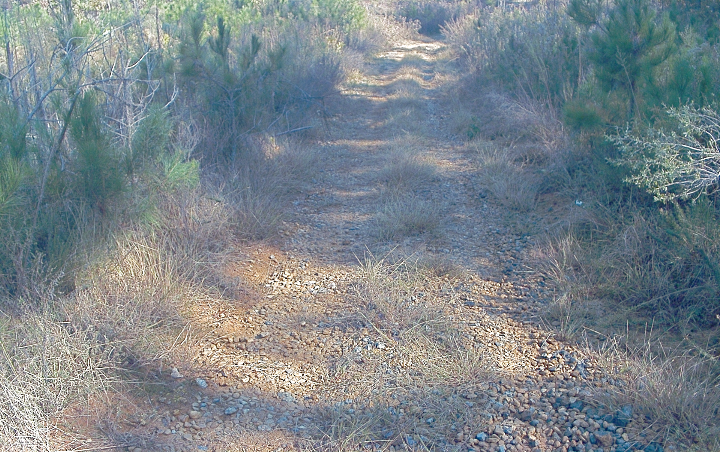
\includegraphics[width=\linewidth]{figures/qualitative/pidnet_detail_mixed_pln_961_rgb.png}
  \caption{RGB input.}
\end{subfigure}

\vspace{0.18cm}
\begin{subfigure}[t]{0.485\linewidth}
  \centering
  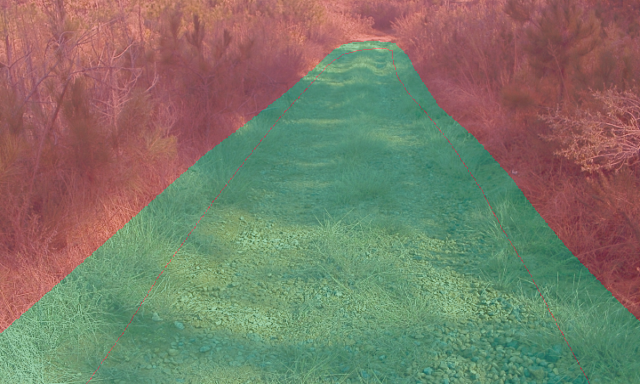
\includegraphics[width=\linewidth]{figures/qualitative/pidnet_detail_mixed_pln_961_gt.png}
  \caption{Ground-truth mapping.}
\end{subfigure}\hfill
\begin{subfigure}[t]{0.485\linewidth}
  \centering
  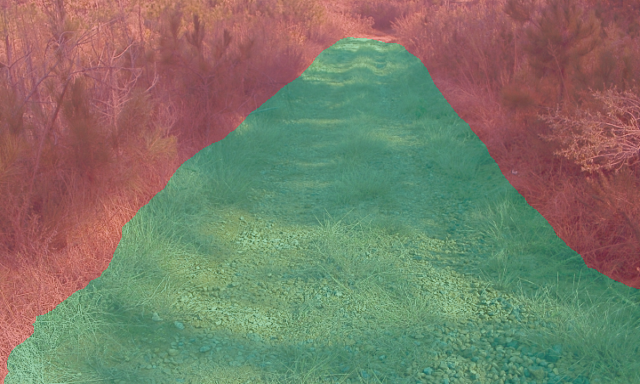
\includegraphics[width=\linewidth]{figures/qualitative/pidnet_detail_mixed_pln_961_prediction.png}
  \caption{PIDNet-S prediction.}
\end{subfigure}
\caption[Detailed successful winding-track example.]{Detailed view of
\texttt{mixed\_pln\_961}, the 10th-percentile example. The model follows the
winding foreground corridor into the distance. Its remaining 3.51\% FSR and
2.47\% FBR are concentrated primarily along the two lateral boundaries.}
\label{fig:pidnet_mapping_overlay}
\end{figure}

In Figure~\ref{fig:pidnet_mapping_overlay}, green extends along the track while
vegetation and terrain outside the selected vehicle envelope remain red. The
ground-truth and prediction overlays make small boundary offsets visible that
are difficult to see in the binary panels alone. The image connects the low
per-image rates to their spatial form.

\section{False-Safe, False-Block, and Boundary Failures}

\begin{figure}[H]
\centering
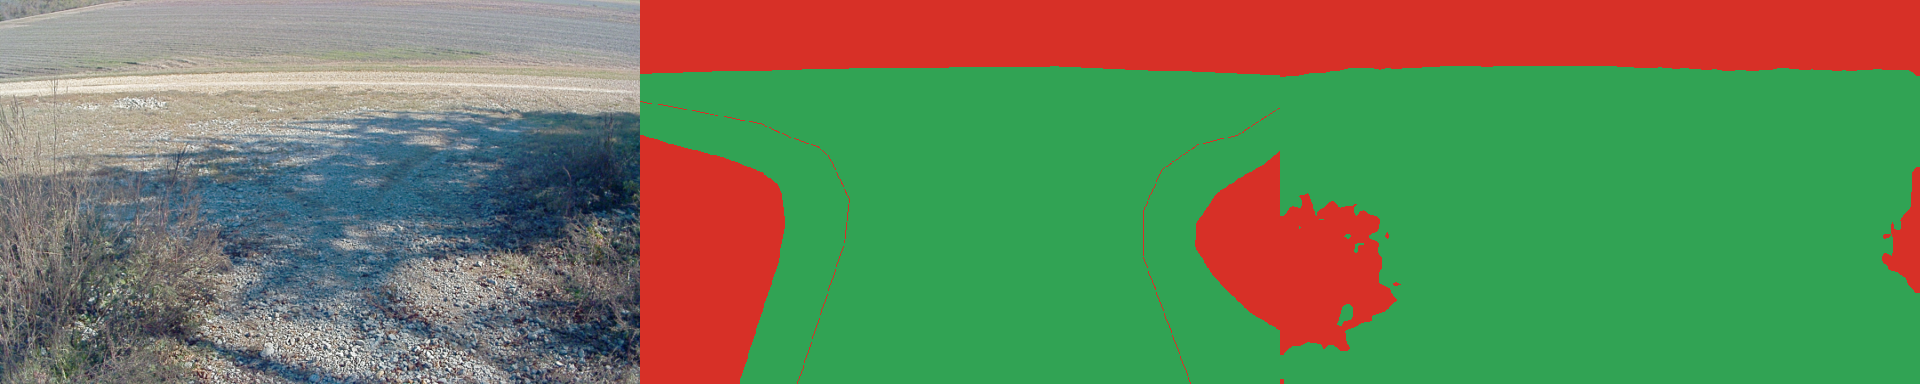
\includegraphics[width=0.96\linewidth]{figures/qualitative/pidnet_failure_false_safe_mixed_pln_1278.png}

\vspace{0.16cm}
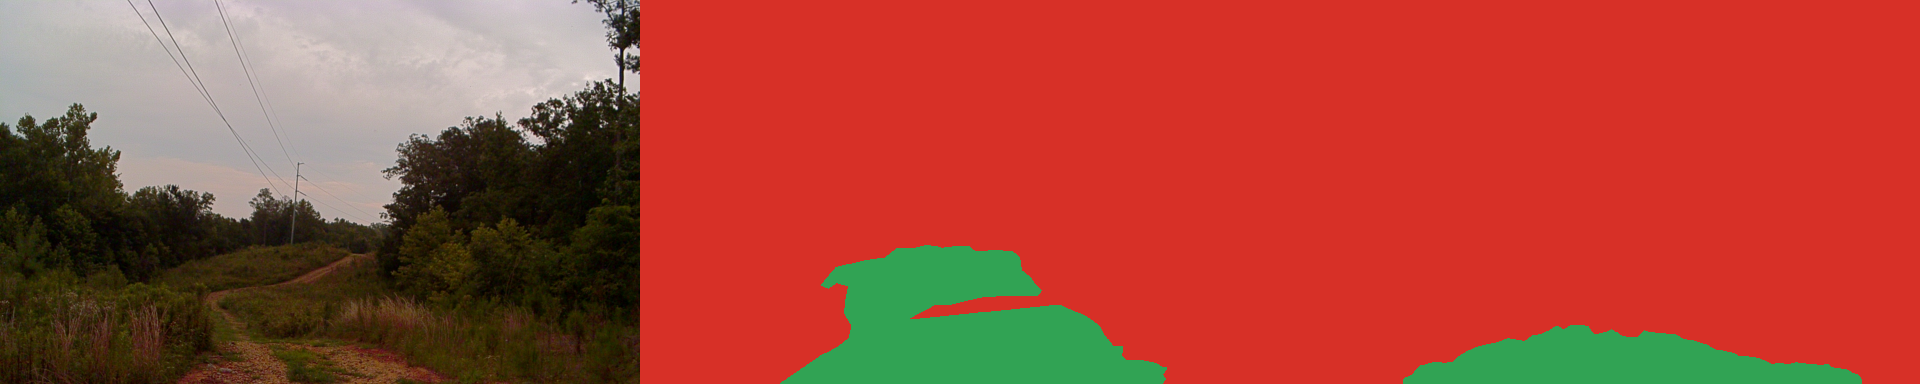
\includegraphics[width=0.96\linewidth]{figures/qualitative/pidnet_failure_false_block_mixed_425.png}

\vspace{0.16cm}
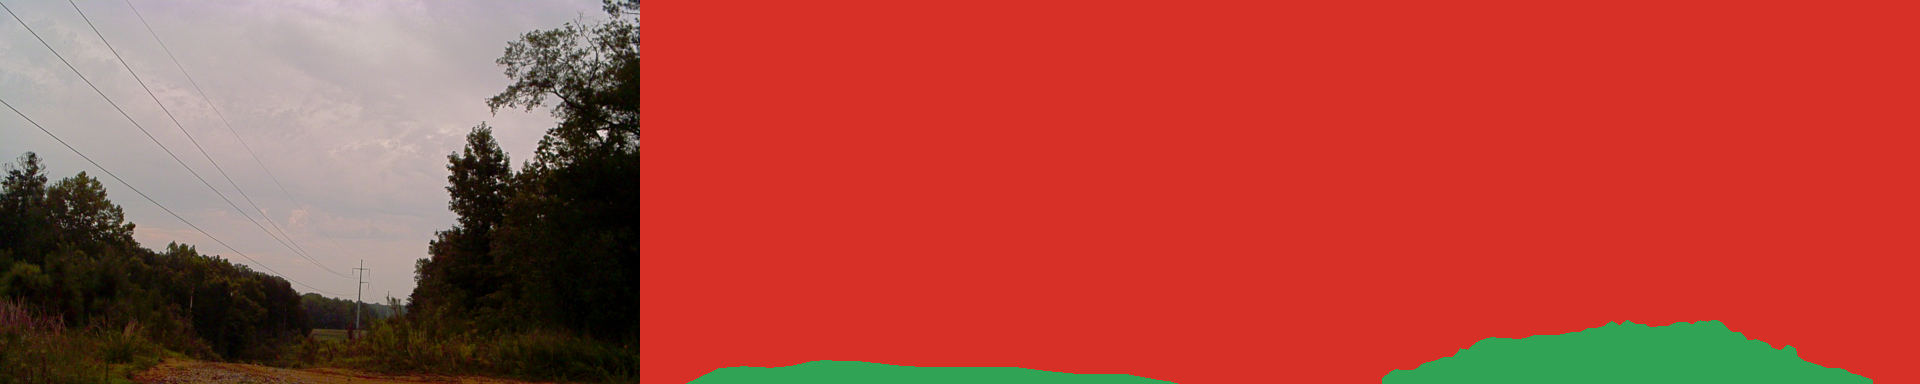
\includegraphics[width=0.96\linewidth]{figures/qualitative/pidnet_failure_boundary_mixed_459.png}
\caption[Asymmetric-error examples for reference PIDNet-S.]{Asymmetric-error
examples for reference PIDNet-S; each full-width triptych is RGB, ground truth, and
prediction. Top: \texttt{mixed\_pln\_1278}, maximum per-image FSR (30.20\%,
FBR 0.19\%). Middle: \texttt{mixed\_425}, maximum FBR (52.84\%, FSR 0.67\%).
Bottom: \texttt{mixed\_459}, 49.72\% boundary-band error (FSR 5.63\%, FBR
10.70\%).}
\label{fig:pidnet_failures}
\end{figure}

Figure~\ref{fig:pidnet_failures} provides the three ranked cases discussed
below: maximum FSR, maximum FBR, and severe boundary disagreement.

In the top case, the prediction opens almost the entire pale cultivated field
at the top and right of the image. The target admits the central and
foreground corridor but blocks that field under the blue+green policy. The
large connected green expansion explains the 30.20\% FSR; its spatial
coherence makes it more operationally important than the same number of
isolated pixels. The field and track share visual cues, so the example also
illustrates the annotation caveat: the model is clearly wrong relative to the
mask, but RGB alone does not reveal the physical property used to separate the
two capability regions.

In the middle case, the annotation marks a narrow path from the foreground
toward the left distance. The prediction retains only a small lower segment
and loses much of the shadowed corridor. This produces 52.84\% FBR but only
0.67\% FSR. It is conservative in the pixel convention, yet it could leave a
planner with no route. The weak distant contrast and narrow labelled geometry
connect the visible failure to the numerical rate.

The bottom case contains an irregular interface between low vegetation and
track. The prediction moves the foreground contour and changes the width of
the feasible strip. The global FSR and FBR are not as extreme, but nearly half
of the four-pixel-wide target boundary band is wrong. Because more than one
nearby contour can look plausible at this interface, the 49.72\% result should
be interpreted as precise disagreement with the supplied annotation, not as a
measurement of physical clearance error.

Together, the examples show three different remediation targets. False-safe
expansion suggests stronger physical cues, calibration, or planner-side
constraints. False blocks suggest better recall for narrow and shadowed
corridors. Boundary disagreement suggests boundary-aware supervision,
higher-quality annotation, or planning margins. A single loss change is
unlikely to address all three.

\section{Qualitative Transfer to ALICE}

\begin{figure}[H]
\centering
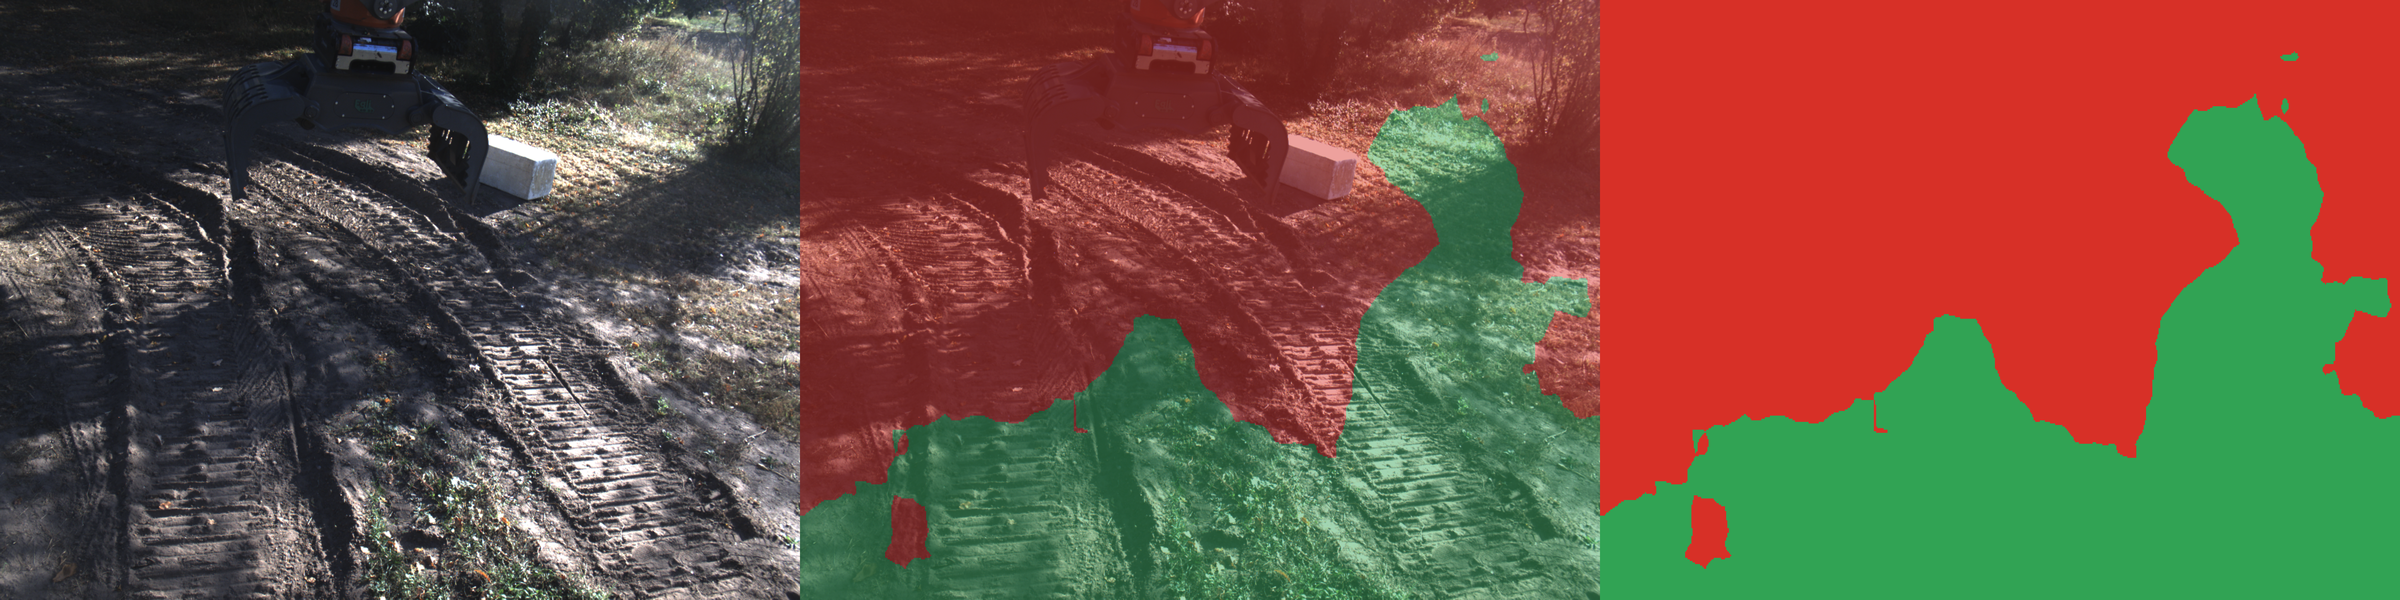
\includegraphics[width=0.96\linewidth]{figures/qualitative/pidnet_alice_sequence01.png}

\vspace{0.12cm}
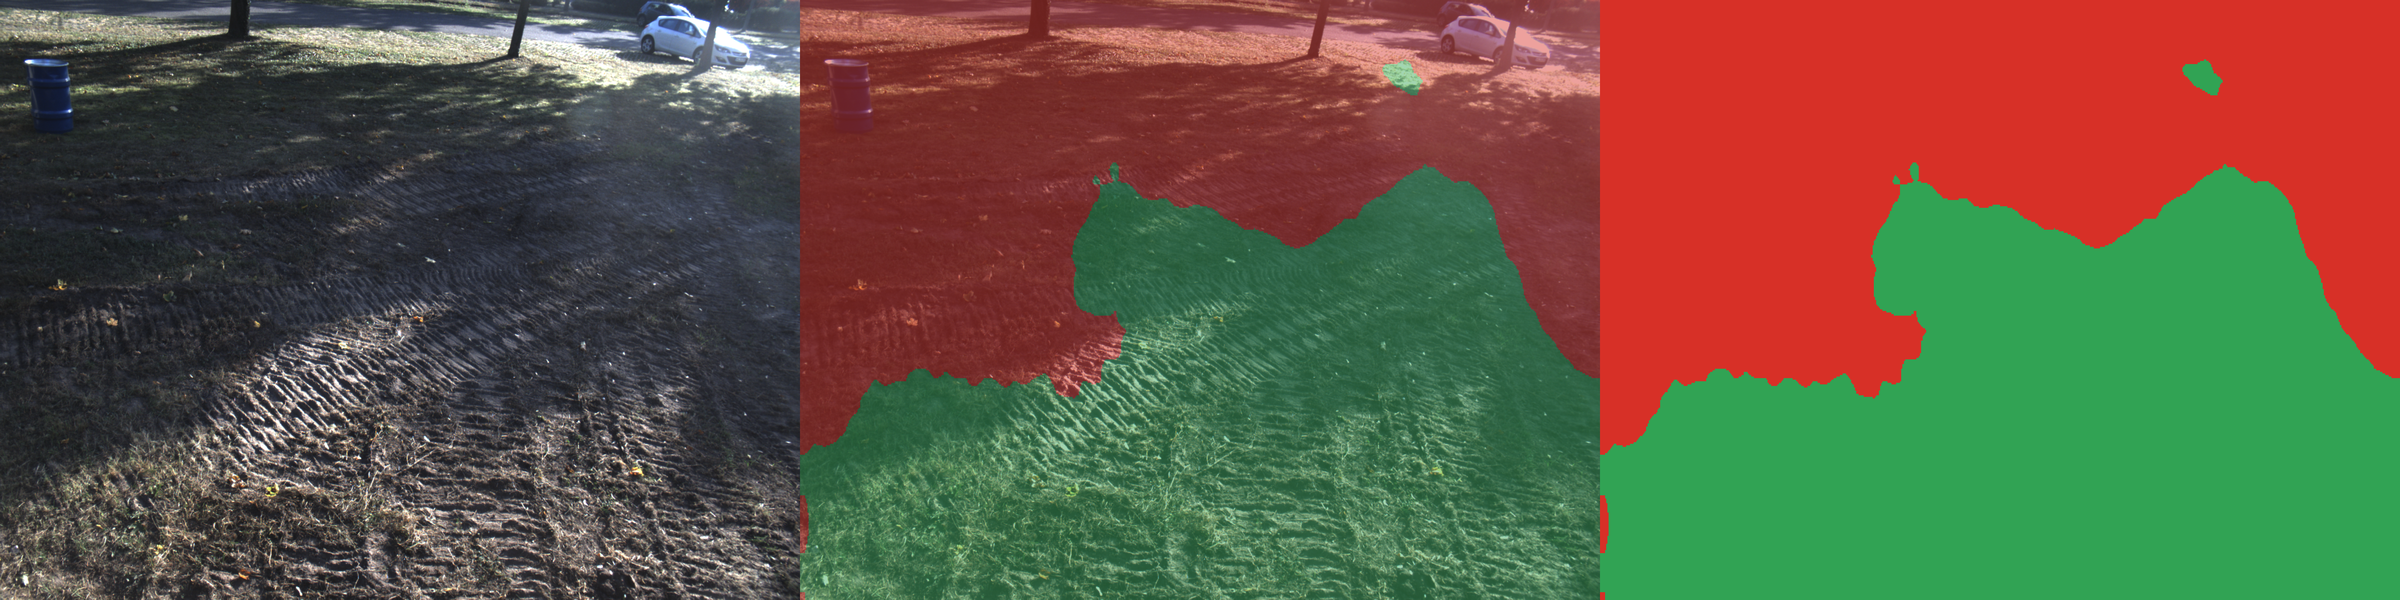
\includegraphics[width=0.96\linewidth]{figures/qualitative/pidnet_alice_sequence02.png}

\vspace{0.12cm}
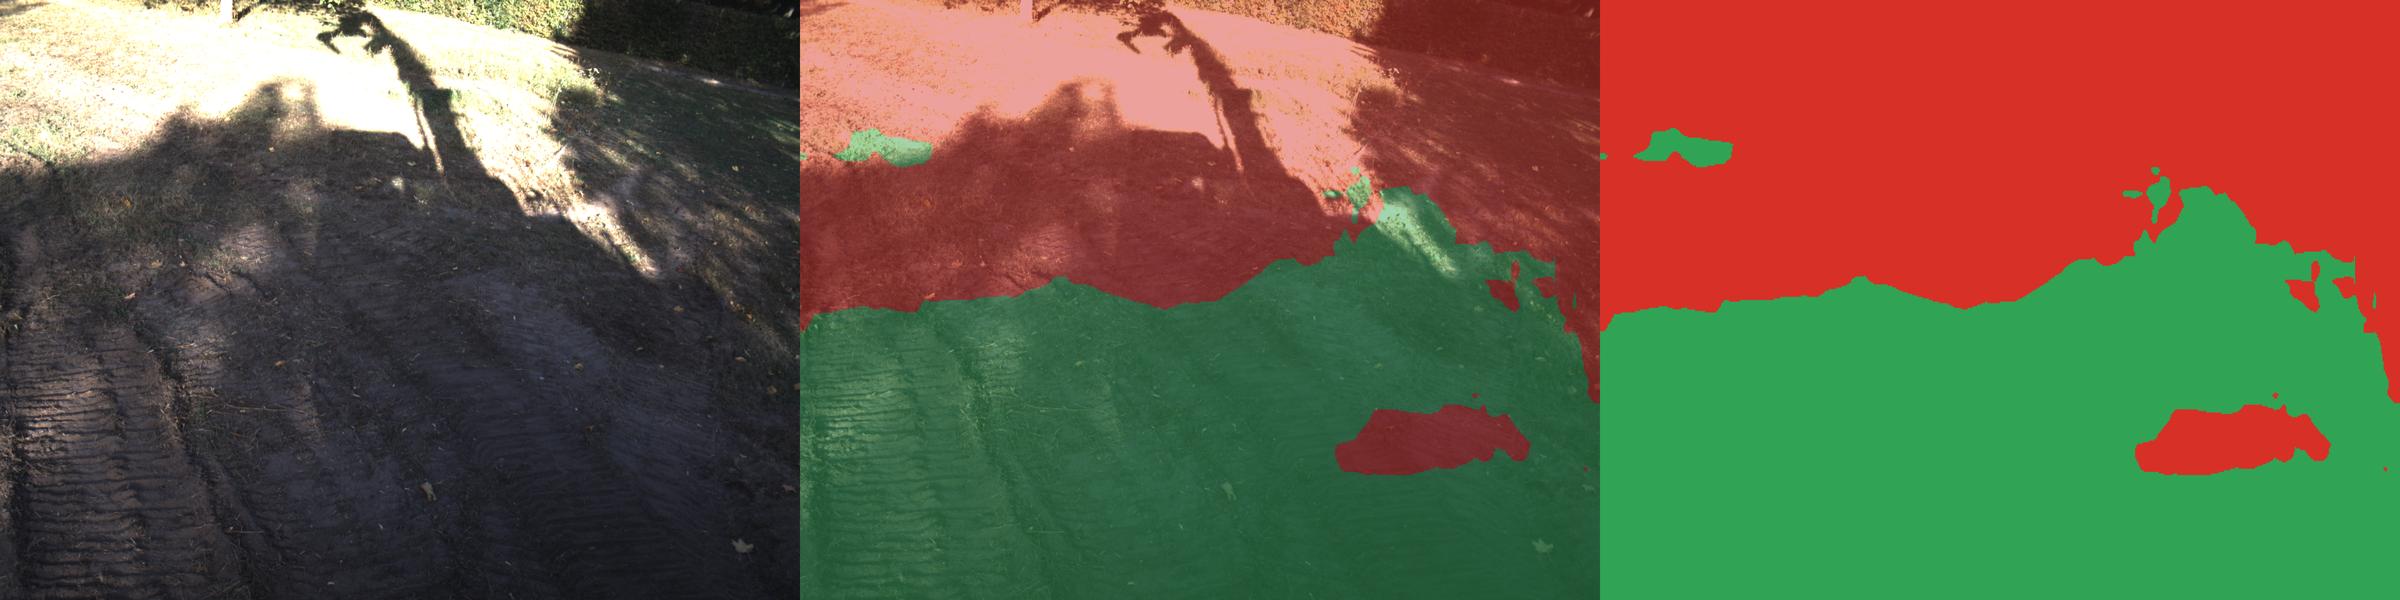
\includegraphics[width=0.96\linewidth]{figures/qualitative/pidnet_alice_sequence04.png}

\vspace{0.12cm}
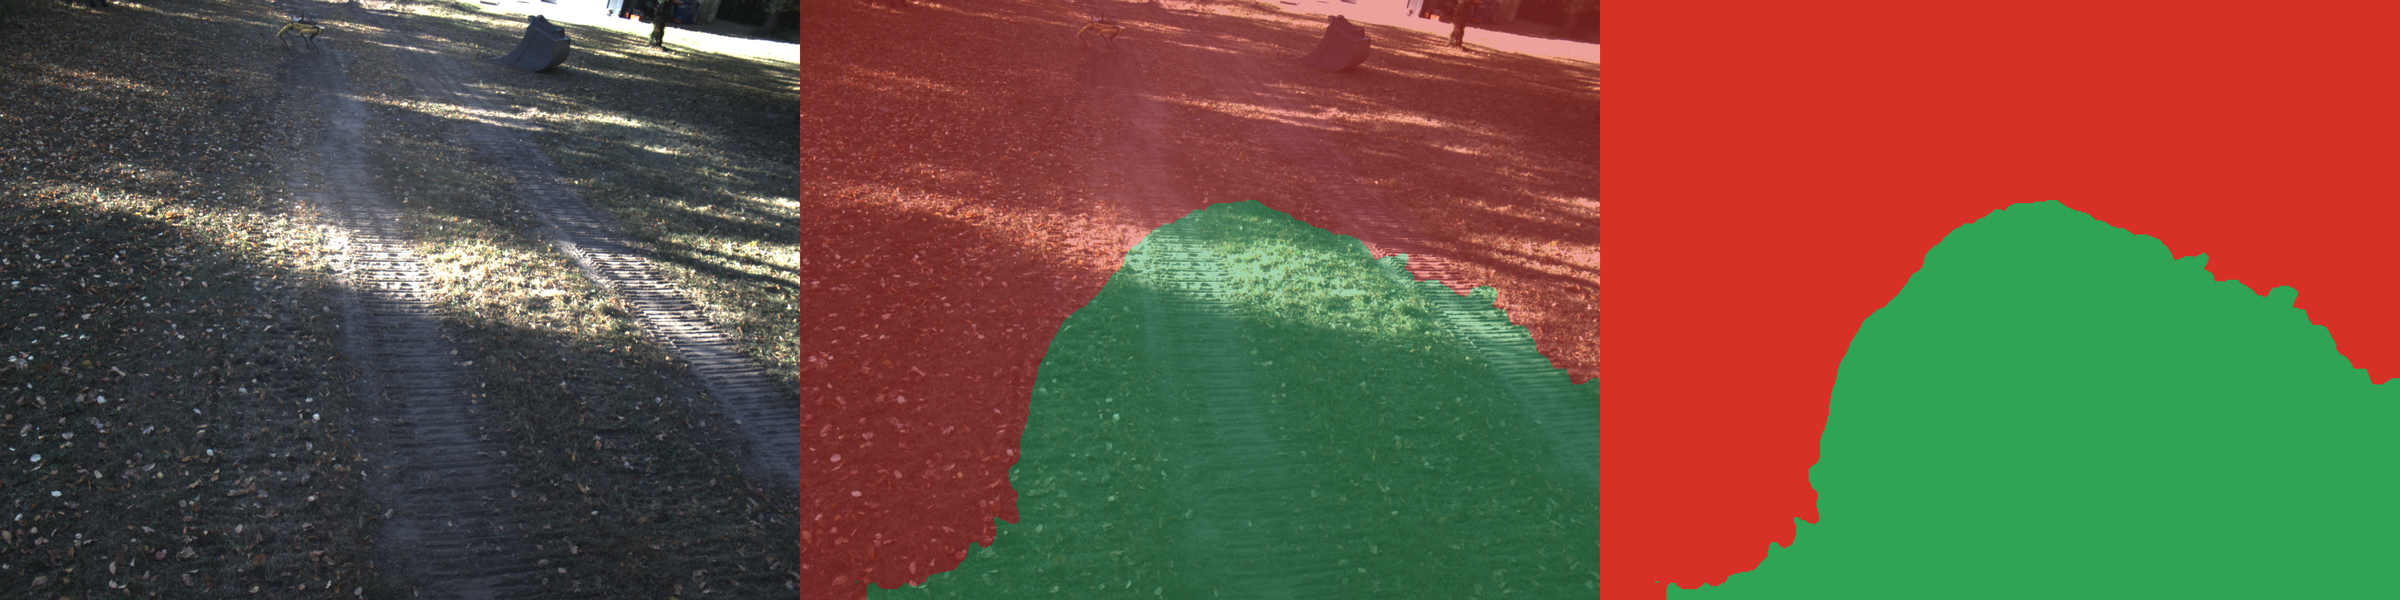
\includegraphics[width=0.96\linewidth]{figures/qualitative/pidnet_alice_sequence05.png}
\caption[Unscored PIDNet-S transfer to ALICE.]{Unscored transfer of the same
reference blue+green PIDNet-S checkpoint to the external ALICE mobile-robot
sequences. Each triptych shows RGB input, prediction overlay, and binary
prediction. No ALICE ground truth is available, so the panels show output
behaviour only.}
\label{fig:alice_transfer}
\end{figure}

Figure~\ref{fig:alice_transfer} is intentionally qualitative: it shows how the
fixed checkpoint responds to external scenes but supplies no accuracy claim.

The first ALICE frame contains another robot close to the camera. The model
mostly blocks the robot body and produces a narrow irregular traversable
region below and around it, showing that the output responds to a foreground
object rather than blindly opening the entire image. The second frame contains
grass, shadows, a paved road, a parked car, and a barrel. The prediction opens
a foreground grass wedge while largely blocking the road at the top. This is a
warning that a CaT-trained capability prior is not a general road detector.

The third frame has severe illumination contrast. The model forms a broad
foreground region but introduces holes and fragments near shadow boundaries.
The fourth frame contains a visible central worn track through leaf-covered
ground; the prediction forms a large connected lower region aligned only
partly with that visual track. Across the four scenes the masks are structured
and change with scene content, but their apparent plausibility varies.

No statement such as ``the model generalises to ALICE'' can be derived from
these images. There is no target mask, no vehicle trial, and no calibration
measurement. The panels only demonstrate that the reference pipeline executes on
the new camera data and reveal concrete behaviours that a future labelled
ALICE study should score.

% ============================================================
\chapter{Hardware and Inference-Speed Analysis}
\label{ch:hardware}
% ============================================================

\section{Why One FPS Number Is Insufficient}

Inference speed is a property of a complete execution configuration, not only
of a neural-network architecture. Processor, runtime, numerical precision,
batch size, tensor shape, compiler support, memory transfer, warm-up, and the
timer boundaries all affect the result. This chapter therefore keeps three
questions separate:
\begin{enumerate}
  \item how fast does the saved model execute on a consumer CPU?
  \item how do all nine architectures compare on one common server GPU?
  \item what throughput is obtained after compiling the two deployed
  checkpoints into fixed TensorRT engines and including preprocessing and mask
  return?
\end{enumerate}

No speed value is borrowed from an architecture paper for ranking. Published
Cityscapes or A6000 FPS figures use a different image size, model output, runtime, and
hardware. Every table below names its own scope.

\section{Ryzen 5 5500 CPU Results}

Table~\ref{tab:cpu_comparison} reports batch-one forward throughput with six
PyTorch threads. Eager PIDNet-S reaches 21.16 FPS with 47.25 ms mean latency
for the reference checkpoint. Its median is 46.45 ms and P95 is 55.63 ms.
This confirms GPU-free operation at a modest perception rate, but the timer
does not include camera decode or planning.

\begin{table}[H]
\centering
\caption{Ryzen~5~5500 batch-one throughput at $640\times384$. Values are
forward and prediction only; compiled timing excludes compilation warm-up.}
\label{tab:cpu_comparison}
\small
\begin{tabular}{@{}lrrr@{}}
\toprule
\textbf{Model} & \textbf{Eager FPS} & \textbf{Compiled FPS} & \textbf{Compiled mean latency} \\
\midrule
DDRNet-23-Slim & 27.74 & \textbf{36.50} & 27.40 ms \\
PIDNet-S & 21.16 & 27.04 & 36.98 ms \\
BiSeNetV2 & 11.48 & 16.34 & 61.20 ms \\
FPN/MobileNetV2 & 7.23 & 14.26 & 70.13 ms \\
FPN/EfficientNet-B0 & 5.92 & 11.70 & 85.47 ms \\
U-Net/MobileNetV2 & 7.10 & 10.15 & 98.52 ms \\
U-Net/EfficientNet-B0 & 6.96 & 9.66 & 103.52 ms \\
SegFormer-B0 & 4.38 & 8.23 & 121.51 ms \\
ROD ViT-S & 0.41 & 0.46 & 2,195.96 ms \\
\bottomrule
\end{tabular}
\end{table}

Compiled DDRNet-23-Slim is the CPU throughput leader at 36.50 FPS. Its
convergence-aware blue+green mIoU, however, is the lowest in the nine-model
table at 0.9095. PIDNet-S is slower but reaches 0.9195.
FPN/EfficientNet-B0 reaches only 11.70 compiled FPS but gives the highest mean
accuracy, 0.9423. The CPU therefore presents a clear sequence of trade-offs
rather than one winner. ROD reaches 0.41 eager FPS and 0.46 compiled FPS; its
frozen encoder reduces training-time optimisation but the full internally
resized $1024\times1024$ transformer remains active during inference.

Compiler benefit is architecture-dependent. FPN/MobileNetV2 nearly doubles its
throughput, and SegFormer-B0 improves substantially, while U-Net and PIDNet
receive smaller gains. These differences show why floating-point-operation
(FLOP) counts or parameter estimates cannot substitute for runtime
measurements. Compilation raises ROD throughput by only 11.2\%, from 0.4094 to
0.4554 FPS, leaving the current implementation unsuitable for CPU-rate
perception loops.

\section{Common H100 Results}

The H100 protocol controls hardware and eager FP32 execution across all nine
systems. PIDNet-S is fastest at 270.38 FPS. DDRNet-23-Slim follows at 245.17
FPS, while ROD is slowest at 21.79 FPS. The frozen encoder reduces ROD training
gradients but does not reduce inference work; the full transformer remains on
the forward path.

\begin{table}[H]
\centering
\caption{Parameter count and common H100 NVL 3g.47GB MIG batch-one
forward throughput. External input is $640\times384$; execution is eager FP32.}
\label{tab:h100_comparison}
\small
\begin{tabular}{@{}lrrr@{}}
\toprule
\textbf{Model} & \textbf{Parameters} & \textbf{Mean FPS} & \textbf{Mean latency} \\
\midrule
PIDNet-S & 7.62 M & \textbf{270.38} & 3.70 ms \\
DDRNet-23-Slim & 5.69 M & 245.17 & 4.08 ms \\
BiSeNetV2 & 3.34 M & 167.80 & 5.96 ms \\
FPN/MobileNetV2 & 4.22 M & 147.36 & 6.79 ms \\
SegFormer-B0 & 3.71 M & 141.23 & 7.08 ms \\
U-Net/MobileNetV2 & 6.63 M & 131.86 & 7.58 ms \\
FPN/EfficientNet-B0 & 5.76 M & 131.40 & 7.61 ms \\
U-Net/EfficientNet-B0 & 6.25 M & 101.24 & 9.88 ms \\
ROD ViT-S & 29.11 M & 21.79 & 45.89 ms \\
\bottomrule
\end{tabular}
\end{table}

Table~\ref{tab:h100_comparison} reports the measured H100 throughput and
latency for every architecture under this common scope.

On the same H100 protocol, PIDNet-S is approximately 12.4 times faster than
ROD. Under convergence-aware training, ROD's blue+green mean is 1.36 points
higher, so that accuracy improvement has a large latency price. In the
nine-model table, ROD is also slower
and less accurate than FPN/EfficientNet-B0 on this particular hardware and
recipe. This does not make ROD universally inferior: a model-specific compiler,
different training objective, memory constraint, or another dataset can change
the decision. It does mean that the controlled H100 evidence does not place
ROD on the observed accuracy--speed frontier.

Parameter count again fails to determine speed. SegFormer-B0 has only 3.71
million parameters but is much slower than PIDNet-S on CPU. BiSeNetV2 is the
smallest system but not the fastest H100 model. Operator mix, feature-map size,
attention, memory traffic, and kernel implementation matter alongside stored
weights.

\section{Accuracy--Speed Relationship}

Figure~\ref{fig:accuracy_speed_h100} combines convergence-aware blue+green mean
mIoU with the existing H100 throughput measurements. Moving upward improves
accuracy; moving right improves speed. No model occupies the upper-right
corner.

\begin{figure}[H]
\centering
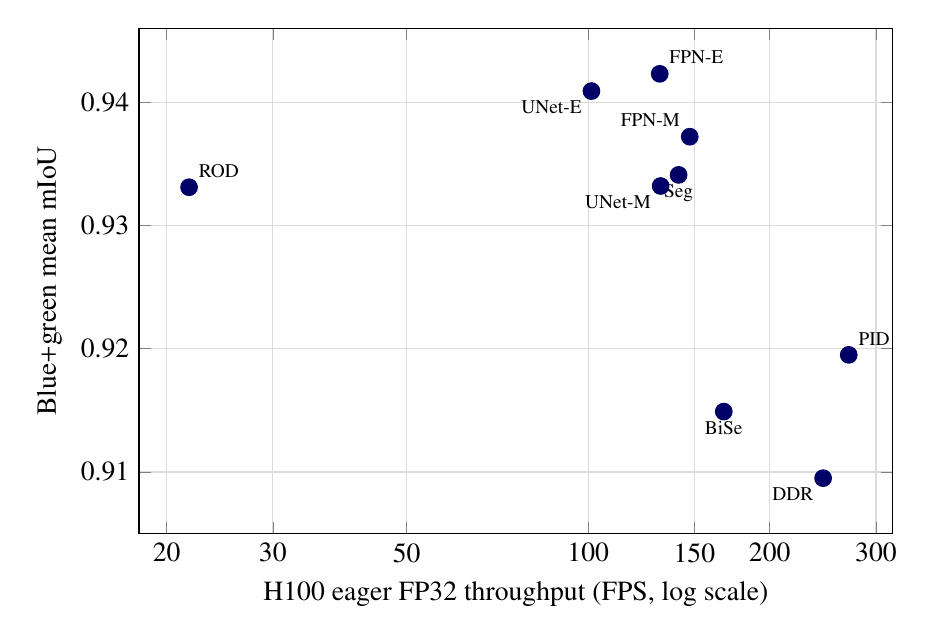
\begin{tikzpicture}
\begin{axis}[
  width=0.92\textwidth,
  height=8.0cm,
  xmode=log,
  xmin=18,xmax=320,
  ymin=0.905,ymax=0.946,
  xlabel={H100 eager FP32 throughput (FPS, log scale)},
  ylabel={Blue+green mean mIoU},
  grid=both,
  grid style={line},
  xtick={20,30,50,100,150,200,300},
  xticklabels={20,30,50,100,150,200,300}
]
\addplot[only marks,mark=*,mark size=3pt,color=azulUC3M] coordinates {
  (270.38,0.9195)
  (245.17,0.9095)
  (167.80,0.9149)
  (147.36,0.9372)
  (141.23,0.9341)
  (131.86,0.9332)
  (131.40,0.9423)
  (101.24,0.9409)
  (21.79,0.9331)
};
\node[font=\scriptsize,anchor=south west] at (axis cs:270.38,0.9195) {PID};
\node[font=\scriptsize,anchor=north east] at (axis cs:245.17,0.9095) {DDR};
\node[font=\scriptsize,anchor=north] at (axis cs:167.80,0.9149) {BiSe};
\node[font=\scriptsize,anchor=south east] at (axis cs:147.36,0.9372) {FPN-M};
\node[font=\scriptsize,anchor=north] at (axis cs:141.23,0.9341) {Seg};
\node[font=\scriptsize,anchor=north east] at (axis cs:131.86,0.9332) {UNet-M};
\node[font=\scriptsize,anchor=south west] at (axis cs:131.40,0.9423) {FPN-E};
\node[font=\scriptsize,anchor=north east] at (axis cs:101.24,0.9409) {UNet-E};
\node[font=\scriptsize,anchor=south west] at (axis cs:21.79,0.9331) {ROD};
\end{axis}
\end{tikzpicture}
\caption[Blue+green accuracy versus H100 throughput.]{Blue+green mean mIoU
versus common H100 throughput. E and M denote EfficientNet-B0 and
MobileNetV2. FPN/EfficientNet-B0 supplies the highest accuracy, while PIDNet-S
provides the highest throughput. Accuracy uses the convergence-aware
blue+green suite; inference speed uses the unchanged architecture graphs.}
\label{fig:accuracy_speed_h100}
\end{figure}

For a latency-first H100 deployment, PIDNet-S offers the most headroom. The FPN
with MobileNetV2 adds 1.77 mIoU points while retaining 147.36 FPS. Replacing
that encoder with EfficientNet-B0 adds another 0.50 points at 131.40 FPS and
gives the highest observed accuracy mean. The EfficientNet-B0 U-Net is 0.13
points lower and also has lower throughput in this runtime. The plotted means
do not include latency variance or model-specific compiler tuning, so the
frontier is specific to the declared protocol.

The CPU frontier differs. Compiled DDRNet supplies the only measured rate above
30 FPS, PIDNet-S offers a stronger accuracy point at 27.04 FPS, and
FPN/EfficientNet-B0 provides the highest accuracy at 11.70 FPS. A robot with a
10 Hz perception requirement may select a different model from one requiring
30 Hz. Frame rate should therefore be treated as a constraint in the model
choice, not as an isolated leaderboard.

\section{RTX 5060 TensorRT Results}

TensorRT changes the deployment picture for the two exported checkpoints.
Table~\ref{tab:tensorrt_speed} reports both device and measured-pipeline
scopes. PIDNet-S reaches 106.43 pipeline FPS with 9.396 ms mean latency. ROD
reaches 39.38 pipeline FPS with 25.392 ms mean latency. ROD therefore crosses
a nominal 30 FPS threshold for the measured pipeline after compilation,
although the unmeasured camera and planning stages still consume part of a
real 33.3 ms frame budget.

\begin{table}[H]
\centering
\caption[TensorRT batch-one timing on the RTX 5060.]{FP16-enabled
mixed-precision TensorRT batch-one timing on the
RTX~5060. Each distribution contains 320 measured samples after warm-up.}
\label{tab:tensorrt_speed}
\small
\begin{tabular}{@{}llrrrr@{}}
\toprule
\textbf{Model} & \textbf{Scope} & \textbf{Mean} & \textbf{P50} & \textbf{P95} & \textbf{FPS} \\
\midrule
\multirow{2}{*}{PIDNet-S}
 & Device & 0.963 ms & 0.880 ms & 1.414 ms & 1,037.97 \\
 & Measured pipeline & 9.396 ms & 9.178 ms & 10.943 ms & \textbf{106.43} \\
\midrule
\multirow{2}{*}{ROD ViT-S}
 & Device & 17.401 ms & 17.397 ms & 17.669 ms & 57.47 \\
 & Measured pipeline & 25.392 ms & 25.255 ms & 26.580 ms & \textbf{39.38} \\
\bottomrule
\end{tabular}
\end{table}

Figure~\ref{fig:tensorrt_frame_budget} expresses the same result as a frame
budget. At 30 FPS, one complete cycle may occupy at most 33.33 ms. The coloured
segment is the measured TensorRT pipeline; the pale segment is only remaining
time, not a measurement of the omitted camera, transport, planning, and control
stages.

\begin{figure}[H]
\centering
\resizebox{0.92\textwidth}{!}{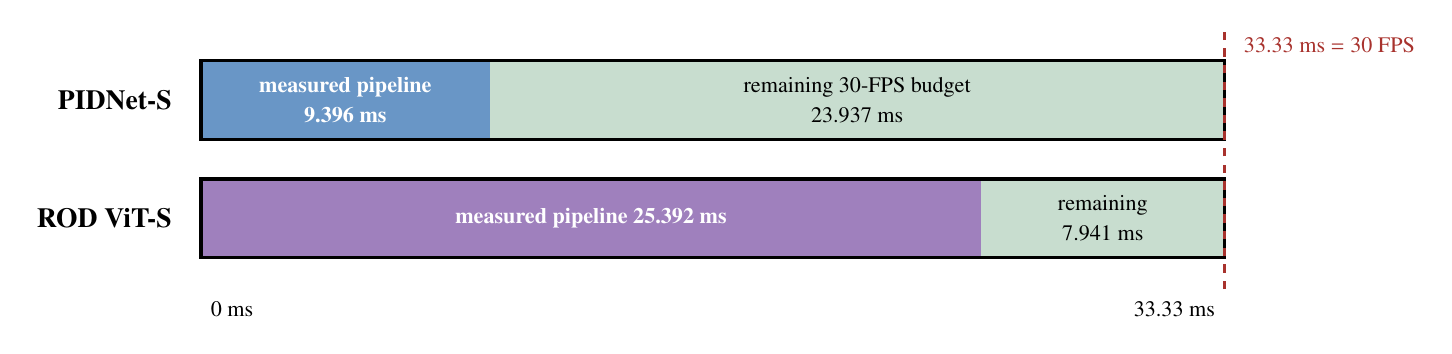
\begin{tikzpicture}[font=\sffamily\small]
  \def\scale{0.39}
  \def\budget{13.0}
  \def\pid{3.664}
  \def\rod{9.903}

  \node[anchor=east,font=\bfseries] at (-0.25,2.35) {PIDNet-S};
  \node[anchor=east,font=\bfseries] at (-0.25,0.85) {ROD ViT-S};

  \fill[pidP!72] (0,1.85) rectangle (\pid,2.85);
  \fill[good!26] (\pid,1.85) rectangle (\budget,2.85);
  \draw[very thick] (0,1.85) rectangle (\budget,2.85);
  \node[text=white,font=\bfseries\footnotesize,align=center] at ({\pid/2},2.35)
    {measured pipeline\\9.396 ms};
  \node[font=\footnotesize,align=center] at ({(\pid+\budget)/2},2.35)
    {remaining 30-FPS budget\\23.937 ms};

  \fill[pidD!72] (0,0.35) rectangle (\rod,1.35);
  \fill[good!26] (\rod,0.35) rectangle (\budget,1.35);
  \draw[very thick] (0,0.35) rectangle (\budget,1.35);
  \node[text=white,font=\bfseries\footnotesize,align=center] at ({\rod/2},0.85)
    {measured pipeline 25.392 ms};
  \node[font=\footnotesize,align=center] at ({(\rod+\budget)/2},0.85)
    {remaining\\7.941 ms};

  \draw[safety,very thick,dashed] (\budget,-0.05) -- (\budget,3.25);
  \node[anchor=west,font=\footnotesize,text=safety] at (\budget+0.12,3.05)
    {33.33 ms = 30 FPS};
  \node[anchor=west,font=\footnotesize] at (0,-0.30) {0 ms};
  \node[anchor=east,font=\footnotesize] at (\budget,-0.30) {33.33 ms};
\end{tikzpicture}
}
\caption[TensorRT latency within a 30-FPS frame budget.]{Measured RTX~5060
TensorRT pipeline latency within a nominal 30-FPS frame budget. PIDNet-S leaves
substantially more unallocated time than ROD, but neither bar measures the
remaining robot stack. Original graphic drawn from the results in
Table~\ref{tab:tensorrt_speed}.}
\label{fig:tensorrt_frame_budget}
\end{figure}

The gap between PIDNet's 0.963 ms device time and 9.396 ms pipeline time shows
that host preprocessing and transfers dominate after the small network is
compiled. ROD still spends most of its time in the engine, because the internal
$1024\times1024$ transformer remains expensive. Improving CPU resize or transfer would
therefore benefit PIDNet proportionally more than ROD.

The TensorRT values should not be interpreted as a controlled speed-up over
the H100 or Ryzen tables because the GPU, runtime, and precision all change.
They answer a deployment question: what rate do the saved checkpoints achieve
after hardware-specific compilation on the available local GPU?

\section{Mixed-Precision Accuracy Verification}

Full-test evaluation confirms that mixed-precision conversion does not materially change
the operating points. Table~\ref{tab:tensorrt_accuracy} compares each engine
with its source PyTorch checkpoint.

\begin{table}[H]
\centering
\caption{Full 544-image comparison of each source PyTorch checkpoint with its
mixed-precision TensorRT conversion.}
\label{tab:tensorrt_accuracy}
\small
\begin{tabular}{@{}lrrrr@{}}
\toprule
\textbf{Model/runtime} & \textbf{mIoU} & \textbf{FSR} & \textbf{FBR} & \textbf{mIoU change} \\
\midrule
PIDNet-S PyTorch & 0.893941 & 4.3176\% & 7.0369\% & reference \\
PIDNet-S TensorRT & 0.893764 & 4.3117\% & 7.0667\% & $-0.000177$ \\
\midrule
ROD PyTorch paper recipe & 0.923569 & 3.85\% & 3.97\% & reference \\
ROD TensorRT & 0.923635 & 3.8508\% & 3.9574\% & $+0.000066$ \\
\bottomrule
\end{tabular}
\end{table}

PIDNet changes by 0.0177 mIoU percentage points and ROD by 0.0066 points.
Small positive or negative differences are expected when probabilities close
to 0.50 cross the threshold after mixed-precision execution. The full confusion
matrices, rather than a small image sample, support the claim that both
conversions preserve accuracy at the precision used for architectural
interpretation.

\section{Deployment Meaning}

Three distinct deployment candidates emerge:
\begin{itemize}
  \item \textbf{CPU-constrained:} compiled DDRNet maximises frame rate, while
  PIDNet-S offers a more accurate near-real-time alternative. The
  EfficientNet systems require a lower frame-rate budget, and the current ROD
  implementation is not a practical CPU candidate.
  \item \textbf{Powerful common GPU:} PIDNet-S maximises throughput;
  FPN/EfficientNet-B0 provides the highest accuracy above 100 FPS on the H100
  protocol, followed by U-Net/EfficientNet-B0.
  \item \textbf{Available RTX TensorRT path:} the reference PIDNet model
  exceeds 100 pipeline FPS, while the more accurate reconstructed ROD model
  reaches 39.4 FPS.
\end{itemize}

None of these measurements includes sensor exposure, decode, inter-process
transport, projection into vehicle coordinates, temporal filtering, path
planning, or control. Power draw, thermal throttling, and embedded-GPU
behaviour are also unmeasured. The results establish inference capacity and an
accuracy--latency trade-off, not production readiness of a complete autonomous
system.

% ============================================================
\chapter{Discussion and Research Outlook}
\label{ch:discussion}
% ============================================================

\section{Synthesis of Findings}

The PIDNet-S experiments establish that the CaT capability labels can be
learned by a compact network at useful accuracy and latency. The retained
7.62-million-parameter model reaches 0.893941 mIoU, and an independent CPU run
reconstructs its complete confusion matrix exactly. This level of
reproducibility connects the reported rates to one identifiable model rather
than to an undocumented training run. It remains a CaT result, however;
neither the exact score nor its operational interpretation transfers automatically
to another site or vehicle.

Several seemingly reasonable interventions did not work as intended. The
tested photometric augmentation reduced performance, the additional
false-safe term increased both asymmetric error rates, and greater input
resolution provided no benefit while halving the batch size. Neutral class
weights recovered more traversable pixels but did not give the strongest
combined operating point. By contrast, threshold adjustment behaved
predictably: it traded false-safe openings for false blocks without eliminating
the underlying errors. These outcomes argue for controlled measurements of
engineering choices rather than assumptions based on their names or intent.

Pretrained feature transfer changes the attainable accuracy, but training
horizon changes the comparison as well. Under the original matched 15-epoch
conditions, ROD improves mean mIoU over PIDNet-S by 3.15 percentage points for
blue+green and 3.79 points for blue-only. The convergence-aware blue+green
follow-up raises both means to 0.9331 and 0.9195, narrowing their difference to
1.36 points. Across all nine systems, FPN/EfficientNet-B0 reaches
$0.9423\pm0.0005$ and is highest in each of the three executed seeds;
U-Net/EfficientNet-B0 follows at $0.9409\pm0.0004$. ROD remains below the five
pretrained encoder--decoder alternatives but nearly matches
U-Net/MobileNetV2. These changes show that the earlier matrix described
performance after equal early exposure, not a converged architecture ranking.

Runtime supplies a different ordering. PIDNet-S produces the highest H100
throughput, compiled DDRNet-23-Slim leads on the tested CPU, and the two
EfficientNet-B0 systems provide the greatest overlap. TensorRT brings the
reconstructed ROD model to 39.38 FPS for the measured local pipeline, but
PIDNet-S remains much faster at 106.43 FPS. On the Ryzen CPU, ROD reaches only
0.41 eager FPS and 0.46 compiled FPS because freezing removes encoder gradients
during training but not encoder computation during inference. Model selection
is consequently a constraint problem involving target frame rate, runtime, and
acceptable error profile, not a lookup of the largest mIoU.

\section{Interpreting the Architecture Results}

The comparison does not support a simple narrative that transformers are more
accurate and CNNs are faster. ROD's pretrained transformer improves over
randomly initialised PIDNet-S, but FPN and U-Net with a compact pretrained
convolutional EfficientNet-B0 encoder perform better under the common recipe.
SegFormer-B0 lies between the EfficientNet and MobileNet systems. The best
observed result is therefore associated with strong pretrained compact
features and an effective multiscale decoder, not with one architecture
category alone.

The $2\times2$ subset suggests that encoder choice has the larger effect:
EfficientNet-B0 improves both decoders, while FPN's advantage over U-Net is
0.13 points with EfficientNet and 0.41 points with MobileNetV2. FPN is higher
for every matched encoder--seed pair in the convergence suite. With only two
encoders and two decoders, this remains a local interaction, not a universal
conclusion about FPN or U-Net.

ROD's reconstructed training result shows that optimisation is
architecture-dependent. CE alone, neutral weights, a larger learning rate, and
polynomial decay improve ROD relative to the common CE+Dice recipe. This does
not invalidate the retained PIDNet configuration. It shows that a recipe
selected during one architecture's development should not be assumed optimal
for another.

The real-time architectures occupy different parts of the speed--accuracy
plane. DDRNet provides the highest compiled CPU rate but the lowest
convergence-aware blue+green accuracy. PIDNet provides the highest H100
throughput, a verified deployment chain, and now a higher mean mIoU than
BiSeNetV2. The phrase ``real-time architecture'' therefore describes design
intent, not a fixed ranking on every processor.

\section{Meaning of the Asymmetric Error Metrics}

The reference PIDNet model has lower FSR than FBR, which indicates a conservative
aggregate operating balance. The maximum-FSR image demonstrates why that
statement is insufficient: a 4.32\% global rate can coexist with a 30.20\%
per-image rate and one connected expansion into a large field. Conversely, the
maximum-FBR example shows a visually coherent route being almost removed.

The highest-scoring models reduce both directions, so their accuracy gain is not
obtained simply by opening or closing the entire mask. Even then, pixel rates
do not specify whether an error intersects the planned trajectory. A false-safe
pixel behind the vehicle and one under the projected front wheel contribute
equally. Connectedness, distance, obstacle type, speed, and confidence are
absent.

The metrics are best used as three layers of evidence:
\begin{enumerate}
  \item mIoU and class IoU summarise balanced segmentation overlap;
  \item FSR and FBR expose the direction of disagreement;
  \item ranked visual review shows the spatial form of the error.
\end{enumerate}

Figure~\ref{fig:safety_evidence_ladder} shows why these layers should not be
collapsed into a single safety claim. This thesis evaluates pixel disagreement
and its spatial form. Whether an error changes a route, and whether the vehicle
then collides or loses progress, require a planner and physical system that are
outside the present experiment.

\begin{figure}[H]
\centering
\resizebox{\textwidth}{!}{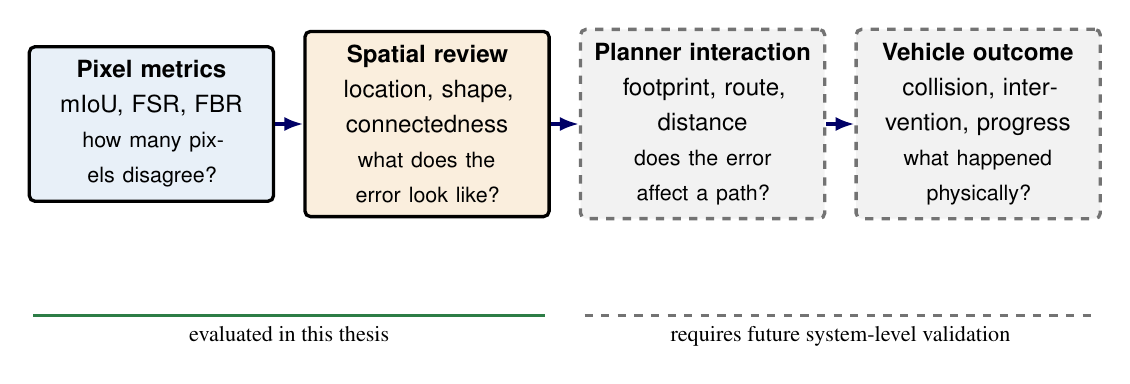
\begin{tikzpicture}[
  font=\sffamily\small,
  stage/.style={draw,rounded corners=2pt,very thick,align=center,
    text width=2.75cm,minimum height=1.95cm,inner sep=5pt},
  future/.style={stage,dashed,draw=black!55,fill=black!5},
  flow/.style={-{Latex[length=2.4mm]},very thick,draw=azulUC3M}
]
  \node[stage,fill=softblue] (metrics) at (1.55,2.05)
    {\textbf{Pixel metrics}\\mIoU, FSR, FBR\\\footnotesize how many pixels disagree?};
  \node[stage,fill=softorange] (spatial) at (5.05,2.05)
    {\textbf{Spatial review}\\location, shape, connectedness\\\footnotesize what does the error look like?};
  \node[future] (planner) at (8.55,2.05)
    {\textbf{Planner interaction}\\footprint, route, distance\\\footnotesize does the error affect a path?};
  \node[future] (vehicle) at (12.05,2.05)
    {\textbf{Vehicle outcome}\\collision, intervention, progress\\\footnotesize what happened physically?};
  \draw[flow] (metrics) -- (spatial);
  \draw[flow] (spatial) -- (planner);
  \draw[flow] (planner) -- (vehicle);

  \draw[very thick,good] (0.05,-0.38) -- node[below,font=\footnotesize,text=black]
    {evaluated in this thesis} (6.55,-0.38);
  \draw[very thick,dashed,black!55] (7.05,-0.38) -- node[below,font=\footnotesize,text=black]
    {requires future system-level validation} (13.55,-0.38);
\end{tikzpicture}
}
\caption[From pixel metrics to vehicle-level evidence.]{Evidence required to
move from segmentation quality to a vehicle-level safety statement. Solid
stages are evaluated here; dashed stages require future planner and vehicle
experiments. Original schematic drawn for this thesis.}
\label{fig:safety_evidence_ladder}
\end{figure}

A later planner-level study should add collision, intervention, route
availability, progress, and time-to-goal measures rather than attempting to
turn FSR alone into a safety certificate.

\section{Annotation and Task Uncertainty}

CaT's vehicle-capability concept is a strength because it is closer to
navigation than a material label. It also introduces judgement. A sharp
semantic boundary between a track and adjacent vegetation may be visible in
RGB; the exact boundary between pickup-traversable and off-road-only soil may
depend on slope, compaction, moisture, hidden roughness, or an annotator's
vehicle model.

The selected examples make this limitation concrete without declaring the
reference wrong. In \texttt{mixed\_pln\_1278}, a pale field and the accepted
track look similar. In \texttt{mixed\_118}, dense woodland and leaf-covered
ground provide little visible support for the broad accepted foreground
region. In \texttt{mixed\_459}, several nearby vegetation--track contours
appear visually possible. The masks may encode knowledge unavailable
in the RGB frame, and visual ambiguity does not imply that both regions would
support a vehicle equally.

Because the dataset provides one released annotation per image and no
inter-annotator agreement, the thesis cannot estimate label variance, separate
model error from annotation uncertainty, or provide an upper bound on
RGB-only performance. A model that reproduces the labels perfectly would
reproduce their assumptions; it would not necessarily predict vehicle outcome
perfectly.

\section{Limitations}

\begin{enumerate}
  \item \textbf{One small, imbalanced dataset.} Training uses 1,002 images from
  three environments, with Power Line dominating. No environment-stratified
  result or geographically independent dataset is reported.

  \item \textbf{Sample-level split.} The deterministic hash prevents direct
  identifier overlap, but it does not explicitly group visually adjacent or
  near-duplicate frames. The degree of correlation between training and
  validation samples is not measured.

  \item \textbf{Annotation uncertainty is unquantified.} There are no repeated
  labels, annotator confidence scores, vehicle trials, or agreement statistics.

  \item \textbf{RGB cannot observe every physical constraint.} Support,
  deformability, water depth, slope, clearance, and wheel slip may require
  geometry, temporal evidence, or interaction.

  \item \textbf{Policy dependence.} Blue-only and blue+green are explicit
  vehicle policies. Results do not transfer numerically to blue+green+red,
  four-class CaT, or a different vehicle.

  \item \textbf{Repeated benchmark use.} Test images are excluded from
  optimisation and automatic checkpoint selection, but the project reports
  many test runs. The benchmark is not a single-use blinded evaluation.

  \item \textbf{Limited statistical scope.} The controlled ablation has one
  seed. The architecture table has three selected seeds on one fixed split and uses
  population standard deviation, not confidence intervals or hypothesis tests.

  \item \textbf{Architecture and pretraining are confounded.} PIDNet-S and
  DDRNet start randomly, while the leading systems use pretrained encoders.
  The table ranks complete recipes and cannot isolate causal architecture
  effects.

  \item \textbf{The convergence rule is shared, not model-specific
  optimisation.} The follow-up removes the obviously early 15-epoch stopping
  point for blue+green, but all models still share one objective, learning-rate
  schedule, and patience rule. Individually tuned recipes could change the
  ranking, and the blue-only matrix remains a fixed-budget result.

  \item \textbf{Two training software environments were used.} The FPN,
  U-Net, and SegFormer runs used PyTorch 2.13.0/CUDA 13.0; PIDNet, ROD,
  DDRNet, and BiSeNet used PyTorch 2.7.1/CUDA 12.6. The data, configuration,
  hardware partition, and evaluator were fixed, but framework version remains
  a cross-family confound.

  \item \textbf{Checkpoint availability differs from checkpoint identity.}
  The convergence suite records server-side SHA-256 identities for all 27
  selected checkpoints, but their binaries are not present locally. The
  reference PIDNet checkpoint remains the fully local reproduction chain.

  \item \textbf{Convergence training time is not usable evidence.} Shared-GPU
  workers were paused and resumed to control contention. This preserves
  training state but makes their recorded wall-clock duration unsuitable for
  comparing training cost.

  \item \textbf{Qualitative comparison is centred on PIDNet.} The detailed
  percentile, failure, and ALICE panels use the reference PIDNet model.
  Equivalent ROD and top-FPN failure panels were not produced, so qualitative
  error differences between architectures are not established.

  \item \textbf{ALICE is unlabelled.} The model output can be inspected, but no
  cross-domain accuracy or error rate can be calculated.

  \item \textbf{Pixel metrics omit planning and time.} No temporal consistency,
  confidence calibration, trajectory collision, intervention, or progress
  metric is evaluated.

  \item \textbf{Hardware is not the target embedded computer.} The Ryzen,
  H100 MIG partition, and desktop RTX~5060 do not measure automotive power,
  thermal limits, camera capture, planner latency, or end-to-end control.
\end{enumerate}

\section{Future Work}

Future work should close the largest evidence gaps before adding more
architectures.

\textbf{First, quantify the target.} A representative CaT subset should be
annotated independently by several people using a written vehicle-capability
guide. Agreement, boundary dispersion, and confidence should be reported.
Where possible, annotations should be paired with slope, roughness, soil, and
vehicle-trial evidence. This would separate visually ambiguous pixels from
clear model failures.

\textbf{Second, validate domain transfer.} A temporally coherent ALICE subset
should receive ground truth and vehicle-specific policy labels. Evaluation
should include sequence-level consistency and should hold complete locations
or runs out of training. ORFD, RUGD, RELLIS-3D, or WildScenes can extend
appearance diversity, but their labels must be mapped carefully rather than
treated as equivalent to CaT capability.

\textbf{Third, connect perception to planning.} The mask should be projected
into vehicle coordinates and evaluated with a planner. Metrics should weight
the near field, measure connected false-safe components, record whether the
planned footprint intersects blocked terrain, and quantify collision-free
progress. Obstacle inflation and a minimum-corridor rule can then be tested
against both exposure to blocked terrain and route availability.

\textbf{Fourth, represent uncertainty.} Probability calibration, ensembles,
test-time uncertainty, and an explicit unknown/abstain region should be
evaluated. Thresholds should be selected on validation data from a declared
application cost rather than by maximising test mIoU. Temporal smoothing should
be tested without allowing old confident errors to persist.

\textbf{Fifth, isolate modelling factors.} Pretrained and random initialisation
should be compared within the same encoder family. The selected architectures
should receive model-specific schedules and then be reevaluated under a common
compute budget. More seeds and grouped or location-held-out splits would give
stronger uncertainty estimates. Boundary supervision and hard-example sampling
should be assessed against FSR, FBR, and annotation disagreement.

\textbf{Finally, benchmark the actual robot stack.} The selected checkpoint
should run from camera capture through preprocessing, inference, projection,
planning, and control on the intended embedded computer. Measurements should
include median and tail latency, dropped frames, power, memory, temperature,
and throttling. RGB should be fused with depth, LiDAR, or vehicle interaction
where physical support cannot be inferred visually.

These steps would convert the present verified perception benchmark into
evidence about autonomous navigation rather than merely adding another
segmentation score.

% ============================================================
\chapter{Conclusions}
\label{ch:conclusions}
% ============================================================

This work set out to determine how far monocular RGB segmentation can support
vehicle-specific traversability perception under realistic computational
constraints. CaT provided a suitable test because its labels encode nested
vehicle capability rather than terrain material alone. Auditing the release
identified 1,812 valid RGB--label pairs. Their integer maps were converted into
explicit blue-only and blue+green policies, and the official 544-image test
partition was kept separate from the deterministic 1,002/266 development
split.

PIDNet-S provided the first complete answer to the implementation question. The
selected 7,623,522-parameter model achieves 0.893941 mIoU, with 4.32\% FSR and
7.04\% FBR. Reconstructing its 133,693,440-pixel confusion matrix on the CPU
confirms that the saved configuration and checkpoint reproduce the reported
result. Its development also produced negative findings of practical value:
the evaluated augmentation, false-safe penalty, and higher-resolution setting
did not improve the reference configuration. The threshold sweep showed that
conservativeness can be adjusted, but only by exchanging one disagreement
direction for the other.

Those disagreements acquire meaning only when their spatial form is inspected.
The large false-safe field, the almost removed shadowed corridor, and the
shifted vegetation boundary would lead to different planning responses despite
all appearing as pixel errors. Percentile sampling shows that such behaviour
is not represented adequately by a few best and worst images. ALICE sequences
add evidence about output behaviour under domain shift, but without labels
they cannot supply an accuracy estimate.

The comparative study demonstrates both the value and the limits of pretrained
transfer. In the original fixed-15-epoch matrix, ROD raises the matched
blue+green mean from PIDNet-S's 0.8822 to 0.9138. The convergence-aware
follow-up shows that neither value represented the end of learning: they rise
to 0.9195 and 0.9331. Every architecture improves beyond its 15-epoch result,
and validation selects checkpoints between epochs 50 and 141. The largest
mean is $0.9423\pm0.0005$ for FPN/EfficientNet-B0, which ranks first in all
three executed seeds; U-Net/EfficientNet-B0 follows at
$0.9409\pm0.0004$. This identifies the highest observed mean for the declared suite
without claiming that one shared schedule is optimal for every architecture.

No single ordering survives the change from accuracy to runtime. PIDNet-S is
fastest on the common H100 protocol at 270.38 FPS and reaches 106.43 FPS in the
RTX~5060 TensorRT pipeline. DDRNet-23-Slim leads the compiled Ryzen measurement
at 36.50 FPS, while the most accurate EfficientNet-B0 models are slower and ROD
reaches only 0.46 compiled CPU FPS.
Because training changes parameter values rather than the inference graph,
these architecture-level timings remain applicable to the convergence-aware
accuracy points.
The TensorRT-compiled ROD model reaches 39.38 FPS with negligible mIoU change. These measurements
show why hardware, precision, runtime, and timing boundaries belong in the
model specification.

The four research questions of Chapter~\ref{ch:introduction} can now be
answered directly:
\begin{enumerate}
  \item PIDNet-S does provide a reproducible, real-time baseline. Trained only
  on the official training partition, the retained checkpoint reaches
  0.893941 mIoU with 4.32\% FSR and 7.04\% FBR, its complete confusion matrix
  is reproduced exactly over 133,693,440 pixel decisions, and the same saved
  parameters sustain 21.16 eager CPU frames per second and a 106.43 FPS
  TensorRT pipeline.
  \item The tested choices that materially change accuracy and error balance
  are augmentation (disabling the evaluated recipe improves mIoU by 2.72
  points), class weighting (neutral weights lower FBR to 6.95\% but raise
  FSR), and the decision threshold (it exchanges FSR for FBR monotonically).
  The false-safe loss penalty and the higher-resolution variant degrade the
  operating point.
  \item Under matched seeds, frozen-encoder transfer outperforms the compact
  trained-from-scratch network: ROD leads PIDNet-S by 3.15 percentage points
  for blue+green and 3.79 for blue-only, with the higher score in all six
  policy--seed runs. Within the nine-system matrix, both rank below the
  ImageNet-pretrained encoder--decoder systems, and FPN/EfficientNet-B0 leads
  the convergence-aware suite at $0.9423\pm0.0005$.
  \item Accuracy rankings change substantially once deployment conditions
  enter the comparison. PIDNet-S is fastest under the common H100 protocol at
  270.38 FPS and reaches 106.43 FPS in the TensorRT pipeline; compiled
  DDRNet-23-Slim leads the Ryzen measurement at 36.50 FPS; and the most
  accurate EfficientNet-B0 systems sit in the slower half of the table,
  confirming that parameter counts and architecture families predict measured
  speed poorly.
\end{enumerate}

The resulting masks are useful perception outputs, not certificates of safe
motion. A single RGB image cannot reveal every property that determines vehicle
support, and the available CaT release contains neither repeated annotations
nor agreement measurements for ambiguous capability boundaries. The study also
does not test temporal consistency, planning, vehicle dynamics, or the complete
embedded stack. Progress beyond the present results therefore depends less on
adding another architecture row than on collecting stronger target evidence,
labelling cross-domain sequences, modelling uncertainty, and evaluating the
perception--planning--vehicle loop as a whole.

% ============================================================
\clearpage
\phantomsection
\addcontentsline{toc}{chapter}{Bibliography}
\bibliographystyle{IEEEtranN}
\begin{thebibliography}{30}

\bibitem{sharma2022cat}
S.~Sharma, L.~Dabbiru, T.~Hannis, G.~Mason, D.~W. Carruth, M.~Doude,
C.~Goodin, C.~Hudson, S.~Ozier, J.~E. Ball, and B.~Tang,
``CaT: CAVS Traversability Dataset for Off-Road Autonomous Driving,''
\emph{IEEE Access}, vol.~10, pp.~24759--24768, 2022,
doi: 10.1109/ACCESS.2022.3154419.

\bibitem{xu2023pidnet}
J.~Xu, Z.~Xiong, and S.~P. Bhattacharyya,
``PIDNet: A Real-Time Semantic Segmentation Network Inspired by PID
Controllers,'' in \emph{Proc. IEEE/CVF Conf. Computer Vision and Pattern
Recognition (CVPR)}, 2023, pp.~19529--19539,
doi: 10.1109/CVPR52729.2023.01871.

\bibitem{islam2022review}
F.~Islam, M.~M. Nabi, and J.~E. Ball,
``Off-Road Detection Analysis for Autonomous Ground Vehicles: A Review,''
\emph{Sensors}, vol.~22, no.~21, art.~8463, 2022,
doi: 10.3390/s22218463.

\bibitem{sevastopoulos2022survey}
C.~Sevastopoulos and S.~Konstantopoulos,
``A Survey of Traversability Estimation for Mobile Robots,''
\emph{IEEE Access}, vol.~10, pp.~96331--96347, 2022,
doi: 10.1109/ACCESS.2022.3202545.

\bibitem{wigness2019rugd}
M.~Wigness, S.~Eum, J.~G. Rogers~III, D.~Han, and H.~Kwon,
``A RUGD Dataset for Autonomous Navigation and Visual Perception in
Unstructured Outdoor Environments,'' in \emph{Proc. IEEE/RSJ Int. Conf.
Intelligent Robots and Systems (IROS)}, 2019, pp.~5000--5007,
doi: 10.1109/IROS40897.2019.8968283.

\bibitem{jiang2021rellis}
P.~Jiang, P.~Osteen, M.~Wigness, and S.~Saripalli,
``RELLIS-3D Dataset: Data, Benchmarks and Analysis,''
in \emph{Proc. IEEE Int. Conf. Robotics and Automation (ICRA)}, 2021,
pp.~1110--1116, doi: 10.1109/ICRA48506.2021.9561251.

\bibitem{triest2022tartandrive}
S.~Triest, M.~Sivaprakasam, S.~J. Wang, W.~Wang, A.~M. Johnson, and S.~Scherer,
``TartanDrive: A Large-Scale Dataset for Learning Off-Road Dynamics Models,''
in \emph{Proc. IEEE Int. Conf. Robotics and Automation (ICRA)}, 2022,
pp.~2546--2552, doi: 10.1109/ICRA46639.2022.9811648.

\bibitem{min2022orfd}
C.~Min, W.~Jiang, D.~Zhao, J.~Xu, L.~Xiao, Y.~Nie, and B.~Dai,
``ORFD: A Dataset and Benchmark for Off-Road Freespace Detection,''
in \emph{Proc. IEEE Int. Conf. Robotics and Automation (ICRA)}, 2022,
pp.~2532--2538, doi: 10.1109/ICRA46639.2022.9812139.

\bibitem{vidanapathirana2025wildscenes}
K.~Vidanapathirana, J.~Knights, S.~Hausler, M.~Cox, M.~Ramezani,
J.~Jooste, E.~Griffiths, S.~Mohamed, S.~Sridharan, C.~Fookes, and
P.~Moghadam,
``WildScenes: A Benchmark for 2D and 3D Semantic Segmentation in Large-Scale
Natural Environments,'' \emph{The International Journal of Robotics Research},
vol.~44, no.~4, pp.~532--549, 2025,
doi: 10.1177/02783649241278369.

\bibitem{long2015fcn}
J.~Long, E.~Shelhamer, and T.~Darrell,
``Fully Convolutional Networks for Semantic Segmentation,''
in \emph{Proc. IEEE Conf. Computer Vision and Pattern Recognition (CVPR)},
2015, pp.~3431--3440, doi: 10.1109/CVPR.2015.7298965.

\bibitem{ronneberger2015unet}
O.~Ronneberger, P.~Fischer, and T.~Brox,
``U-Net: Convolutional Networks for Biomedical Image Segmentation,''
in \emph{Medical Image Computing and Computer-Assisted Intervention (MICCAI)},
2015, pp.~234--241, doi: 10.1007/978-3-319-24574-4\_28.

\bibitem{lin2017fpn}
T.-Y. Lin, P.~Doll\'{a}r, R.~Girshick, K.~He, B.~Hariharan, and S.~Belongie,
``Feature Pyramid Networks for Object Detection,'' in \emph{Proc. IEEE Conf.
Computer Vision and Pattern Recognition (CVPR)}, 2017, pp.~2117--2125.

\bibitem{chen2018deeplab}
L.-C. Chen, Y.~Zhu, G.~Papandreou, F.~Schroff, and H.~Adam,
``Encoder--Decoder with Atrous Separable Convolution for Semantic Image
Segmentation,'' in \emph{Proc. European Conf. Computer Vision (ECCV)}, 2018,
pp.~833--851, doi: 10.1007/978-3-030-01234-2\_49.

\bibitem{zhao2017pspnet}
H.~Zhao, J.~Shi, X.~Qi, X.~Wang, and J.~Jia,
``Pyramid Scene Parsing Network,'' in \emph{Proc. IEEE Conf. Computer Vision
and Pattern Recognition (CVPR)}, 2017, pp.~6230--6239,
doi: 10.1109/CVPR.2017.660.

\bibitem{he2016resnet}
K.~He, X.~Zhang, S.~Ren, and J.~Sun,
``Deep Residual Learning for Image Recognition,'' in \emph{Proc. IEEE Conf.
Computer Vision and Pattern Recognition (CVPR)}, 2016, pp.~770--778,
doi: 10.1109/CVPR.2016.90.

\bibitem{sandler2018mobilenetv2}
M.~Sandler, A.~Howard, M.~Zhu, A.~Zhmoginov, and L.-C. Chen,
``MobileNetV2: Inverted Residuals and Linear Bottlenecks,'' in
\emph{Proc. IEEE Conf. Computer Vision and Pattern Recognition (CVPR)}, 2018,
pp.~4510--4520.

\bibitem{tan2019efficientnet}
M.~Tan and Q.~V. Le,
``EfficientNet: Rethinking Model Scaling for Convolutional Neural Networks,''
in \emph{Proc. 36th Int. Conf. Machine Learning (ICML)}, 2019,
pp.~6105--6114.

\bibitem{xie2021segformer}
E.~Xie, W.~Wang, Z.~Yu, A.~Anandkumar, J.~M. Alvarez, and P.~Luo,
``SegFormer: Simple and Efficient Design for Semantic Segmentation with
Transformers,'' in \emph{Advances in Neural Information Processing Systems},
vol.~34, 2021, pp.~12077--12090.

\bibitem{hong2022ddrnet}
H.~Pan, Y.~Hong, W.~Sun, and Y.~Jia,
``Deep Dual-Resolution Networks for Real-Time and Accurate Semantic
Segmentation of Traffic Scenes,'' \emph{IEEE Transactions on Intelligent
Transportation Systems}, vol.~24, no.~3, pp.~3448--3460, 2023,
doi: 10.1109/TITS.2022.3228042.

\bibitem{yu2021bisenetv2}
C.~Yu, C.~Gao, J.~Wang, G.~Yu, C.~Shen, and N.~Sang,
``BiSeNet V2: Bilateral Network with Guided Aggregation for Real-Time Semantic
Segmentation,'' \emph{International Journal of Computer Vision},
vol.~129, no.~11, pp.~3051--3068, 2021,
doi: 10.1007/s11263-021-01515-2.

\bibitem{sun2025rod}
T.~Sun, H.~Ye, J.~Mei, L.~Chen, F.~Zhao, L.~Zong, and Y.~Hu,
``ROD: RGB-Only Fast and Efficient Off-road Freespace Detection,''
\emph{arXiv preprint arXiv:2508.08697}, 2025.

\bibitem{xiong2024efficientsam}
Y.~Xiong, B.~Varadarajan, L.~Wu, X.~Xiang, F.~Xiao, C.~Zhu, X.~Dai,
D.~Wang, F.~Sun, F.~Iandola, R.~Krishnamoorthi, and V.~Chandra,
``EfficientSAM: Leveraged Masked Image Pretraining for Efficient Segment
Anything,'' in \emph{Proc. IEEE/CVF Conf. Computer Vision and Pattern
Recognition (CVPR)}, 2024, pp.~16111--16121.

\bibitem{dosovitskiy2021vit}
A.~Dosovitskiy, L.~Beyer, A.~Kolesnikov, D.~Weissenborn, X.~Zhai,
T.~Unterthiner, M.~Dehghani, M.~Minderer, G.~Heigold, S.~Gelly, J.~Uszkoreit,
and N.~Houlsby,
``An Image Is Worth 16$\times$16 Words: Transformers for Image Recognition at
Scale,'' in \emph{Proc. Int. Conf. Learning Representations (ICLR)}, 2021.

\bibitem{kirillov2023sam}
A.~Kirillov, E.~Mintun, N.~Ravi, H.~Mao, C.~Rolland, L.~Gustafson, T.~Xiao,
S.~Whitehead, A.~C. Berg, W.-Y. Lo, P.~Doll\'{a}r, and R.~Girshick,
``Segment Anything,'' in \emph{Proc. IEEE/CVF Int. Conf. Computer Vision
(ICCV)}, 2023, pp.~4015--4026,
doi: 10.1109/ICCV51070.2023.00371.

\bibitem{efficientvit_offroad}
M.~H. Faykus~III, A.~Pickeral, E.~Marquez, M.~C. Smith, and J.~C. Calhoun,
``Efficient Vision Transformers for Autonomous Off-Road Perception Systems,''
\emph{Journal of Computer and Communications}, vol.~12, no.~9,
pp.~188--207, 2024, doi: 10.4236/jcc.2024.129011.

\bibitem{ramtekkar2024depth}
V.~V. Ramtekkar, L.~Dahiya, N.~Shah, K.~Nishimiya, T.~Kuroki,
C.~Song, A.~Kim, and M.-H.~Jeon,
``Robust Depth-Aided Segmentation for Drivable Region Detection in Challenging
Environments,'' in \emph{ICRA 2024 Workshop on Resilient Off-Road Autonomy},
poster, 2024. [Online]. Available:
\url{https://openreview.net/forum?id=qzVdN0ZRt9}

\bibitem{milletari2016vnet}
F.~Milletari, N.~Navab, and S.-A. Ahmadi,
``V-Net: Fully Convolutional Neural Networks for Volumetric Medical Image
Segmentation,'' in \emph{Proc. 4th Int. Conf. 3D Vision (3DV)}, 2016,
pp.~565--571, doi: 10.1109/3DV.2016.79.

\bibitem{loshchilov2019adamw}
I.~Loshchilov and F.~Hutter,
``Decoupled Weight Decay Regularization,'' in
\emph{Proc. Int. Conf. Learning Representations (ICLR)}, 2019.

\end{thebibliography}

% ============================================================
\appendix
\chapter{Configuration Reference}
\label{app:configuration}
% ============================================================

\section{PIDNet-S Configuration}

The portable YAML below is the configuration used for verified evaluation. It
uses repository-relative paths; the training checkpoint contains the original
full configuration.

\begin{lstlisting}
seed: 1337
raw_root: CAT
processed_root: data_processed_blue_green
reports_dir: reports
configs_dir: configs
outputs_dir: outputs
dataset_name: mixed
experiment_name: controlled_ablation_augment_off

preprocessing:
  val_fraction: 0.2
  traversable_palette_names: [blue, green]
  mapping_filename: discovered_mapping_blue_green.yaml

training:
  model_name: pidnet-s
  input_size: [640, 384]
  batch_size: 4
  epochs: 15
  learning_rate: 0.00025
  min_learning_rate: 0.00001
  weight_decay: 0.0001
  mixed_precision: bf16
  num_workers: 0
  augment: false
  untraversable_weight_bias: 2.5
  traversable_weight_bias: 0.75

postprocessing:
  traversable_threshold: 0.5
\end{lstlisting}

\section{Reconstructed ROD Configuration}

\begin{lstlisting}
seed: 1337
raw_root: CAT
processed_root: data_processed_blue_green
reports_dir: reports
configs_dir: configs
outputs_dir: outputs
dataset_name: mixed
experiment_name: mixed_binary_traversability_rod_vits_paper

preprocessing:
  val_fraction: 0.2
  traversable_palette_names: [blue, green]
  mapping_filename: discovered_mapping_blue_green.yaml

training:
  model_name: rod-vits
  rod_encoder_checkpoint: weights/efficient_sam_vits.pt
  rod_encoder_image_size: 1024
  input_size: [640, 384]
  batch_size: 8
  val_batch_size: 4
  epochs: 15
  learning_rate: 0.001
  weight_decay: 0.01
  lr_scheduler: poly
  poly_power: 0.9
  mixed_precision: bf16
  num_workers: 4
  augment: false
  class_weights: [1.0, 1.0]
  ce_loss_weight: 1.0
  dice_loss_weight: 0.0

postprocessing:
  traversable_threshold: 0.5
\end{lstlisting}

\section{Common Fixed-Budget Architecture-Comparison Template}

The model name, experiment name, seed, processed root, and mapping filename
change by row and policy. The remaining controlled settings follow this
template:

\begin{lstlisting}
training:
  model_name: <architecture-specific name>
  encoder_weights: <imagenet | null | model-specific>
  input_size: [640, 384]
  batch_size: 4
  epochs: 15
  learning_rate: 0.00025
  min_learning_rate: 0.00001
  weight_decay: 0.0001
  mixed_precision: bf16
  num_workers: 4
  augment: true
  untraversable_weight_bias: 2.5
  traversable_weight_bias: 0.75
postprocessing:
  traversable_threshold: 0.5
\end{lstlisting}

Table~\ref{tab:appendix_model_names} maps each human-readable architecture
name to the exact configuration string consumed by the model factory.

\begin{table}[H]
\centering
\caption{Configuration model names used to construct each architecture-comparison
system.}
\label{tab:appendix_model_names}
\small
\begin{tabularx}{\textwidth}{@{}lX@{}}
\toprule
\textbf{System} & \textbf{\texttt{training.model\_name}} \\
\midrule
PIDNet-S & \texttt{pidnet-s} \\
ROD ViT-S & \texttt{rod-vits} \\
FPN/MobileNetV2 & \texttt{smp:FPN:mobilenet\_v2} \\
FPN/EfficientNet-B0 & \texttt{smp:FPN:efficientnet-b0} \\
U-Net/MobileNetV2 & \texttt{smp:Unet:mobilenet\_v2} \\
U-Net/EfficientNet-B0 & \texttt{smp:Unet:efficientnet-b0} \\
SegFormer-B0 & \texttt{smp:Segformer:mit\_b0} \\
DDRNet-23-Slim & \texttt{ddrnet-23-slim} \\
BiSeNetV2 & \texttt{bisenetv2} \\
\bottomrule
\end{tabularx}
\end{table}

\section{Convergence-Aware Follow-Up Template}

The convergence suite retains the model-specific fields and common settings
above, but replaces the fixed horizon with the following schedule and stopping
rule:

\begin{lstlisting}
training:
  epochs: 300                 # ceiling, not claimed optimum
  lr_scheduler: cosine
  cosine_decay_epochs: 60     # then hold min_learning_rate
  save_last_checkpoint: false
  save_optimizer_state: false
  early_stopping:
    enabled: true
    metric: mIoU
    mode: max
    patience: 25
    min_epochs: 60
    min_delta: 0.0001
postprocessing:
  traversable_threshold: 0.5
\end{lstlisting}

The complete 27 generated YAML files are stored under
\path{configs/generated/convergence_blue_green_e300_c60_m60_p25/blue_green/}.
They should be used instead of reconstructing a run from this shortened
listing.

% ============================================================
\chapter{Reference Evaluation Record}
\label{app:expected}
% ============================================================

The following values are sufficient to check an independent checkpoint
evaluation. The confusion matrix is ordered by ground-truth row and predicted
column.

\begin{lstlisting}
split: test
checkpoint: outputs/controlled_ablation_augment_off/checkpoints/best.pt
threshold: 0.5
confusion_matrix:
  - [73151244, 3300886]
  - [4027996, 53213314]
mIoU: 0.8939406948414585
iou_untraversable: 0.9089355053942137
iou_traversable: 0.8789458842887033
precision_traversable: 0.9415919184912819
recall_traversable: 0.9296313099752609
f1_traversable: 0.9355733889285891
false_safe_rate: 0.04317585396247299
false_block_rate: 0.07036869002473913
\end{lstlisting}

The TensorRT PIDNet result is expected to differ slightly:

\begin{lstlisting}
confusion_matrix:
  - [73155734, 3296396]
  - [4045047, 53196263]
mIoU: 0.8937640836927854
false_safe_rate: 0.04311712440189698
false_block_rate: 0.07066656930108693
\end{lstlisting}

The reconstructed ROD TensorRT full-test record is:

\begin{lstlisting}
confusion_matrix:
  - [73508109, 2944021]
  - [2265250, 54976060]
mIoU: 0.9236346417584864
false_safe_rate: 0.03850803110390776
false_block_rate: 0.03957369249585658
\end{lstlisting}

% ============================================================
\chapter{Reproduction Commands}
\label{app:reproduction}
% ============================================================

\noindent\textbf{Reproducibility repository:}\\
\url{https://github.com/hax2/cat-pidnet-thesis-reproducibility}. The repository
contains the code, configurations, checkpoints and evidence records, and the
instructions needed for reproduction. Run the commands in this appendix from
its root. The convergence evidence was generated from source commit
\texttt{865cda90}; later thesis-only edits do not alter the recorded training
artifacts or metrics.

\section{Audit and Preprocessing}

From the repository root, the raw dataset can be audited and the main binary
dataset regenerated with:

\begin{lstlisting}
PYTHONPATH=src python -m ttfm.cli \
  --config configs/frozen_pidnet_cat.yaml audit

PYTHONPATH=src python -m ttfm.cli \
  --config configs/frozen_pidnet_cat.yaml preprocess
\end{lstlisting}

Preprocessing replaces the configured processed root, so the retained manifest
identity should be checked before regenerating evidence.

\section{PIDNet-S Evaluation}

\begin{lstlisting}
PYTHONPATH=src python -m ttfm.cli \
  --config configs/frozen_pidnet_cat.yaml \
  eval --split test
\end{lstlisting}

This command loads \texttt{best.pt}; it does not update weights. After
processing the complete test manifest, it writes \path{test_metrics.json}.

\section{Ranked Qualitative Review}

\begin{lstlisting}
PYTHONPATH=src python -m ttfm.cli \
  --config configs/frozen_pidnet_cat.yaml \
  review --split test --top-k 10
\end{lstlisting}

The ALICE panel is regenerated separately:

\begin{lstlisting}
PYTHONPATH=src python scripts/alice_preview.py \
  --config configs/frozen_pidnet_cat.yaml \
  --input-dir alice \
  --output-dir outputs/alice_pidnet_frozen_preview \
  --sample-count 12 \
  --checkpoint best.pt
\end{lstlisting}

\section{TensorRT Benchmarks}

\begin{lstlisting}[basicstyle=\ttfamily\tiny]
PYTHONPATH=src python scripts/edge_trt_benchmark.py \
  --config configs/ablations/controlled_ablation_augment_off.yaml \
  --checkpoint outputs/controlled_ablation_augment_off/checkpoints/best.pt \
  --input-dir data_processed_blue_green/test/images \
  --precision fp16 --limit 64 --warmup 10 --repeats 5 \
  --accuracy-limit 0 \
  --output reports/edge_pidnet_rtx5060_trt.json
\end{lstlisting}

\begin{lstlisting}[basicstyle=\ttfamily\tiny]
PYTHONPATH=src python scripts/edge_trt_benchmark.py \
  --config rod_suite_results/configs/rod_vits_cat_paper.yaml \
  --checkpoint rod_suite_results/outputs/mixed_binary_traversability_rod_vits_paper/checkpoints/best.pt \
  --input-dir data_processed_blue_green/test/images \
  --precision fp16 --limit 64 --warmup 10 --repeats 5 \
  --accuracy-limit 0 \
  --output reports/edge_rod_rtx5060_trt.json
\end{lstlisting}

Both commands require a CUDA and TensorRT environment. Engine construction is
recorded but excluded from inference timing. Exact latency is
hardware- and runtime-dependent even when accuracy is reproducible.

\section{Architecture Ledgers}

The readable aggregate reports are:
\begin{lstlisting}
reports/blue_only_verified_summary.md
reports/blue_green_verified_summary.md
reports/convergence_blue_green_verified_summary.md
\end{lstlisting}
Their JSON ledgers contain per-seed configurations, metrics, confusion counts,
artifact paths, and integrity checks. The convergence ledger additionally
contains validation-selected epochs and server-recorded checkpoint identities.
A selected run can be reevaluated after retrieving its checkpoint with:
\begin{lstlisting}
PYTHONPATH=src python -m ttfm.cli \
  --config <exact-config.yaml> eval --split test
\end{lstlisting}

% ============================================================
\chapter{Artifact Identities}
\label{app:hashes}
% ============================================================

These SHA-256 values identify the evidence package at the time of verification.
A different digest denotes a different artifact, even if its filename is
unchanged.
Table~\ref{tab:appendix_hashes} records the retained PIDNet evidence chain.

\begin{longtable}{@{}p{0.46\textwidth}p{0.48\textwidth}@{}}
\caption{SHA-256 identities for the PIDNet evidence chain.}\label{tab:appendix_hashes}\\
\toprule
\textbf{Artifact} & \textbf{SHA-256} \\
\midrule
\endfirsthead
\toprule
\textbf{Artifact} & \textbf{SHA-256} \\
\midrule
\endhead
\path{configs/frozen_pidnet_cat.yaml} &
\texttt{\seqsplit{07b07bbb1bb9e6f0586df6598d2cf982f8af845fb3e16785810615c80ebdaa74}} \\
\path{data_processed_blue_green/manifest.json} &
\texttt{\seqsplit{198fef93fc45568e1dae49ae8780906fa6ef479548214d20244cd12e51201fa2}} \\
\path{outputs/.../checkpoints/best.pt} &
\texttt{\seqsplit{b9862fe49713c0622d760b94aa3fc055fdaf6549a67a4ee3492004d9c591f471}} \\
\path{src/ttfm/eval.py} &
\texttt{\seqsplit{f83a6da0902bec7226a0a23112c97fdf549ce493642a002b535285c7d18fdd78}} \\
\path{src/ttfm/metrics.py} &
\texttt{\seqsplit{84ee42f674b97ae7f14b04d68e09c9c899c89c8d528f178897ec67610d8662fc}} \\
\path{src/ttfm/review.py} &
\texttt{\seqsplit{678820d64404d8a3f5ed2b9c59a54ac63596c67acb4082df53bc1a78604c73ee}} \\
\path{outputs/.../test_metrics.json} &
\texttt{\seqsplit{f72f173c5c64bc2b4e5ff11bffc9184962db7f33fe2cc82136c661282bdd2263}} \\
\path{outputs/.../test_review/summary.json} &
\texttt{\seqsplit{bc0b0237acd555c4361540afa1ab0ad0b445734662877fb52fe77a37ebaca0b2}} \\
\path{reports/cpu_pidnet_s_ryzen5500_torch213_idle.json} &
\texttt{\seqsplit{4db19ce68688fcdca4a44924dfa64670d9045474448703feff3302c459f53f5b}} \\
\path{configs/ablations/controlled_ablation_augment_off.yaml} &
\texttt{\seqsplit{62869964e3fd30b3cba59d28f1799c6add73002c1a39af4dfb32641626d27928}} \\
\path{scripts/edge_trt_benchmark.py} &
\texttt{\seqsplit{0a1acc1a55659384208cbf067f3c90c7c5a304b47749bada65e7be6cc624f2a3}} \\
\path{reports/.trt_scratch/pidnet-s_fp16.onnx} &
\texttt{\seqsplit{15ac7c3ea859e8776b073aaafca76a5507f501cd62be992efc54d08276d43d91}} \\
\path{reports/.trt_scratch/pidnet-s_fp16.engine} &
\texttt{\seqsplit{2458b84daa0133d0de7fea5f2c20fd1ecb3f335eaa00e81bd6f00c8f3f52da85}} \\
\path{reports/edge_pidnet_rtx5060_trt.json} &
\texttt{\seqsplit{5eb085823c892bc40d34d4997df5745206246ee8eba14cf906a7619d43107255}} \\
\bottomrule
\end{longtable}

% ============================================================
\chapter{Implementation Map}
\label{app:implementation}
% ============================================================

Table~\ref{tab:appendix_implementation} maps the main repository paths to
their role in creating or checking the experimental record.

\begin{longtable}{@{}p{0.34\textwidth}p{0.60\textwidth}@{}}
\caption{Principal repository files and their role in the experimental record.}\label{tab:appendix_implementation}\\
\toprule
\textbf{File or directory} & \textbf{Responsibility} \\
\midrule
\endfirsthead
\toprule
\textbf{File or directory} & \textbf{Responsibility} \\
\midrule
\endhead
\path{src/ttfm/audit.py} & Discover file counts, IDs, palette colours, dimensions, pairing, and corruption. \\
\path{src/ttfm/preprocess.py} & Apply the binary mapping, deterministic hash split, and write manifests and binary masks. \\
\path{src/ttfm/data.py} & Load manifest samples, resize RGB/masks, apply deterministic augmentation, scale tensors, and compute train-only class weights. \\
\path{src/ttfm/model.py} & Construct PIDNet, ROD, DDRNet, BiSeNet, and SMP systems behind one full-resolution logits interface. \\
\path{src/ttfm/vendor_pidnet/} & Vendored PIDNet implementation used by the baseline wrapper. \\
\path{src/ttfm/rod.py} & EfficientSAM ViT-S encoder, frozen-weight loading, intermediate feature extraction, ROD decoder, and output resizing. \\
\path{src/ttfm/train.py} & Losses, AdamW, cosine/polynomial schedules, mixed precision, epoch loops, validation, and best-checkpoint selection. \\
\path{src/ttfm/eval.py} & Read-only checkpoint evaluation and JSON metric output. \\
\path{src/ttfm/metrics.py} & Softmax threshold, confusion accumulation, mIoU, class IoUs, precision, recall, F1, FSR, and FBR. \\
\path{src/ttfm/review.py} & Per-image asymmetric-error and boundary scoring plus ranked qualitative panels. \\
\path{scripts/run_rod_suite.py} & Controlled PIDNet--ROD seeds, reconstructed training runs, common GPU timing, and aggregate reports. \\
\path{scripts/run_realtime_comparison_suite.py} & Nine-model blue-only repeat-seed comparison. \\
\path{scripts/run_realtime_blue_green_suite.sh} & Corresponding blue+green architecture suite. \\
\path{scripts/run_convergence_suite.py} & Generate, resume, evaluate, and aggregate the 27-run convergence-aware blue+green suite. \\
\path{scripts/build_convergence_evidence.py} & Audit convergence artifacts and regenerate the verified ledger, summary, and figures. \\
\path{scripts/gpu_inference_benchmark.py} & Eager/CPU forward benchmark with warm-up and repeat controls. \\
\path{reports/cpu_*_ryzen5500*.json} & Retained eager and compiled Ryzen benchmark records, including thread count, warm-up, repeats, sample count, and latency percentiles. \\
\path{scripts/edge_trt_benchmark.py} & ONNX export, TensorRT engine construction, scoped latency, and full-test engine accuracy. \\
\path{reports/*verified_ledger.json} & Per-seed metric, configuration, checkpoint, benchmark, and integrity records. \\
\bottomrule
\end{longtable}

% ============================================================
\chapter{Development Time and Work Plan}
\label{app:development_time}
% ============================================================

The project was developed iteratively rather than from a fixed recipe. Early
work compared several possible formulations of off-road perception before the
binary CaT task and the final architecture study were selected. Table
\ref{tab:development_time} reconstructs the effort devoted to each principal
step. The values are approximate because a formal timesheet was not maintained;
they represent about 22 working days, or roughly 180 hours, of research,
implementation, experimentation, and writing. Reading and revision continued
across several phases, so the entries should be interpreted as an effort
breakdown rather than as mutually exclusive calendar blocks.

\begingroup
\small
\begin{longtable}{@{}p{0.25\textwidth}p{0.17\textwidth}p{0.50\textwidth}@{}}
\caption[Development-time breakdown.]{Approximate development time devoted to
the principal stages of the thesis. Automated computation is distinguished
from hands-on research work where it materially affects the estimate.}
\label{tab:development_time} \\
\toprule
\textbf{Stage} & \textbf{Estimated effort} & \textbf{Work performed and reason for the effort} \\
\midrule
\endfirsthead
\toprule
\textbf{Stage} & \textbf{Estimated effort} & \textbf{Work performed and reason for the effort} \\
\midrule
\endhead
\midrule
\multicolumn{3}{r}{\textit{Continued on the next page}} \\
\endfoot
\bottomrule
\endlastfoot
Problem framing, literature review, and alternative approaches &
4 days (about 30 h) &
Reviewed monocular, geometric, multimodal, and segmentation-based approaches;
compared possible thesis directions; traced relevant CaT and ROD literature;
and contacted an original author to query apparent inconsistencies in the
published experimental description. \\

Dataset search and selection &
3 days (about 23 h) &
Compared candidate off-road datasets by annotation type, licence, scene
diversity, task compatibility, and reproducibility before selecting CaT. \\

CaT audit and dataset preparation &
2 days (about 16 h) &
Audited RGB--mask--integer-map correspondence, identified error-prone filename
pairing assumptions, reconstructed the palette mapping, defined the two binary
policies, and produced deterministic development splits. \\

PIDNet-S baseline development &
2 days (about 16 h) &
Adapted PIDNet-S to two-class output, implemented the common training and
evaluation path, checked tensor shapes and losses, and obtained a reproducible
working baseline. \\

Controlled ablations and checkpoint audit &
2 days (about 16 h) &
Ran the controlled variants, checked validation-based checkpoint selection,
recomputed strict test metrics, and generated qualitative error reviews. \\

ROD reconstruction and comparison &
1 day (about 8 h) &
Reconstructed the published frozen-encoder recipe, adapted it to the CaT
policies, and established the matched PIDNet--ROD comparison. \\

Architecture extension and reproducibility evidence &
1.5 days (about 12 h) &
Integrated seven further compact systems, standardised their interfaces and
configurations, executed the multi-seed matrices, and assembled traceable
result ledgers. \\

Hardware evaluation &
1 day (about 8 h) &
Defined timing scopes and measured CPU, H100, and TensorRT execution while
checking that exported models preserved their source predictions. \\

Convergence-aware follow-up &
1 full day (about 13 h elapsed) &
Prepared, launched, monitored, and verified 27 long-horizon runs. Early
stopping reduced the 300-epoch ceiling to validation-selected checkpoints from
epochs 50--141. \\

Writing, figure production, and final revision &
4.5 days (about 36 h) &
Organised the argument, documented equations and protocols, produced and
revised figures and tables, incorporated the convergence evidence, and checked
language, citations, reproducibility, and UC3M presentation requirements. \\
\midrule
\textbf{Total} & \textbf{about 22 days (about 180 h)} &
Approximate hands-on and supervised experimental effort for the complete
thesis. \\
\end{longtable}
\endgroup


\end{document}
